\documentclass[fleqn]{report}
\usepackage{remhref}
\usepackage{polynom}

\begin{document}

\title{Course Notes for Calculus II}
\author{Remkes Kooistra \\
	The King's University}
\date{\today}	

\maketitle

\setcounter{tocdepth}{1}
\tableofcontents

\chapter{Introduction}
\label{introduction}

\section{Organization of the Course}
\label{organization}

This course is run with a flipped classroom teaching model.
The majority of the content is delivered outside of class time
through two avenues: these notes and a series of short videos.
You will be required to watch a short videos before most
lecture periods. We will begin each lecture period assuming
you have watched the videos.

The videos are used to introduce the main topics of the
course; they are the explanation. Along with each video and
lecture period, there will be a short section of notes. The
notes are provided for reference, so that after you've watched
the video, you can use the notes to remind yourself of the
content and refer to useful ideas, concepts and formlas. The
notes are not written to stand alone; instead, they are
written to provide a record of the ideas in the video for your
reference. The notes are light on examples. The lecture time
will be mostly devoted to necessary practice and examples.>

The course is organized into 27 lectures; the videos and the
activities are numbered to match these lectures. There is a
detailed schedule on the course website showing when the
various lectures happen over the term. Please use this
schedule to ensure you watch the appropriate videos before
class and bring the appropriate sections of the notes.

\chapter{Formalizing Mathematics}
\label{formalizing}

\section{Why Formality?}
\label{why-formality}

We open with an important theme: the formalization of mathematics.
Historically, the calculus developed in a form which would
seem very strange to us know. The notations and styles of
argument used by Newton and Leibniz are almost unreadable to
modern eyes. What we teach as the calculus is the product of
three hundred years of careful improvement and formalization: 
Newton and Leibniz's insights and breakthroughs have been
translated into a formal notation and modern mathematics.
This historical process was far from easy: there
were many competing schools of thoughts and styles that
influenced choices of notation and presentation and some of the
arguments between the various schools continue to the present
day in academic mathematics. But, in general, the process is
best presented as increasing formalization, where loose,
intuitive ideas slowly morphed into logical, rigorous
constructions.

That said, what we present in first-year, first-term calculus
is hardly the pinnacle of formality. In the pedagogical
setting, we make decisions about how much to rely on intuition
and how much to give proper, full, formal definitions. A good
example of choosing formality is the use of the Riemann
Integral in Calculus I. Even though we didn't work with it
extensively, the Riemann integral was presented to show a
formal, logical definition. We could have just included the
intuitive idea of the limits of an approximation processes;
instead, we choose to show, in full detail, how this limit was
accomplished. Hopefully, the Riemann Integral gave a fuller
sense of the mathematical construction, though it risked
alienating students who struggle with the abstract
categorigies involved. Everywhere in
mathematical pedagogy, decisions in levels of formality are
required.

In the start of this course, we'll be working through the idea
of mathematical formalization by talking about the
construction of the real numbers and limits.

\section{Epsilon-Delta Limits}
\label{epsilon-delta}

Our definition of limits in Calculus I was intuitive. The
limit
\begin{equation*}
\lim_{x \rightarrow a} f(x) = L
\end{equation*}
meant as $x$ gets closer and closer to a, $f(x)$ gets
closer and closer to $L$. This is intuitive, since we haven't
really said what this `closer and closer' actually means.
'Closer and closer' is only sense of movement -- not a 
formal definition.

Some version of this limit definition have existed for two thousand
years of mathematical history, from Zeno and Archimedes in
ancient Greece through the early calculus into the 19th
century. At some level, there were always concerns and
problems: what did we actually mean by this `closer and
closer'? A definitive answer was finally given by
Weierstrass, who invented a technique now known as an
epsilon-delta ($\epsilon-\delta$) arguments. The basic idea is
to measure this `closer and closer'. 

What does `$x$ is close to $a$' mean? According to Weierstass,
it means there is some small positive number $\delta > 0$ such
that $|x-a| < \delta$. With this idea, we will present the
definition of the limit now, formally, as an $\epsilon-\delta$
argument.

\begin{defn}
\begin{equation*}
\lim_{x \rightarrow a} f(x) = L \text{ means } 
\forall \epsilon > 0 \ \ \exists \delta > 0 \text{ such that }
|x-a| < \delta \implies |f(x) - L| < \epsilon.
\end{equation*}
\end{defn}

This is the formal limit definition. Let's unpack what's
going on in the notation. First: what do the numbers
$\epsilon$ and $\delta$ do? They measure the `closer and
closer' indicated in the intuitive limit. $\epsilon$ is how
close the function is to the limit value $L$, and $\delta$ is
how close the input is to the value $a$. They are always
thought of a \emph{very small} positive numbers.

Second, we have quantifiers: $\forall$ means `for all' and
$\exists$ means `there exists'. Moreover, the order of the
quantifiers is very important. The start of the definition
reads: for any (small) $\epsilon$, there exists a (small)
$\delta$. That means that $\delta$ is chosen in response to
$\epsilon$. This creates a kind of game: the limit definition
says that no matter what $\epsilon$ you choose, in response, I
can choose a $\delta$ to make it work. $\delta$ is dependant
on $\epsilon$ because of the order of the qualifiers.

Lastly, we have the two inequalities: these are the measure of
how close we are. The order and the implication here is
important: being close in $x$ to $a$ implies that we are close
in $f(x)$ to $L$. This matches the intuitive notion of the
limit: closeness in $x$ implies closeness in $f(x)$.

Putting it together, we get this idea: no matter how close
you want to be ($\epsilon$) to $L$, we can find a
distance ($\delta$) to $a$ such that starting $x$ within $\delta$
of $a$, we will have $f(x)$ within $\epsilon$ of $L$.

\begin{example}
Let's start with a simple limit.
\begin{equation*}
\lim_{x \rightarrow 2} 4x = 8
\end{equation*}
We need to know how to choose $\delta$ in response to
$\epsilon$. 
If, for example, $\epsilon = \frac{1}{10}$ then take $\delta =
\frac{1}{40}$. This allows 
\begin{equation*}
|x-2| < \frac{1}{40} \implies |4x-8| = 4 |x-2| < 4
\frac{1}{40} = \frac{1}{10}.
\end{equation*}
We can generalize this. If we are given an $\epsilon$, we can
choose $\delta = \frac{\epsilon}{4}$ such that
\begin{equation*}
|x-2| < \delta \implies |4x-8| = 4 |x-2| < 4
\delta = \epsilon.
\end{equation*}
This example shows the general technique: we choose $\delta$
depending on $\epsilon$, and then argue that this choice
of $\delta$ gives the implication $|x-a| < \delta \implies
|f(x) - L| < \epsilon$.
\end{example}

\begin{example}
\begin{equation*}
\lim_{x \rightarrow 2} x^2 = 4.
\end{equation*}
This one looks more difficult, but the solution isn't that
difficult. Given $\epsilon$, we can simply take $\delta$ to
be either $\frac{1}{2}$ or $\frac{\epsilon}{5}$, whichever is
smaller. Since we insist that $\epsilon \leq \frac{1}{2}$,
$|x-2|< \delta$ implies that $x$ is close to $2$, so $x+2$ is
close to $4$. In particular, we know that $|x+2|<5$. This
gives us the two necessary pieces which we use in prove the
limit implication.
\begin{equation*}
|x-2| < \delta \implies |x^2-4| = |(x-2)(x+2)| = |x-2||x+2|
< 5 \frac{\epsilon}{5} = \epsilon.
\end{equation*}
\end{example}

\subsection{Infinite Limits}
\label{infinite-limits}

For limits which diverge to $\infty$, or limits as $x
\rightarrow \infty$, we need to replace the $\epsilon-\delta$
definition by a similar definition. With infinite limits, the
intuition is no longer `getting closer and closer'. Instead,
the intuition is that the values are `getting larger and
larger without bound'. That is encoded by saying that for
any natural number $M$ or $N$, we will eventually exceed $M$
or $N$. With this idea, we can encode the following limit
statements formally.

\begin{defn}
\begin{equation*}
\lim_{x \rightarrow \infty} f(x) = L \text{ means } 
\forall \epsilon > 0 \exists M \in \NN \text{ such that } x >
M \implies |f(x) - L| < \epsilon.
\end{equation*}
\end{defn}

\begin{defn}
\begin{equation*}
\lim_{x \rightarrow a} f(x) = \infty \text{ means }
\forall N \in \NN \exists \delta > 0 \text{ such that } |x-a|
< \delta \implies f(x) > N.
\end{equation*}
\end{defn}

\begin{defn}
\begin{equation*}
\lim_{x \rightarrow \infty} f(x) = \infty \text{ means }
\forall N \in \NN 0 \exists M \in \NN \text{ such that } x >
M \implies f(x) > N.
\end{equation*}
\end{defn}

In using the definition, we always tell how to choose the
second quantity based on the first ($M$ in terms of
$\epsilon$, $\delta$ in terms of $N$ or $M$ in terms of $N$,
respectively). Then we use the relationship between the two
terms (with some algebra with absolute values and inequalities)
to prove the desired implication.

\section{Construction of Numbers and the Continuum}
\label{construction-of-numbers}

The historical problem of formalizing the limit is deeply
connected with the problem of the continuum. There are many
historical forms and presentations of the problem of the
continuum, but here is a common version: how can
an infinitely divisible number line exist and how can we be
sure it doesn't have any holes? The continuum is the name of
this infinitely divisible and gap-less number line, so the
problem is essentially a problem of giving a good, formal
construction of the continuum. In modern mathematics, this is
done by constructing the real numbers $\RR$, and proving that
they are ordered in such a way as to form this infinitely
divisible, gap-less continuum, which we call the real number
line.

In this section, we'll review the idea of constructing number
sets, starting with $\NN$. This is a formalizing
process: intuitively, we have ideas of natural numbers,
integers, rational numbers and real numbers. However,
mathematics isn't content with these intuitive ideas. It
wants clear, formal definitions.

We'll start with the assumption that the natural numbers are
given. (The construction of the natural numbers out of set
theory is a fascinating piece of mathematics, but it takes a
lot of time so we will unfortunatley have to skip it).

\subsection{The Integers}
\label{integers}

The construction of $\ZZ$ from $\NN$ is relatively easy: it is
essentially equivalent to the childhood realization that
negative numbers exists and have meaning. Formally, the
construction is stated in this definition.

\begin{defn}
$\ZZ$ is defined by adding, for every $n \in \NN$ except
$0$, a the new symbol $-n$ with the following properties.
\begin{align*}
n + (-n) & = 0 \\
-(n + m) & = -n + -m \\
-(nm) & = (-n)m = n(-m) \\
(-n)(-m) & = nm
\end{align*}
\end{defn}

These properties are sufficient to give the entire
structure of the integers, fitting them into the existing
addition and multiplication of the natural numbers. They also
define subtraction, by saying that $n-m$ is defined to be $n +
(-m)$. 

\subsection{The Rational Numbers}
\label{rationals}

The construction of $\QQ$ from $\ZZ$ is also relatively easy
and proceeds in a very similar way. As with $\ZZ$, where we
defined new symbols $-n$ and put them into our arithmetic
system, here we also define new symbols and give rules to tell
how the symbols fit into the existing arithmetic.

Consider the set of symbol $\frac{a}{b}$ where
$a, b \in \ZZ$ and $b \neq 0$, with the following properties.
\begin{align*}
\frac{a}{a} & = 1 \\
\frac{a}{b} + \frac{c}{d} & = \frac{ad + bc}{bd} \\
\frac{a}{b} \frac{c}{d} & = \frac{ac}{bd} \\
-\frac{a}{b} & = \frac{-a}{b} = \frac{a}{-b}\\
\end{align*}
These operations give us the well-defined structure of the
rational numbers, with multiplication, addition and
subtraction. They let us define division of integers by
simply writing the fraction $\frac{a}{b}$. We can then define
division of rationals by
\begin{equation*}
\frac{\frac{a}{b}}{\frac{c}{d}} = \frac{ad}{bc}.
\end{equation*}
However, there is one subtlety involved here. Unlike the
unique symbols for integers ($-3$ can only be written as $-3$), 
we know that both $\frac{2}{5}$ and $\frac{4}{10}$ represent
the same number. In addition to the rules of arthimetic of
these new fraction-symbols, we also need a rule which
identifies redundant symbols. The rule is this:
\begin{equation*}
\frac{a}{b} = \frac{c}{d} \iff ad = bc.
\end{equation*}

\begin{defn} 
$\QQ$ is defined to be the fraction-symbols with the above
arithmetic, up to identification of similar fractions. 
\end{defn}

\subsection{The Real Numbers}
\label{reals}

In the search for the continuum, the rational numbers are
already close. They have the infinitly divisible property we
want: between any two rational numbers we can construct a new
rational number, simply take the sum of the two numbers divided by
2. However, they lack the gap-less nature of the continuum.
This is a very old problem: the Pythagoreans had trouble with
the idea that $\sqrt{2}$, which a real, measurable length,
wasn't represented by a fraction. $\sqrt{2}$ is an example of
a gap in the rational numbers. The real numbers are
constructed to extend $\QQ$ by filling in the gaps.

There are a number of ways to do this. Intuitively, we've
treated real numbers as all decimal expansions. This is a
reasonable definition, but it implicitly relies on more
advanced results about the convergence of infinite series.
The trouble with these decimals is that they are infinite:
unlike the $-n$ terms that defined $\ZZ$ or the $\frac{a}{b}$
terms that defined $\QQ$, we can't actually write down the
symbols that define $\RR$, since they are potentially
non-repeating infinite strings of digits. This is quite
unsatisfying. (Unfortunately, we will eventually discover that
there isn't really any way to write the elements of $\RR$ in a
concise way.)

I'm going to present two ideas which were used historically to
define $\RR$. The first is quite abstract, but beautiful in
its approach; the second is a little bit more useful.

\subsection{Dedekind Cuts}
\label{dedekind-cuts}

The first approach is due to the 19th century mathematician
Dedekind and is called the method of Dedekind cuts. The idea
is beautifully simple: the problem with $\QQ$ is that it has
gaps. Why not define $\RR$ to be exactly those gaps? 

\begin{defn}
A \emph{Dedekind cut} is a seperation of $\QQ$ into two pieces,
determined by order: one half of $\QQ$ is all numbers less
than (or equal) something, and one half of $\QQ$ is all
numbers greater than (or equal) something. The \emph{real
numbers} can be defined as the set of all possible Dedekind cuts.
\end{defn}

First, all rational numbers provide such a cut. If I take
$\frac{3}{2}$, I can cut $\QQ$ into all pieces $< \frac{3}{2}$
and all pieces $\geq \frac{3}{2}$. Notice that by starting
with a rational number, I have a strict endpoint to one of my
pieces: the upper piece has $\frac{3}{2}$ as its lowest
elements.

Second, any gap in $\QQ$ is a Dedekind cut. Take $\sqrt{2}$, for
instance. I can split $\QQ$ into those numbers which are $<
\sqrt{2}$ and those $> \sqrt{2}$. As such, $\sqrt{2}$ defines
a Dedekind cut, hence a real number in this construction.
Notice there that neither piece has a lowest element in $\QQ$:
the new `numbers' are the cuts for which neither piece has a
lowest or highest element. 

As I said, this is a very abstract presentation of $\RR$. It
is stange and difficult to work with. We could go on to
define arithmetic on cuts, but it's a laborious and tricky
probject. I'm including Dedekind cuts for their extreme
elegance and style: gaps are the problems, so lets define the
solution to be exactly those gaps! 

\subsection{Limits of Rational Sequences}
\label{rational-sequences}

The second approach is also due to a 19th century
mathematician, this time Cauchy. It relates to limits, and
our formalization of them. (Cauchy was heavily involved and
influential in the 19th century formalization of calculus and
limits). 

\begin{defn}
$\RR$ is the set of all possible limits of convergent
sequences of rational numbers, with a reasonable way of
identifying equal limits.
\end{defn}

We're not going to deal this construction in detail, though
later in the course, we will talk about sequences and
convergence. In particular, we'll show that all decimals
expantions are sequences of rational numbers; in this sense,
decimal expansions are a convenient notational tool for
Cauchy's definition. In brief, we can easily see how a
decimal expansions is, implicitly, an infinite sum. For
example: 
\begin{equation*}
4.0983243\ldots = 4 + \frac{0}{10} + \frac{9}{100} +
\frac{8}{1000} + \frac{3}{10^4} + \frac{2}{10^5} +
\frac{4}{10^6} + \frac{3}{10^7} + \ldots
\end{equation*}
For our current purposes, we'll leave aside the further
formalization of the construction of $\RR$ and make use of the
intuitive idea of decimal expansions. What is important is
that we have constructed the continuum: $\RR$ is infinitely
divisible and has no gaps. 

\section{Theorems of Calculus}
\label{theorems}

In this section, I'd like to simply list several useful
theorems that relation to limits, continuity and calculus. If
this were a more formal course, a majority of our time might
be spent on these theorems and their implications. For our
purposes, though, you should know that these theorem exists
and you should have a reasonable interpretation for their
meaning. Theorems are also an important aspect of
formalization: as mathematics becomes formalized, we insist on
theorems and proofs to build up the formal structure.

\subsection{The Intermediate Value Theorem}
\label{ivt}

First, let's review continuity. There are several ways to
define continuity; I prefer this definition: A function $f$ is
continuous at a point $a$ if $a$ is in the domain of $f$ and 
\begin{equation*}
\lim_{x \rightarrow a} f(x) = f(a).
\end{equation*}
In a continuous function, the limit is just the function
value. 

Our first theorem is the Intermediate Value Theorem.
\begin{thm}
If $f(x)$ is continuous on $[a,b]$ and if $f(a) < c < f(b)$ or
$f(b)< c < f(a)$, then there exists $x_0\in (a,b)$ such
that $f(x_0) = c$.
\end{thm}
This is stated formally, but the idea is relatively
understandable. This theorem simply says that a continuous
function must go through all its intermediate values. If
$f(0) = 0 $ and $f(1) = 4$, then all numbers between $0$ and
$4$ are intermediate values. The theorem says that somewhere
in the interval $(0,1)$, the function takes all these
intermediate values at least once. It can't skip or jump: it
can't go from 0 to 4 without also going throuth $1, 2, 3,
\frac{3}{2}, \sqrt{2}, \pi,$ etc. 

A common application of the IVT is looking for roots of
difficult functions. 
\begin{example}
Consider the quintic 
$f(x) = x^5 - x^4 + 2x^3 - 2x^2 + 2x - 1$. 
Since this is a quintic, there is no formula like the
quadratic formula to find the roots (the insolvability of the
quintic by a formula is, in itself, a very interesting piece
of mathematics). Using the IVT, if we can find a value
values where the function is positive and another where the
function is negative, we can look for a root between those values. In
the following list, each pair of successive function values is
both positive and negative. The IVT says that a root must lie
between these values. For convenience of notation, let $a$ be
the desired root.
\begin{align*}
f(1) = 1 \hspace{2cm} f(0) = -1 & \hspace{2cm} a \in (0,1) \\
f\left(\frac{1}{2}\right) = -0.28.. & \hspace{2cm} a \in
\left(\frac{1}{2},1\right) \\
f\left(\frac{3}{4}\right) = 0.139.. & \hspace{2cm} a \in
\left(\frac{2}{4},\frac{3}{4}\right) \\
f\left(\frac{5}{8}\right) = -0.100.. & \hspace{2cm} a \in
\left(\frac{5}{8},\frac{6}{8}\right) \\
f\left(\frac{11}{16}\right) = 0.00977.. & \hspace{2cm} a \in
\left(\frac{10}{16},\frac{11}{16}\right) \\
f\left(\frac{21}{32}\right) = -0.047.. & \hspace{2cm} a \in
\left(\frac{21}{32},\frac{22}{32}\right) \\
f\left(\frac{43}{64}\right) = -0.019.. & \hspace{2cm} a \in
\left(\frac{43}{64},\frac{44}{64}\right) \\
f\left(\frac{87}{128}\right) = -0.0049.. & \hspace{2cm} a \in
\left(\frac{87}{128},\frac{88}{128}\right) \\
f\left(\frac{175}{256}\right) = 0.0023.. & \hspace{2cm} a \in
\left(\frac{174}{256},\frac{175}{256}\right) \\
\end{align*}
This process gives us a reasonable approximation of the root in
$\frac{174}{256}$.
\end{example}

\subsection{Rolle's Theorem and Mean Value Theorem}
\label{mvt}

We move on to theorems related to differentiation. The first
is Rolle's Theorem.
\begin{thm} If $f$ is continuous on $[a,b]$,
continuously differentiable on $(a,b)$ (note the difference in
intervals) and if $f(a) = f(b)$, then there exists $c \in (a,b)$
such that $f^\prime(c) = 0$.
\end{thm}
Interpreted as movement in one dimension, Rolle's theorem
says that if we get back to where we started, we must 
turn around. Getting back to where we started is $f(a) =
f(b)$. Turning around is having a point where there is zero
rate of change, where our velocity changes from going out to
going back in.

Very similar to Rolle's theorem is the Mean Value Theorem.
\begin{thm} 
If $f$ is continuous on $[a,b]$, continuously differentiable
on $(a,b)$, then there exists a value $c \in (a,b)$ such that
\begin{equation*}
f^\prime(c) = \frac{f(b) - f(a)}{b-a}
\end{equation*}
\end{thm}
Interpreted as movement in one dimension, the MVT says
that at some point in time, we realize our average rate of
change. The term on the right is the average rate of
change and the theorem says that there is a point $c$ where
the derivative, the actual rate of change, is equal to this
average change. At other points in time, we might be moving 
slower or faster, but somewhere we achieve the average speed at
least once. 

\chapter{Three Diversions}
\label{three-diversions}

\section{Hyperbolics}
\label{hyperbolics}

\subsection{definition}
\label{hyperbolics-definition}

In this lecture, we're going to introduce a new class of
functions: the hyperbolic functions. One might wonder why we
didn't do this earlier in Calculus I, when we talked about the
universe of functions. The only reason to delay it to Calculus
II is time; Calculus I is very full, and hyperbolics aren't
necessary for any of the material. Therefore, we have this
isolated section on a new family of functions.

\begin{figure}[ht]
\centering
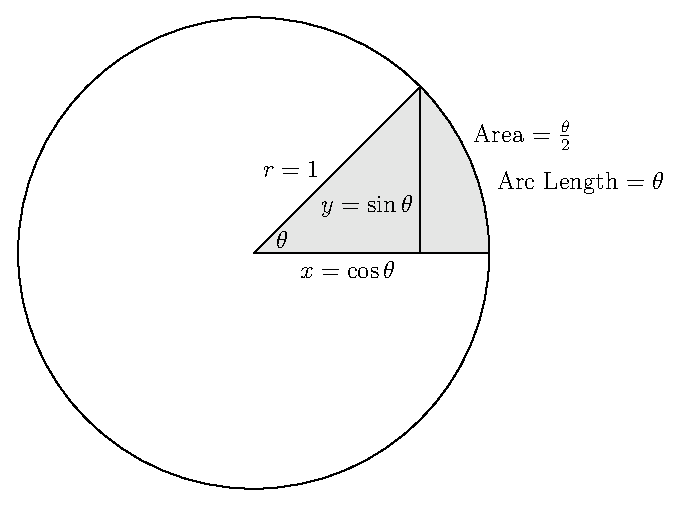
\includegraphics[width=8cm]{figure01.eps}
\caption{Definition of the Trigonometric Functions}
\label{figure-trig-definition}
\end{figure}

The basic idea for hyperbolic functions comes from the
construction of trigonometric functions. Recall how we
defined the sine and cosine functions, as shown in 
Figure \ref{figure-trig-definition}. For a
circle with radius one, angle (in radians) can be \emph{defined}
to be the arc length of the inscribed arc or, equivalently,
twice the shadded area. Then the $x$ and $y$ coordinates of a
point on the edge of the unit circle, dependant on the angle,
are given by the cosine and sine functions, respectively. The
important observation is that there is an \emph{natural,
intrinsic} definition of angle, and that the trigonometric
functions give cartesian ccoordinates based on that intrinsic
angle.

\begin{figure}[hb]
\centering
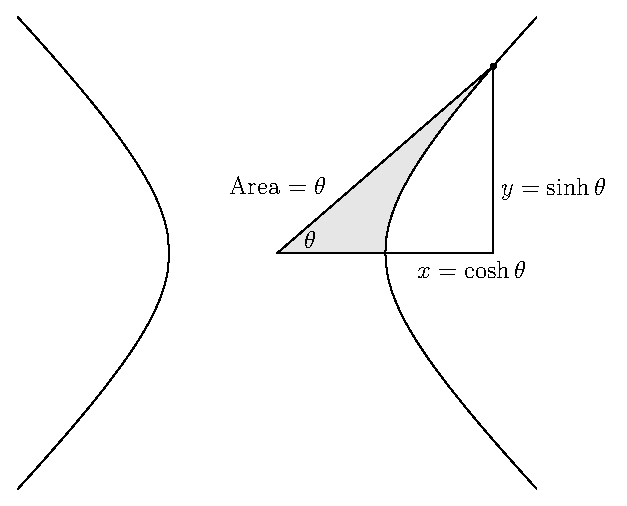
\includegraphics[width=8cm]{figure02.eps}
\caption{Definition of the Hyperbolic Functions}
\label{figure-hyperbolic-definition}
\end{figure}

The unit circle is the locus of the equation $x^2 + y^2 = 1$.
If we change this very slightly to $x^2 - y^2 = 1$, then we
have the unit hyperbola instead. 

\begin{defn}
As seen in Figure \ref{figure-hyperbolic-definition},
\emph{hyperbolic angle} is defined to be the area inscribed by
the hyperbolic. Hyperbolic cosine and sine are the $x$ and $y$
coordinates of a point on the hyperbola as functions of
hyperbolic angle.
\end{defn}

Recall that trigonometric angle is bounded between
0 and $2\pi$. Hyperbolic angle is unbounded: as we keep moving
the point up the hyperbola, the inscribed area grows to
infinity. This also means that hyperbolic function are
\emph{not} periodic.

\subsection{Hyperbolic Identities}
\label{hyperbolic-identities}

The fundamental trigonometric idetity is $\sin^2 \theta +
\cos^2 \theta =1$, which comes from the fact that these are
$x$ and $y$ coordinates and the circle is the locus $x^2 +
y^2 = 1$. For the hyperbolics, the locus is now $x^2 - y^2 =
1$, so the fundamental hyperbolic identity is
\begin{equation*}
\cosh^2 \theta - \sinh^2 \theta = 1.
\end{equation*}
In parallel with the trigonometric functions, there are many
other hyperbolic identities. In almost all cases, they are
the same as the trigonometric identities excepts for
differences in sign. I'll give two examples here; the
rest are found in the reference materials.
\begin{equation*}
\sinh (x+y) = \sinh x \cosh y + \cosh x \sinh y \hspace{2cm}
\tanh^2 x = 1 - \sech^2 x
\end{equation*}
Also in parallel with trigonometry, the remaining hyperbolic
functions, tanh, coth, sech, csch are defined in terms of
hyperbolic sine and cosine. For example, since $\tan x =
\frac{\sin x}{\cos x}$, we also have that $\tanh x =
\frac{\sinh x}{\cosh x}$. 

Now we can move on to the most surprising fact about
hyperbolics, a fact that doesn't (at least at this point) have
any parallel with trigonometry. The fact is this: hyperbolics
are actually not new functions at all. They can be quite
easily built out of exponentials. For the base functions
$\sinh x$ and $\cosh x$, we have
\begin{equation*}
\cosh x = \frac{e^x + e^{-x}}{2} \hspace{1cm} \text{and}
\hspace{1cm} \sinh x = \frac{e^x - e^{-x}}{2}.
\end{equation*}
With this definition, the remaining four hyperbolics are
defined in terms of exponentials as are follows.
\begin{align*}
\tanh x = \frac{e^x - e^{-x}}{e^x + e^{-x}} & \hspace{2cm} 
\coth x = \frac{e^x + e^{-x}}{e^x - e^{-x}} \\
\sech x = \frac{2}{e^x + e^{-x}} & \hspace{2cm} 
\csch x = \frac{2}{e^x - e^{-x}} \\
\end{align*}
In particular, we know the asymptotic behaviour and
asymptotic order of the hyperbolics. $\cosh x$ and $\sinh x$
both have the same asymptotic order as $e^x$. $\sech x$ and
$\csch x$ both have exponential decay to 0. $\coth x$ and
$\tanh x$ both have horizontal asymptotes at $y=\pm1$.

We can also reverse the exponential identities to gives this
pleasant description of the exponential function,
\begin{equation*}
e^x = \cosh x + \sinh x.
\end{equation*}
This leads us to an interesting question. If hyperbolics
relate both to trigonometry (in definition, form and
identities) and exponentials, is there also a hidden
connection between trigonometry and exponentials? This is a
question we will return to late in the course.

\subsection{Inverse Hyperbolics}
\label{inverse-hyperbolics}

For trigonometry, we used the notation of $\arcsin x$ for the
inverse of $\sin x$; we will use a similar notation for
hyperbolics. Inverses will be indicated by a `arc' prefix, so
$\arcsinh x$ is the inverse of the hyperbolic sine function.

The following table summarizes the domain restrictions
required to define the inverse hyperbolics. Since the
hyperbolics are not periodic, these domain restrictions are
much less restrictive than they were for trigonometric
functions. Since the inverse switches domain and range, the
resulting range in the table will be the domain of the
inverse.
\begin{displaymath}
\begin{array}{llll}
\text{Function} & \text{Restricted Domain} & \text{Resulting
Range} & \text{Inverse Function} \\
\hline
\sinh x & \RR & \RR & \arcsinh x \\
\cosh x & [0, \infty) & [0, \infty) & \arccosh x \\
\tanh x & \RR & (-1,1) & \arctanh x \\
\sech x & [0, \infty) & (0, 1] & \arcsech x \\
\csch x & x \neq 0 & x \neq 0 & \arccsch x \\
\coth x & x \neq 0 & (-\infty,-1) \cup (1, \infty) & \arccoth x 
\end{array}
\end{displaymath}
Since the hyperbolics have exponential descripions, we expect
that their inverses will have logarithmic description.
This is true.
\begin{align*}
\arcsinh x & = \ln (x + \sqrt{x^2 +1} ) \\
\arccosh x & = \ln (x + \sqrt{x^2 -1} ) \\
\arctanh x & = \frac{1}{2} \ln \left( \frac{1+x}{1-x} \right) 
\end{align*}

\subsection{Calculus of Hyperbolics}
\label{calculus-hyperbolics}

Now that we have these new functions, we'd like to know their
integral and differential behaviour. The following derivatives
and integrals of hyperbolic functions are all fairly easily
determined using the exponential description. 
\begin{align*}
\frac{d}{dx} \cosh x & = \frac{d}{dx} \frac{e^x + e^{-x}}{2} =
\frac{e^x - e^{-x}}{2} = \sinh x \\
\frac{d}{dx} \sinh x & = \frac{d}{dx} \frac{e^x - e^{-x}}{2} =
\frac{e^x + e^{-x}}{2} = \cosh x \\
\end{align*}
For the remaining four functions, the derivatives are:
\begin{align*}
\frac{d}{dx} \tanh x & = \frac{d}{dx} \frac{\sinh x}{\cosh x} =
\sech^2 x \\
\frac{d}{dx} \coth x & = \frac{d}{dx} \frac{\cosh x}{\sinh x} =
-\csch^2 x \\
\frac{d}{dx} \sech x & = \frac{d}{dx} \frac{1}{\cosh x} =
- \csch x \ \coth x \\
\frac{d}{dx} \csch x & = \frac{d}{dx} \frac{1}{\sinh x} =
- \sech x \tanh x 
\end{align*}
Again, there is a similarity in form to the trigonometric
derivatives but with difference in sign. In particular, for
sine and cosine, four derivatives returned us to the original
function. For hyperbolic sine and cosine, since the
derivatives don't introduce a negative sign, only two
derivatives return us to the original.

One way of thinking about exponentials, trigonometric
functions and hyperbolics is in terms of solutions to
differential equations. This table summarizies three of the
most basic and most important DEs and their solutions (where
$a$ and $b$ are real constants).
\begin{displaymath}
\begin{array}{ll}
\text{DE} & \text{Solution} \\
\hline 
\dfrac{df}{dx} = f & f = ae^x \vspace{.2cm} \\
\dfrac{d^2f}{dx^2} = -f & f = a \sin x + b \cos x
\vspace{.2cm} \\
\dfrac{d^2f}{dx^2} = f & f = a \sinh x + b \cosh x
\end{array}
\end{displaymath}
The derivatives of (most of) the inverse hyperbolic are as follows. 
\begin{align*}
\frac{d}{dx} \arcsinh x & = \frac{1}{x + \sqrt{x^2+1}} \left( 1
+ \frac{2x}{2 \sqrt{x^2+1}} \right) = \frac{\sqrt{x^2+1} + x}{(x
+ \sqrt{x^2+1}) \sqrt{x^2+1}} = \frac{1}{\sqrt{x^2+1}} \\
\frac{d}{dx} \arccosh x & = \frac{1}{\sqrt{x^2-1}} \\
\frac{d}{dx} \arctanh x & = \frac{1}{1-x^2} \\
\frac{d}{dx} \arccoth x & = \frac{1}{1-x^2}
\end{align*}
Like inverse trigonometric derivatives, the results of these
derivatives are particularly interesting because they are
special algebraic functions which don't have algebraic
anti-derivatives. If we reverse the direction, this means we
need inverse hyperbolics to do the following integrals.
\begin{align*}
\int \frac{1}{\sqrt{1+x^2}} dx & = \arcsinh x + c \\
\int \frac{1}{\sqrt{1-x^2}} dx & = \arccosh x + c \\
\int \frac{1}{1 - x^2} dx & = \arctanh x + c \text{ or }
\arccoth x + c
\end{align*}
Notice the strangness with inverse hyperbolic cotangent and
tangent. Both have the same derivatives and both solve the
same integrals. This seems odd, since the
solutions to integrals are unique up to a constant. The
confusion is solved by realizing that $\arccoth$ and $\arctanh$
have mutually exclusive domains. Therefore, the `or' in the
solution is appropriate: the anti-derivative is either of the
two functions depending on your location on the real number
line.

\section{Implicit Derivatives and Plane Curves}
\label{plane-curves}

\subsection{Implicit Derivatives}
\label{implicit-derivatives}

In Calculus I, we mostly calculated slopes of tangent lines to
graphs of functions. These are loci of the form $y = f(x)$,
and $f^\prime(x)$ gave us the slope of the tangent line.
For arbitrary loci in $\RR^2$, such as the conics, tangent
lines can also be defined. We need a refinement of our
derivative techniques to find their slopes, since most loci
are not graphs of functions. The new technique is implicit
differentiation.

Since we know how to differentiate functions, we will
\emph{pretend} that our loci are (at least locally) graphs of
functions. In a locus of $x$ and $y$, we will pretend that $y$
is a function of $x$. We will the use this pretense to
differentiate the expression of the locus.

\begin{figure}[ht]
\centering
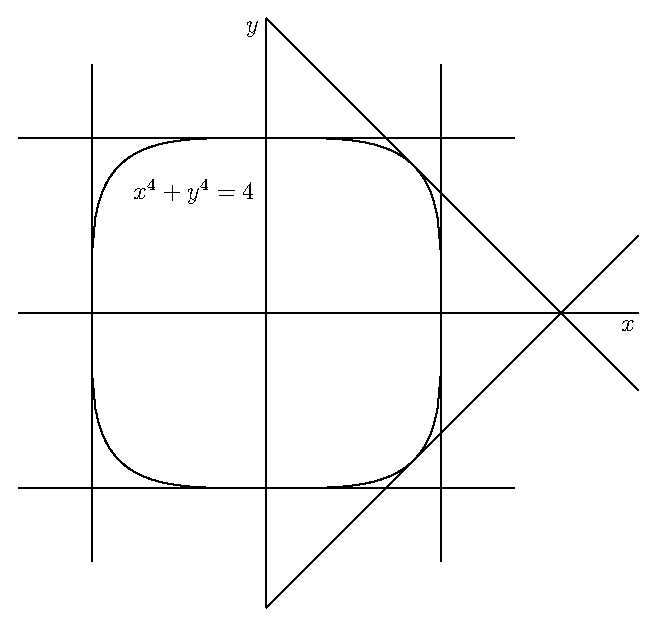
\includegraphics[width=08cm]{figure03.eps}
\caption{Tangent Lines to $x^4 + y^4 =1$}
\label{figure-implicit-example}
\end{figure}

\begin{example}
Take the locus of $x^4 + y^4 = 1$, as in
Figure \ref{figure-implicit-example}
We will pretend that $y$ is locally a function of $x$.
Any expressions in $x$ we differentiate normally. For
expressions in $y$, we use the \emph{chain rule}, due to
the pretense that $y$ is a
function of $x$. Therefore, $y^4$ has a
derivative of the outside ($4y^3$) and a derivative of the
inside ($\frac{dy}{dx}$). Then we solve for $\frac{dy}{dx}$.
\begin{align*}
x^4 + y^4 & = 4 \\
\frac{d}{dx} x^4 + y^4 & = \frac{d}{dx}4 \\
4x^3 + 4y^3 \frac{dy}{dx} & = 0 \\
\frac{dy}{dx} & = \frac{-x^3}{y^3} 
\end{align*}
For any point $(x,y)$ on this locus, the slope of the tangent
at that point is given by the expression $\frac{-x^3}{y^3}$.
The slope is $0$ at the point $(0, \pm \sqrt{2})$. The slope
is undefined at $(\pm \sqrt{2}, 0)$. Other points on the curve
include $(\pm \sqrt[4]{2}, \pm \sqrt[4]{2})$. Here, depending
on the signs, the slope is $1$ or $-1$. Some of these tangent
lines are drawn in Figure \ref{figure-implicit-example}.
\end{example}

Notice that the slope isn't defined everywhere. The slope
approaches vertical near the undefined point $(\pm
\sqrt[4]{2}, 0)$; this makes sense, since a vertical line has
no slope. This is also the point where our assumption, that
$y$ can be expressed as a function of $x$, breaks down.
Implicit derivatives can also fail to find slopes at places
where a loci self-intersects or has a sharp corner. We will
see examples of these in the next section.

\section{Algebraic Plane Curves}
\label{algebraic-plane-curves}

\begin{defn}
Another name for loci in $\RR^2$ is \emph{plane curves}.
An \emph{algebraic plane curve} is a locus where the
expressions are polynomials.
\end{defn}

Algebraic plane curves include all conics as well as the
previous example $x^4 + y^4 = 1$. They are the historical root
of a large branch of mathematics called algebraic geometry,
which deals with the geometry of such polynomial plane curves
and their higher-dimensional analogues. 

\begin{defn}
The \emph{degree} of an algebraic plane curve is the highest
polynomial degree involved in the equation of the curve.
\end{defn}

When we study the geometry of algebraic plane curves, we often 
wonder what happens at problematic points.

\begin{defn}
A point where the tangent line to an algebraic plane curve is
not defined is called a \emph{singularity}. 
\end{defn}

We'll use this section to try to understand the singularities
of simple algebraic plane curves. First, let's talk about the
case of vertical tangent lines. The slope of a vertical line
isn't defined, but the tangent line can exist. Our
singularities are located where a \emph{tangent line} doesn't
exist. Therefore, vertical tangents are fine -- they aren't
singularities. That said, in what follows, we will also get a
method for identifying vertical tangents.

There are, broadly speaking, two types of singularity for
algebraic plane curves: nodes and cusps. 

\begin{defn} 
A \emph{node} occurs at the self-intersection of a plane
curve. We count the number of times the curve overlaps: two
overlaps is often called a \emph{double point}, three a
\emph{triple point}, and so on. A \emph{cusp}, on the other
hand, is a sharp corner. Diagram \ref{figure-singularities} shows
visual examples for algebraic plane curves.
\end{defn}

\begin{figure}[ht]
\centering
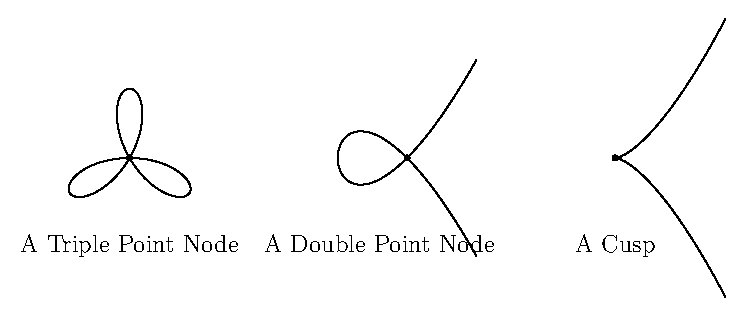
\includegraphics[width=10cm]{figure04.eps}
\caption{Three Plane Curve Singularities}
\label{figure-singularities}
\end{figure}

To understand singularities, we will look at the problematic
points of the implicit derivative. 

\begin{example}Consider the plane curve given by the equation
$y^2 = 4 - 3x^2 - x^3$. This is a degree 3 curve, which
factors as $y^2 = (1-x)(2+x)^2$. (A factored form is often
conveninet for these calculations, when it is possible to find
such a form.) Let's look at the implicit derivative.
\begin{equation*}
2 y \frac{dy}{dx} = -6x - 3x^2 \implies \frac{dy}{dx} =
\frac{-6x-3x^2}{2y}
\end{equation*}
This is well defined except when $y=0$ which, for this curve,
happens at $(1,0)$ and $(-2,0)$.

Let's look at a different form of the implicit derivative,
where we replace $y$ with its expression in $x$.
\begin{equation*}
\frac{dy}{dx} = \frac{-3x(2+x)}{\pm\sqrt{(1-x)(2+x)^2}} =
\frac{-3(2+x)}{\pm\sqrt{1-x} (2+x)}
\end{equation*}
Then we can look at the limits as we approach the undefined
points. When $x=1$, only the denominator goes to $0$, the
numerator is finite. Therefore, we expect the slope diverges to
infinity. This means the tangent line is approaching 
vertical and, in the limit, we recognize a vertical tangent.
There is no singularity here, just a vertical tangent.

This will be our first rule: when the limit of the implicit
derivative approaching an undefined point is $\pm \infty$, we
get a vertical tangent.

However, at $x=-2$, both numerator and denominator have a
$x+2$ term, which can cancel out. (The limit is an
indeterminate form of type $\frac{0}{0}$). Evaluating the
limit gives a slope of $\frac{-3}{\pm\sqrt{3}}$. We get two
slopes, neither of which are vertical. This situation indicates a
self-intersection, with the incoming lines at the two given
slopes. Moreover, since we have two possible tangents, there
are two intersecting pieces and the node is a double point.

This is our second rule: when the limit of the implicit
derivative approaching an undefined point is an indeterminant
form of type $\frac{0}{0}$ which evaluates to several possible
values, we have a node. The number of possible values gives
the number of self-intersections and hence the type of the
node (double point, triple point, etc). Figure
\ref{figure-elliptic-curve1} shows a vertical tangent and a double
point node.
\end{example}

\begin{figure}[ht]
\centering
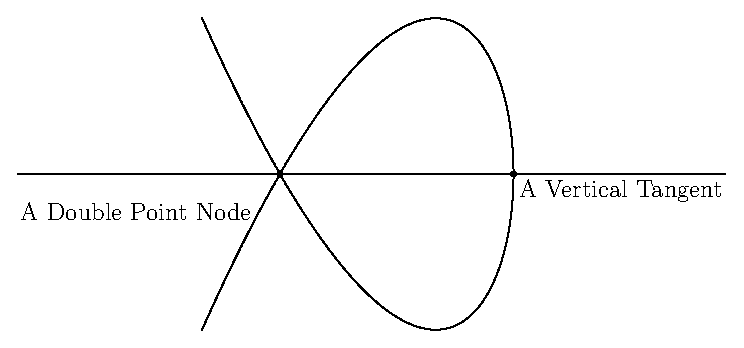
\includegraphics[width=10cm]{figure05.eps}
\caption{The Curve $y^2 = (1-x)(2+x)^2$}
\label{figure-elliptic-curve1}
\end{figure}

\begin{example}
Lastly, consider the curve $y^2 = x^3$ with implicit
derivative $\frac{dy}{dx} = \frac{3x^2}{2y} = \frac{3x^2}{\pm
\sqrt{x^3}}$. This is undefined at the point $(0,0)$ on the
curve, and the limit as we approach the undefined point is
$0$. This behaviour indicates a cusp, which is our third and
final rule: the when the limit of the implicit derivative
approaching an underinfed point is an indeterminant form of
type $\frac{0}{0}$ which evaluates to $0$, then we have a
cusp. Figure \ref{figure-elliptic-curve2} shows a cusp.
\end{example}

\begin{figure}[ht]
\centering
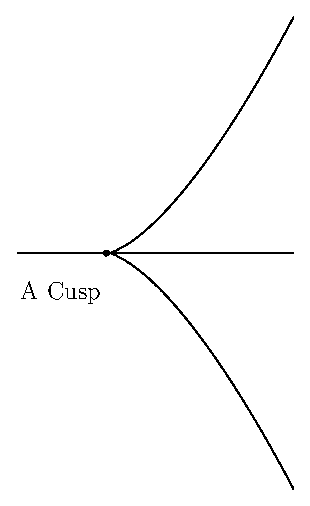
\includegraphics[width=4cm]{figure06.eps}
\caption{The Curve $y^2 = x^3$}
\label{figure-elliptic-curve2}
\end{figure}

\section{Related Rates}
\label{related-rates}

\subsection{Definitions and Reaction Rates}
\label{related-rates-definition}

In applied mathematics, we often have a number of different
quantities that all depend on a common independent variable.
The model can be expressed as the relationship between the various
quantities. In addition, all these quantities typically have
derivatives with respect to the common variable. 

\begin{defn}
A related rates is a relationship between the derivatives of
two or more function (with respect to a common independent
variable).
\end{defn}

\begin{example}
An easy first example is reaction rates in Chemistry. Let's
take a very simple reaction: the product of $NaCl$ salt from
free $Na^+$ and $Cl^-$ ions. We write this reaction as:
\begin{equation*}
Na^+ + Cl^- \rightarrow NaCl
\end{equation*}

Let $N$, $C$ and $S$ (for salt) represent the molar quantity
of the ions or salts and assume that all three are functions
of time. The total amount of material, either sodium or
chlorine, is preserved in time. Mathematically, this is $N + S
= c_1$ or $C + S = c_2$ for some constants $c_1$ and $c_2$.
We can differentiate both equations.
\begin{equation*}
\frac{dN}{dt} = - \frac{dS}{dt} \hspace{1cm} \text{and}
\hspace{1cm} 
\frac{dC}{dt} = - \frac{dS}{dt}
\end{equation*}
The result is what we call a related rate. We have an
original equation between some quantities which all depend on
a common independent variable (here time). We differentiate
in that variable, to get an equation between the various
derivatives. That new equation is a relation between the
rates of change. In this case, the related rate equation
states the very obvious observation that the decrease in $Na^+$ or
$Cl^-$ ions happens as the same rate as the production of
$NaCl$. We really didn't need the heavy machinery of
derivatives to understand this; we could have seen it from the
reaction setup. But this serves as a simple example to
explain the idea of related rates.
\end{example}

To summarize, this is the general procedure for related reates:
\begin{smallparts}
\item Write the relationship between two or more quantities.
(If necessary, use geometry or other information to reduce to
two quantities if more are initially involved.)
\item Realize that all quantities depend on a common variable,
usually time.
\item Differentiate (implicitly) with respect to the common
variable.
\item Solve for the desired rate and see the relationship. 
\end{smallparts}

\subsection{Classic Examples}
\label{classic-examples}

\begin{figure}[ht]
\centering
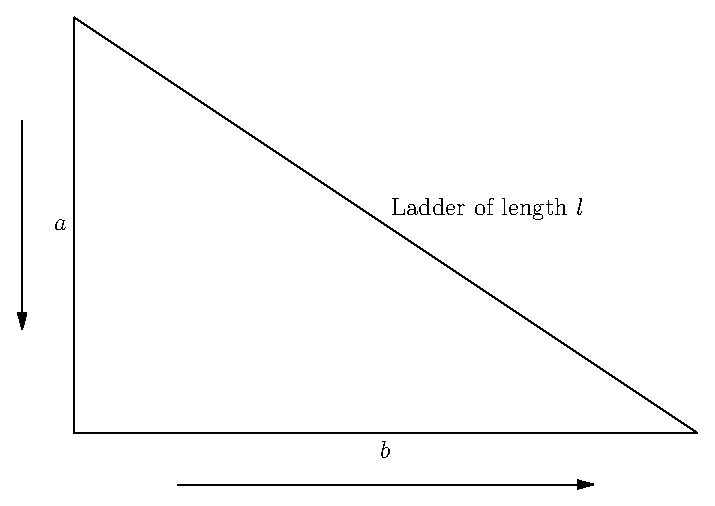
\includegraphics[width=10cm]{figure07.eps}
\caption{The Falling Ladder Problem}
\label{figure-falling-ladder}
\end{figure}

\begin{example}
A classic example seen in almost all calculus texts is the the
falling ladder problem show in Figure \ref{figure-falling-ladder}. A
ladder of length $l$ leans against a wall, where $a$ is the height
along the wall and $b$ is the length from the base of the wall to the
base of the ladder. The ladder is sliding down the wall such that it
always remains in contact with both the wall and the ground. What is
the relationship between the change in $a$ and the change in $b$?

As with most related rates problems, we often have to do some
interpretation or setup to get the equations. The quantities
we care about are the lengths $a$ and $b$. ($l$, the length
of the ladder, is fixed). The geometry here is a right
triangle, so $l^2 = a^2 + b^2$. Since $l$ is constant, this
is the relationship we need between $a$ and $b$. We
differentiate with respect to time.
\begin{equation*}
0 = 2a \frac{da}{dt} + 2b \frac{db}{dt} \implies \frac{da}{dt} =
-\frac{b}{a} \frac{db}{dt} 
\end{equation*}
Notice that this depends on $a$ and $b$. For different values
of $a$ and $b$, we have different relationships, which is
typical for related rates. The original quantities are part of
the equation as well as their derivatives. To get a specific
answer, we have to input some of these values. For example, if
the length of the ladder is $\sqrt{74}$ meters and $a=7$ with
$b=5$ then when $\frac{db}{dt} = 3 m/s$ we calculate
\begin{equation*}
\implies \frac{da}{dt} =
-\frac{b}{a} \frac{db}{dt} = \frac{-5}{7} 3 = \frac{-15}{7}
m/s.
\end{equation*}
If we fed in different values for $a$, $b$ or $\frac{db}{dt}$
we would have a different relationship. 

Also notice that $a$ and $b$ have to be chosen to match the
original geometry. We can take $a=7$ and $b=5$, or $a =
\sqrt{34}$ and $b = \sqrt{40}$, because both give the corred
ladder length in $a^2 + b^2 = l^2$. However, we can't take $a
= 2$ and $b=3$, since they don't satisfy the original
geometry. 

Finally, notice that one derivative is positive while one the
other is negative. This reflects the geometry of the
situation; as with all of applied mathematics, we should
always relate our answer back to the situation and test its
reasonability.
\end{example}

\begin{example}
Another classic example is the melting snowball. Assume
there is a perfectly spherical snowball with radius $r$,
volume $V$ and surface area $A$. Assume also that this
snowball amazingly melts in such a way that it stays
perfectly spherical. What is the relationship between
$\frac{dV}{dt}$, $\frac{dr}{dt}$ and $\frac{dA}{dt}$ as the
snowball melts? Here are the relevant geometric equatios.
\begin{align*}
V & = \frac{4}{3} \pi r^3 \\
A & = 4 \pi r^2 
\end{align*}
We now assume that all these quantities depend on time and we
differentiate.
\begin{align*}
\frac{dV}{dt} & = 4\pi r^2 \frac{dr}{dt} \\
\frac{dA}{dt} & = 8 \pi r \frac{dt}{dt} 
\end{align*}
If we want, we can also rearrange and substitute to find the
related rate equation for $V$ and $A$.
\begin{align*}
\frac{dr}{dt} & = \frac{1}{8\pi r} \frac{dA}{dt} \\
\frac{dV}{dt} & = \frac{4\pi r^2}{8\pi r} \frac{dA}{dt} =
\frac{r}{2} \frac{dA}{dt} 
\end{align*}
\end{example}

\begin{example}
Other common examples of related rates involve fluids moving
between different sizes and shapes of holding tanks. Let's
consider a conical tank draining into a cubical tank. Assume
the conical tank has an angle of $\pi/4$ between it slant and
the vertical and that it drains out of the vertex at the
bottom of the cone. Let's say the height of the conical
tank is 20 meters and it drains into a cubical tank of side
length 10 meters. The related rates question is: given
depths of fluid in each tank ($h_1$ and $h_2$, respectively),
what the relationship between the lowering rate of $h_1$ in
the cone and the rising rate of $h_2$ in the cube?

We need the relationship between the two heights. The
important observation is that the sum of volume of the the
water cone $V_1$ and the volume in the cube $V_2$ is constant.
That is $V_1 + V_2 = c$. Then we can relate the volumes to
the heights.
\begin{equation*}
V_1 = \frac{1}{3} \pi h_1^3 \hspace{1cm} \text{and}
\hspace{1cm} V_2 = 100 h_2
\end{equation*}
That gives this relationship between the heights.
\begin{equation*}
\frac{1}{3} \pi h_1^3 + 100 h_2 = c 
\end{equation*}
We differentiate this relationship.
\begin{align*}
\frac{1}{3} \pi 3h_1^2 \frac{dh_1}{dt} + 100 \frac{dh_2}{dt} & = 0 \\
\frac{dh_1}{dt} & = \frac{-100}{\pi h_1^2} \frac{dh_2}{dt} \\
\frac{dh_2}{dt} & = \frac{-\pi h_1^2}{100} \frac{dh_1}{dt} 
\end{align*}
If, at a certain point in time, we have $h_1 = 2m$ and
$\frac{dh_1}{dt} = -0.05m/2$ what is $\frac{dh_2}{dt}$? We
just use the derived related rates equation.
\begin{equation*}
\frac{dh_2}{dt} = \frac{-\pi h_1^2}{100} \frac{dh_1}{dt} =
\frac{-\pi 2^2}{100} \frac{5}{100} = \frac{-20\pi}{10000} \doteq
0.0063 m/s
\end{equation*}
\end{example}

\begin{example}
For our last example, we can look at gas laws. The ideal gas
law is $PV = nRT$ where $P$ is pressure, $V$ is volume, $n$ is
some (constant) molar quantity of the gas, $R$ is a constant
and $T$ is temperature, which we also assume is constant.
First, let's solve for $P$ and differentiate with respect to
time $t$.
\begin{equation*}
P = \frac{nRT}{V} \implies \frac{dP}{dt} = \frac{-nRT}{V^2}
\frac{dV}{dt} 
\end{equation*}
Likewise, we can solve for $V$ and differentiate with respect
to time.
\begin{equation*}
V = \frac{nRT}{P} \implies \frac{dV}{dt} = \frac{-nRT}{P^2}
\frac{dP}{dt} \implies \frac{dP}{dt} = \frac{-P^2}{nRT}
\frac{dV}{dt}
\end{equation*}
\end{example}

\chapter{Techniques of Integration}
\label{techniques-integration}

\subsection{Solvable Integrals}
\label{solvable}

In Calculus I, we went through many techniques and rules for
differentiation (chain rule, product rule, quotient rule,
etc), but only one major technique for integration (the
substitution rule). In this course, we try to fill in the
remaining major techniques of integration.

Integration is much more difficult than differentiation. Through
we will develop several techniques, they have somewhat
limited application. There are many integrals that simply
defeat all of our methods. 

\begin{example}
On of the best example is the
very useful Gaussian distribution function: $f(x) = e^{-x^2}$.
We consider its integral.
\begin{equation*}
\int e^{-x^2} dx 
\end{equation*}
This is a very useful integral, as we shall see in our section
on probability. However, for our current purposes, it is
entirely unsolvable. There is no function among the
elementary functions that serves as an anti-derivative. In
that sense, the integral is impossible.

In another sense, though, the integral is fine. The integrand
is continuous, so an anti-derivative does exist. We simply
don't have a name for it yet. It's a new, interesting,
unknown function. This is often the case. There are many
integrals we simply can't do with elementary functions. From
the veiwpoint of elementary functions, these are defeats --
impossible integrals. From a broader viewpoint, these are
sources of new and interesting functions.
\end{example}

That said, this section is focused on those integrals which
can be solved by elementary functions. We have several
techniques which apply to particular integral forms and do
give elementary function solutions.

In our study of integration in this course, we will be
expanding upon the use of the substitution from Calculus I. In
many ways, substitution is the most important integration
rule. It behooves us to review the idea. (The remainder of
this section is copied verbatim from the Calculus I notes).

\section{Substitution Rule Review}
\label{substitution-rule}

Since doing integrals is doing derivatives backwards, we might
try to start reversing all the differentiation rules.
Linearity works exactly the same in reverse.
We inverted the power rule in the previous list of
examples. Inverting the product rule starts to become
strange; we postpone that to integration techniques covered in
Calculus II. Arguably the most important differentiation rule is
the chain rule. We will try to reverse it here.

\begin{defn}
If we have $f(g(x))$, then $\frac{d}{dx} f(g(x)) =
f^\prime(g(x)) g^\prime(x)$. Therefore, we can simply reverse
the identity to get: 
\begin{equation*}
\int f^\prime(g(x)) g^\prime(x) = f(g(x)) + c
\end{equation*}
This is called the substitution rule.
\end{defn}

When we covered the chain rule, I recommended labelling the inside
function with a new variable $u = g(x)$. That becomes even
more important here. It's easiest to explain the process by
example.

\begin{example} 
\begin{equation*}
\int 2x (x^2+1)^4 dx 
\end{equation*}
This integral involves a composition. 
Label the inside function $u = x^2 + 1$. Then we
change the entire integral from the variable $x$
to the varaibles $u$. This is a substitution, hence the rule
is called the substitution rule.
We also need to change the differential term $dx$. This term
is strange and confusing, and we really don't have the room
and energy to go into all the historical subtleties of
differentials. If $u =
u(x)$ is the relationthip between $u$ and $x$, then $du =
u^\prime(x) dx$ is the relationship between $dx$ and $du$.
Here $u = x^2 +1$, so $du = (2x) dx$. Let's
rewrite the original integral.
\begin{equation*}
\int (x^2+1)^4 (2x)dx 
\end{equation*}
We can see that substitution works well here: we can
replace $x^2 +1$ with $u$ and $(2x) dx$ with $du$. 
\begin{equation*}
\int u^4 du 
\end{equation*}
We can find the anti-derivative easily by reversing the power
rule.
\begin{equation*}
\int u^4 du = \frac{u^5}{5} + c
\end{equation*}
Then we undo the substitution, by replacing $u$ with $x^2+4$.
\begin{equation*}
\int 2x (x^2+1)^4 dx = \int u^4 du = \frac{u^5}{5} + c =
\frac{(x^2+4)^5}{5} + c
\end{equation*}
\end{example}

\begin{example}
\begin{align*}
\int xe^{x^2} dx & \quad \quad u=x^2 \quad du = 2xdx \\
\int e^u \frac{du}{2} & = \frac{e^u}{2} + c = \frac{e^{x^2}}{2} +
C \\
\int \frac{x}{x-2} dx & \quad \quad u = x-2 \quad du = dx \\
\int \frac{u+2}{u} du & = \int 1 + \frac{2}{u} du \\
& = u + 2 \ln |u| + c = x - 2 + 2\ln|x-2| + c \\
\int \frac{1}{10x-3} dx & \quad \quad u = 10x-3 \quad du = 10dx
\\
\int \frac{1}{u} \frac{du}{10} & = \frac{\ln |u|}{10} + c =
\frac{ \ln| 10x -3 |}{10}
\end{align*}
\end{example}

When we do substitution with definite integrals, we also need
to change the bounds. If $a$ and $b$ are the bounds in $x$
and $u = u(x)$ is the relationship between $u$ and $x$, then
$u(a)$ and $u(b)$ will be the bounds in $u$. One nice thing
about definite integrals is that we can use these new bounds
to evaluate the integral. We don't have to
substitute back after we finish. 

\begin{example}
\begin{align*}
\int_0^2 \frac{2x}{(x^2+1)^2} dx & \quad \quad u x^2+1 \quad du
= 2xdx \quad u(0) = 1 \quad u(2) = 5 \\
\int_1^5 \frac{du}{u^2} & = \left. -\frac{1}{u} \right|_2^5 =
1 - \frac{1}{5} = \frac{4}{5} \\
\int_{-1}^2 x^2 e^{x^3+1} dx & \quad \quad u = x^3+1 \quad du =
3x^2dx \quad u(-1) = 0 \quad u(2) = 9 \\
\int_0^9 e^u \frac{du}{3} & = \left. \frac{e^u}{3} \right|_0^9 =
\frac{e^9}{3} - \frac{1}{3} = \frac{e^9-1}{3} \\
\int_0^{\pi/4} \frac{\sin x}{\cos^3 x} dx & \quad \quad u = \cos
x \quad du = -\sin x dx \quad u(0) = 1 \quad u(\pi/4) =
\frac{\sqrt{2}}{2} \\
\int_1^{\frac{\sqrt{2}}{2}} \frac{-du}{u^3} & = \left.
\frac{2}{u^2} \right|_1^{\frac{\sqrt{2}}{2}} = 4-2 = 2
\end{align*}
\end{example}

\section{Integration by Parts}
\label{parts}

\subsection{Definition}
\label{parts-definition}

The substitution rule is, in some sense, an inverted
chain rule. We can ask: how many other differentiation rules
can be reasonably inverted? The power rule is very directly
inverted and was one of the first examples of integration.
Our of the remaining rules, the most useful rule to invert is
the product rule. 

\begin{defn}
Recall the product rule for differentiation.
\begin{equation*}
\frac{d}{dx} f(x) g(x) = \frac{df}{dx} g + f \frac{dg}{dx} 
\end{equation*}
Let's integrate both sides of this equation.
\begin{align*}
\int \frac{d}{dx} fg dx & = \int \frac{df}{dx} g dx + \int f
\frac{dg}{dx} dx \\
fg & = \int \frac{df}{dx} g dx + \int f
\frac{dg}{dx} dx \\
\int \frac{df}{dx} g dx & = fg - \int f \frac{dg}{dx} dx
\end{align*}
This last line is a new integration rule called
\emph{integration by parts}.
\end{defn}

Like the substitution rule, integration by parts doesn't
solve the integral by itself; instead, it changes the form of
the integral into something which is (hopefully) more
approachable. Also like substitution rule, it often involves
guessing and experimentation to find the right use of
integration by parts, if such a use even exists for a
particular integral.

In applying the substitution rule, I encouraged careful
labelling. The same is true here: I recommend
labelling the terms and being particularly careful with $\pm$
signs. A simplier statemenet of integration by parts, which
may be more useful for your labelling, is this short form:
\begin{equation*}
\int g df = fg - \int f dg
\end{equation*}

\subsection{Examples}
\label{parts-examples}

\begin{example}
The first step in any integration by parts is chooing 
which piece is $f$ and which is $g$ in the technique.
One choice makes the following integral easier and one makes
it more difficult. The first choice we might take is $df = x$
and $g = e^x$.
\begin{align*}
\int x e^x dx & \\
df & = x \implies f = \frac{x^2}{2} \\
g & = e^x \implies dg = e^x \\
\int x e^x dx & = fg - \int f dg = \frac{x^2}{2} e^x - \int 
\frac{x^2}{2} e^x dx 
\end{align*}
This gives a new integral which isn't any easier than the
previous. This use of integration by parts hasn't helped.
Instead, try $df = e^x$ and $g = x$.
\begin{align*}
\int x e^x dx & \\
df & = e^x \implies f = e^x \\
g & = x \implies dg = 1 \\
\int x e^x dx & = xe^x - \int e^x dx = xe^x - e^x = (x-1)e^x + C
\end{align*}
This choice worked, and we were able to continue on to the
complete solution. As with all integration problems, we can
check our answer by differentiation.
\begin{equation*}
\frac{d}{dx} (x-1)e^x + C = e^x \frac{d}{dx} (x-1) + (x-1)
\frac{d}{dx} e^x = e^x + xe^x - e^x = xe^x
\end{equation*}
\end{example}

\begin{example}
\begin{align*}
\int x \cos dx & \\
df & = \cos x \implies f = \sin x \\
g & = x \implies dg = 1 \\
\int x \cos dx & = x \sin x - \int \sin x dx = (x \sin x +
\cos x) + C
\end{align*}
\end{example}

\begin{example}
This example uses integration by parts twice. Pay
attention to the $\pm$ signs.
\begin{align*}
\int x^3 e^x dx & = x^2 e^x - \int 2x e^x = x^2 e^x - \left( 2xe^x
- \int 2e^x dx \right) \\
& = x^3 e^x - 2xe^x + 2e^x + C
\end{align*}
\end{example}

For definite integrals, the technique is almost the same. The only
trick is that for the middle $fg$ term, we must evaluate the
function on the bounds of integration. 

\begin{example}
\begin{equation*}
\int_1^2 x e^x dx = \left. xe^x \right|_1^2 - \int_1^2 e^x dx =
2e^2 - e - \left. e^x \right|_1^2 = 2e^2 - e - e^2 + e = e^2
\end{equation*}
In this example, we choose $df =x^2$ and $g = \ln x$.
\begin{align*}
\int_1^{e^2} x^2 \ln x dx & = \left. \frac{x^3}{3} \ln x
\right|_1^{e^2} - \int_1^{e^2} \frac{x^3}{3} \frac{1}{x} dx \\
& = \frac{e^6}{3} 2 - \frac{1}{3} 0 - \frac{1}{3} \int_1^{e^2}
x^2 dx = \frac{2e^6}{3} - \left. \frac{x^3}{9} \right|_1^{e^2}
\\
& = \frac{2e^6}{3} - \frac{e^6}{9} + \frac{1}{9} = \frac{5e^6 +
1}{9} 
\end{align*}
\end{example}

\begin{example}
The next integrand
doesn't look anything like a product, but we can choose
$f = \ln x$ and $dg = 1$ which allows $g = x$ and $f =
\frac{1}{x}$. 
\begin{equation*}
\int \ln x dx = x \ln x - \int \frac{x}{x} dx = x \ln x - \int 1
dx = x \ln x - x + C
\end{equation*}
\end{example}

\begin{example}
This examples uses a clever
reduction argument. Let $a,b \in \RR$ with $a,b \neq 0$. We
use integration by parts twice in a row.
\begin{align*}
\int e^{ax} \sin bx dx & \\
df & = e^{ax} \implies f = \frac{e^{ax}}{a} \\
g & = \sin bx \implies dg = b \cos bx \\
\int e^{ax} \sin bx dx & = \frac{e^{ax} \sin bx}{a} - \int
\frac{b}{a} e^{ax} \cos bx dx \\
df & = e^{ax} \implies f = \frac{e^{ax}}{a} \\
g & = \cos bx \implies dg = -b \sin bx \\
& = \frac{e^{ax}\sin bx}{a} - \frac{b}{a} \left( \frac{e^{ax}
\cos bx}{a} - \int \frac{b}{a} e^{ax} (-\sin bx) dx \right) \\
& = \frac{e^{ax}\sin bx}{a} - \frac{be^{ax} \cos bx}{a^2} -
\frac{b^2}{a^2} \int e^{ax} \sin bx dx 
\end{align*}

Now we must be particularly inventive. We haven't
solved the integral, but by doing integration by parts twice,
we have recovered the original integral. Now we can
algebraically isolate that integral to provide a solution.
\begin{align*}
\left( 1 + \frac{b^2}{a^2} \right) \int e^{ax} \sin bx dx & =
\frac{ae^{ax} \sin b x - b e^{ax} \cos bx}{a^2} \\
\int e^{ax} \sin bx dx & = \frac{\frac{ae^{ax} \sin b x - b
e^{ax} \cos bx}{a^2}}{\frac{a^2+b^2}{a^2}} \\
\int e^{ax} \sin bx dx & = \frac{ae^{ax} \sin b x - b
e^{ax} \cos bx}{a^2+b^2}
\end{align*}
\end{example}

\begin{example}
In our last example, we start with a substitution and
then use integration by parts.
\begin{align*}
\int_0^{\frac{\pi^2}{4}} \sin \sqrt{x} dx & \\
u = \sqrt{x} & du = \frac{1}{2\sqrt{x}} dx = \frac{1}{2u} dx \\
2udu = dx & u(0) = 0 \hspace{1cm} u(\frac{\pi^2}{4}) =
\frac{\pi}{2} \\
\int_0^{\frac{\pi^2}{4}} \sin \sqrt{x} dx & =
\int_0^{\frac{\pi}{2}} 2u \sin u du & \\
f & = 2u \implies df = 2 \\
dg & = \sin u \implies g = -\cos x\\
\int_0^{\frac{\pi}{2}} 2u \sin u du & = 2u \left. (-\cos u)
\right|_0^{\frac{\pi}{2}} - \int_0^{\frac{\pi}{2}} 2 (-\cos u)
du \\
& = 2 \frac{\pi}{2} \left( -\cos \frac{\pi}{2} \right) + 2
\int_0^{\frac{\pi}{2}} \cos u du = 2 \left. \sin u
\right|_0^{\frac{\pi}{2}} = 2
\end{align*}
\end{example}

\section{Partial Fractions}
\label{partial-fractions}

\subsection{Integrals of Rational Functions}
\label{rational-functions}

By itself, the technique of partial fractions isn't strictly a
technique of integration. Rather, it's an algebraic technique
for rational functions (fractions involving polynomials). We
we be using it to do integrals of rational functions.

There are a number of important rational functions integrals
which we already know (or we can simply look up on the
tables):
\begin{align*}
\int \frac{1}{x^r} dx & = \frac{-1}{(r-1)}{x^r-1} \hspace{1cm} r
\neq 1 \\
\int \frac{1}{x} dx & = \ln |x| + c \\
\int \frac{1}{x+a} dx & = \ln |x+a| + c \\
\int \frac{1}{1+x^2} dx & = \arctan x + c = -\arccot x + c \\
\int \frac{1}{1-x^2} dx & = \arctanh x + c \text{ or } \arccoth x
+ c
\end{align*}

By substitution and manipulation, we can use the integrals in
the previous list to solve any integrals of this type:
\begin{equation*}
\int \frac{1}{ax+b} dx \hspace{2cm} 
\int \frac{1}{ax^2 + bx + c} dx \hspace{2cm} 
\int \frac{2ax+ b}{ax^2+bc+x} dx 
\end{equation*}

We will be using partial fractions to reduce more complicated
rational functions to functions of these three types.

\subsection{Proper Fractions and Long Division}
\label{long-division}

\begin{defn}
A \emph{proper} rational functions is one where the degree of
the numerator is less than the degree of the denmoninator.
\end{defn}

For general rational functions, we can reduce to a proper
fractions by doing polynomial long division. This long
division works exactly like long division worked for numbers.
The only difference is that where long division for numbers
looked at place values, we look at degrees. An example shows
the technique.

\begin{example}
\polylongdiv{x^4+3x^2+2x+4}{x^2+4}

We see that $x^4+3x^2+2x+4$ divided by $x^2+4$ is $x^2-1$
remainder $2x+8$, so we write
\begin{equation*}
\frac{x^4+3x^2+2x+4}{x^2+4} = x^2 - 1 + \frac{2x+8}{x^2+4}
\end{equation*}
In particular, if we were to integrate, we would have 
\begin{equation*}
\int \frac{x^4+3x^2+2x+4}{x^2+4} dx = \int \left( x^2 - 1 +
\frac{2x+8}{x^2+4} \right) dx = \frac{x^3}{3} - x + \int
\frac{2x+8}{x^2+4} dx 
\end{equation*}
Since we have polynomial long division,we only have to solve
integration problems for proper rational functions. 
\end{example}

\subsection{The Algebraic Technique of Partial Fractions}
\label{partial-fractions-technique}

If we add or subtract polynomial, we use common denominator.

\begin{example}
\begin{equation*}
\frac{1}{x-3} + \frac{1}{x+4} = \frac{(x+4) +
(x-3)}{(x-3)(x+4)} = \frac{2x+1}{x^2+x-12}
\end{equation*}
\end{example}

\begin{example}
The process is similar for more complicatied polynomials:
\begin{align*}
\frac{x^2-2}{x^3-3x} + \frac{1}{x^2-4x+3} & = 
\frac{x^2-2}{x^2(x-3)} + \frac{1}{(x-3)(x-1)} \\
& = \frac{(x-1)(x^2-2}{x^2(x-3)(x-1)} + \frac{x^2}{x^2(x-3)(x-1)}
= \frac{(x-1)(x^2-2) + x^2}{x^2(x-3)(x-1)} \\
& = \frac{x^3-2x+2}{x^2(x-3)(x-1)} = 
= \frac{x^3-2x+2}{x^4 - 4x^3+ 3x^2}
\end{align*}
\end{example}

Partial fractions asks the opposite question: if we are given
a complicated rational function, how can we \emph{undo} common
denominator and express the function as a sum of simplier
fractions. Partial fractions is nothing more (or less) than
common denominator done backwards.

The first step of undoing common denominator is factoring
polynomials. We see that the common demoninator in the
previous example is $x^4 - 4x^3 + 3x^2$, but the seperate
fractions have denominators which are \emph{factors} of the
common denomintor. In order to undo common denominator, we
need to factor the denomintor.

Factoring polynomials is, in general, a very difficult task.
Over $\RR$, there are two types of factors: linear and
quadratic. (It is a nice theorem that all polynomials factor
completely into such factors; we are not going to investigate
that theorem in this course). Linear factors have the form
$(x-\alpha)$. A polynomial has a linear factor $(x-\alpha)$
if and only if $\alpha$ is a root of the polynomial, so
finding linear factors is equivalently difficult to finding
roots. This can be done for low degree polynomials, but for
degree five and above, there is no exact process. Even for low
degrees, finding roots is hardly trivial. An quadratic factor
has the form $(x^2 + \alpha x + \beta)$ and is called
irreducible if it has no real roots (so doesn't factor further
into two linear factors). Though the general problem is quite
difficult, we'll be working with polynomials which factor
reasonably.

Now say that $\frac{p(x)}{q(x)}$ is a proper rational function
and $q(x) = q_1(x) q_2(x) \ldots q_r(x)$ is a factorization
into linear and irreducible quadratic factors. Then we want
to find new numerators $p_i$ to undo the common denominator,
as in the following expression.
\begin{equation*}
\frac{p(x)}{q(x)} = \frac{p_1(x)}{q_1(x)} + \frac{p_2(x)}{q_2(x)} + 
\frac{p_3(x)}{q_3(x)} + \ldots + \frac{p_r(x)}{q_r(x)} 
\end{equation*}

\begin{defn}
If we can find these numerators, this decomposition is called
a \emph{partial fraction decomposision}, of often just
`partial fractions.' 
\end{defn}

Partial fractions is a long and difficult process. It's best
to try to understand it through examples.

\begin{example}
\begin{equation*}
\frac{x+2}{x^2- 5x - 6}
\end{equation*}
The denominator factors as $(x-6)(x+1)$, so we look for a
partial fraction decomposition of the following form.
\begin{equation*}
\frac{x+2}{x^2- 5x - 6} = \frac{a}{x-6} + \frac{b}{x+1}
\end{equation*}
We take the right side to common denominator.
\begin{equation*}
\frac{x+2}{x^2- 5x - 6} = \frac{a}{x-6} + \frac{b}{x+1} =
\frac{a(x+1) + b(x-6)}{(x-6)(x+1)} = \frac{(a+b)x +
(a-6b)}{x^2 - 5x -6}
\end{equation*}
Since both polymomials are the same, the numerators must be
the same. 
\begin{equation*}
x+2 = (a+b)x + (a-6b)
\end{equation*}
Polynomials are equal only if their coefficient are equal, so
this gives us two equations:
\begin{align*}
1 & = a+b \\
2 & = a-6b
\end{align*}
We have to solve these two equations for $a$ and $b$. We do
this by isolating and replacing. The first equation gives $a
= 1-b$, which we substitute in the second equation to get $2 =
(1-b) -6b$ which is $1 = -7b$ or $b = \frac{-1}{7}$. The we
substitute back to get $a = 1-b = 1 - \frac{-1}{7} =
\frac{8}{7}$. These are our numerators.
\begin{equation*}
\frac{x+2}{x^2- 5x - 6} = \frac{\frac{8}{7}}{x-6} +
\frac{\frac{-1}{7}}{x-1}
\end{equation*}
Finally, this helps us integrate by splitting the original
integral up into easier pieces.
\begin{align*}
\int \frac{x+2}{x^2- 5x - 6} dx & = \int
\frac{\frac{8}{7}}{x-6} dx +
\int \frac{\frac{-1}{7}}{x-1} dx \\
& = \frac{8}{7} \int \frac{1}{x-6} dx - \frac{1}{7} \int
\frac{1}{x-1} dx \\
& = \frac{8}{7} \ln |x-6| - \frac{1}{7} \ln |x-1| + C
\end{align*}
\end{example}

\begin{example}
\begin{equation*}
\int \frac{x^2+1}{x^3+4x^2+x+6} dx
\end{equation*}
The denominator has $x=-1$ as a root by inspection. (Our
best methods for roots of cubics, for now, is guessing and
testing.) The denominator factors as $(x+1)(x^2-5x+6) =
(x+1)(x-2)(x-3)$. There are three (non-repeated) linear
factors. Therefore, we look for a partial fractions
decomposition of the following form.
\begin{equation*}
\frac{x^2+1}{x^3+4x^2+x+6} = \frac{a}{x+1} + \frac{b}{x-2} +
\frac{c}{x-3} 
\end{equation*}
The new fractions must be proper, so they only have
constant numerators. Our task is to try to find these
unknowns $a$, $b$ and $c$. This is our general process: we
will write the expected expanded form, write the numerators as
unknowns and use common denominator try to find the unknown
coefficients. Let's proceed with this example.
\begin{align*}
\frac{x^2+1}{x^3+4x^2+x+6} & = \frac{a}{x+1} + \frac{b}{x-2} +
\frac{c}{x-3} \\
& = \frac{a(x-2)(x-3) + b(x+1)(x-3) + c(x+1)(x-2)}
{(x+1)(x-2)(x-3)} \\ 
& = \frac{ax^2 -5ax + 6a + bx^2 - 2bx - 3b + cx^2 - cx - 2x}
{(x+1)(x-2)(x-3)} \\ 
& = \frac{(a+b+c)x^2 + (-5a-2b-c)x + (6a-3b-2c)}
{(x+1)(x-2)(x-3)} \
\end{align*}
Since we have equality and the denominators are the same, the
numerators must also be the same.
\begin{equation*}
x^2 + 1 = x^2 + 0x + 1= (a+b+c)x^2 + (-5a-2b-c)x + (6a-3b-2c)
\end{equation*}
Two polynomials are only equal if all their coefficients are
equal, so we can change this into a system of three equations.
(We will always get a linear system here, which is convenient
for those who know linear algebra).
\begin{align*}
a+b+c & = 1 \\
-5a-2b-c & = 0 \\
6a-3b-2c & = 1 
\end{align*}
This is a system of linear equations. There are many ways to
solve such system, but for now we can isolate and replace.
\begin{align*}
a & = 1-b-c \\
& \text{Substitute for $a$ into the second equation} \\
-5(1-b-c) - 2b - c & = 0 \\
-5+5b+5c - 2b -c & = 0 \\
3b + 4c & = 5 \\
b & = \frac{5-4c}{3} \\
& \text{Substitute for $a$ and $b$ into third
equation} \\
6a - 3b -2c & = 1 \\
6(1-b-c) - 3b - 2c & = 1 \\
6-6b-6c-3b-2c & = 2 \\
-9b - 8c & = 5 \\
9 \frac{5-4c}{3} + 8 c & = 5 \\
45 - 36c + 24 c & = 15 \\
-12 c & = -30 \implies c = \frac{10}{3}\\
& \text{Then substitute back} \\
b & = \frac{5 - 4 \frac{10}{3}}{3} = \frac{15-40}{9} =
\frac{-25}{9} \\
a = 1 - b - c & = 1 + \frac{25}{9} - \frac{10}{3} =
\frac{9+25-30}{9} = \frac{14}{9} 
\end{align*}
The values $a = \frac{14}{9}$, $b = \frac{-25}{9}$ and
$c = \frac{10}{3}$ are the appropriate denominators, we
conclude that 
\begin{equation*}
\frac{x^2+1}{x^3-4x^2+x+6} = \frac{\frac{14}{9}}{x+1} -
\frac{\frac{25}{9}}{x-2} + \frac{\frac{10}{3}}{x-3} 
\end{equation*}
Finally, this helps us with integration, since the integral of
the original rational function is now a sum of three easier
integrals.
\begin{align*}
\int \frac{x^2+1}{x^3-4x^2+x+6} dx & = \int
\frac{\frac{14}{9}}{x+1} dx - \int \frac{\frac{25}{9}}{x-2} dx
+ \int \frac{\frac{10}{3}}{x-3} dx \\
& = \frac{14}{9} \int 
\frac{1}{x+1} dx - \frac{25}{9} \int \frac{1}{x-2} dx +
\frac{10}{3} \int \frac{x-3} dx \\
& = \frac{14 \ln |x+1|}{9} - \frac{25\ln |x-2|}{9} +
\frac{10 \ln |x-3|}{3} + c
\end{align*}
\end{example}

\section{Quadratic Types in Partial Fractions}
\label{quadratic-types}

\subsection{Irreducible Factors}
\label{irreducible-factors}

\begin{example}
Here is an example with an irreducible factor.
\begin{equation*}
\int \frac{x^2-x-1}{x^3-3x^2+5x-3} dx
\end{equation*}
The denominator has $x=1$ as a root and it factors as
$(x-1)(x^2-2x+3)$. The discriminant of the quadratic is $-8$, so
it is irreducible and cannot be factored any further.
Therefore, we are looking for a partial fraction decomposition
of the following form.
\begin{equation*}
\frac{x^2- x - 1}{x^3-3x^2+5x+3} = \frac{a}{x-1} +
\frac{bx+c}{x^2-2x+3} 
\end{equation*}
We take the right side to common denominator.
\begin{align*}
\frac{x^2- x - 1}{x^3-3x^2+5x+3} & = \frac{a}{x-1} +
\frac{bx+c}{x^2-2x+3} \\
& = \frac{a(x^2 - 2x + 3) + (bx+c)(x-1)}{x^3-3x^2+5x-3} \\
& = \frac{ax^2 - 2ax + 3a + bx^2 - bx + cx -c}{x^3-3x^2+5x-3} \\
& = \frac{(a+b)x^2 + (-2a-b+c)x + (3a-c)}{x^3-3x^2+5x-3} 
\end{align*}
That gives a system with $a+b=1$, $-2-b+c=-1$ and $3a-c=-1$.
We can use the first and third equations to write everything
in terms of $a$. That gives $b = 1-a$ and
$c = 3a+1$. We replace both in the second equation.
\begin{align*}
-2a + (1-a) + (3a + 1) & = -1 \\
-2a -1 + a + 3a + 1 & = -1 \\
2a & = -1 \implies a = \frac{-1}{2} \\
b & = 1 - \frac{-1}{2} = \frac{3}{2} \\
c & = 3 \frac{-1}{2} + 1 = \frac{-1}{2} 
\end{align*}
This finishes the partial fraction decomposition.
\begin{equation*}
\frac{x^2-x-1}{x^3-3x^2+5x-3} = \frac{\frac{-1}{2}}{x-1} +
\frac{\frac{3}{2} x - \frac{-1}{2}}{x^2 - 2x +3}
\end{equation*}
Then we can integrate.
\begin{equation*}
\int \frac{x^2-x-1}{x^3-3x^2+5x-3} dx = \frac{-1}{2} \int
\frac{1}{x-1} dx + \int \frac{\frac{3}{2} x - \frac{-1}{2}}{x^2 -
2x +3} dx
\end{equation*}
The first term is easy, but now we have a quadratic term.
We solve the quadratic by isolating a piece of it which allows
for a substitution, and completing the square on the remaining
pieces and using an arctan integral. 
\begin{align*}
& \int \frac{\frac{3}{2} x - \frac{-1}{2}}{x^2 -
2x +3} dx \\
& = \frac{3}{4} \int \frac{2x - \frac{2}{3}}{x^2-2x+3}
dx = \frac{3}{4} \int \frac{2x - 2 + (2 - \frac{2}{3})}
{x^2-2x+3} dx \\
& = \frac{3}{4} \left( \int \frac{2x-2}{x^2-2x+3} dx +
\frac{4}{3} \int \frac{1}{x^2-2x+3} dx \right) \\
& = \frac{3}{4} \ln |x^2-2x+3| + \int \frac{1}{(x-1)^2 +2} dx =
\frac{3}{4} \ln |x^2-2x+3| + \frac{1}{\sqrt{2}} \arctan \left(
\frac{x-1}{\sqrt{2}} \right) 
\end{align*}
The whole integral is now complete.
\begin{equation*}
\int \frac{x^2-x-1}{x^3-3x^2+5x-3} dx = \frac{-1}{2} \ln |x-1| +
\frac{3}{4} \ln |x^2-2x+3| + \frac{1}{\sqrt{2}} \arctan \left(
\frac{x-1}{\sqrt{2}} \right) + c 
\end{equation*}
\end{example}

It's useful to have a reference for the process for these
quadratic integrals. The previous example showed us the general
approach: seperate the integral into two pieces, a
substitution piece and an arctangent piece. Consider the
general case.
\begin{equation*}
\int \frac{x + c}{x^2 + ax + b}
\end{equation*}
The derivative of the denominator is $2x + a$, so we can to
manipulate the numerator to make that expression.
\begin{align*}
\int \frac{x + c}{x^2 + ax + b} & = \frac{1}{2} \int \frac{2x +
2c}{x^2 + ax + b} dx \\
& = \frac{1}{2} \int \frac{(2x + a) + (c-a)}{x^2 + ax + b} dx 
& = \frac{1}{2} \int \frac{2x+a}{x^2 + ax+ b} dx + \frac{c-a}{2}
\int \frac{1}{x^2 + ax + b} dx
\end{align*}
Then we can do both integrals. The substitition integral uses
$u = x^2 + ax + b$.
\begin{equation*}
\int \frac{2x + a}{x^2 + ax + b} dx = \ln |x^2 + ax + b|
\end{equation*}
In the second integral, we need to complete the square. Once
we do, we can use the following general form for arctangent
integrals.
\begin{equation*}
\int \frac{1}{(x-\alpha)^2 + \beta^2} dx = \frac{1}{\beta}
\arctan \left( \frac{x-\alpha}{\beta} \right) + C
\end{equation*}

\subsection{Repeated Linear Factors}
\label{repeated-linear-factors}

So far, none of our examples have had repeated factors.
Repeated factors change the process a bit. By themselves,
linear repeated factors are still reasonable to integrate.
\begin{equation*}
\int \frac{3}{(x-2)^2} dx = \int \frac{3}{u^3} dx =
\frac{-3}{2u^2} + c = \frac{-3}{2 (x-2)^2} + c 
\end{equation*}
(For repeated quadratic factors the situation is trickier.
We need reduction formulas or clever manipulations and
substitutions. For this course, we will ignore repeated
quadratic factors.)

For a repeated linear factor $(x-\alpha)^n$, we will look for partial
fractions with the following denominators.
\begin{equation*}
\frac{a_1}{(x-\alpha)} + 
\frac{a_2}{(x-\alpha)^2} + 
\frac{a_3}{(x-\alpha)^3} + \ldots + 
\frac{a_n}{(x-\alpha)^n} + 
\end{equation*}

\begin{example}
\begin{equation*}
\int \frac{2x-3}{(x-1)(x+2)^2}dx 
\end{equation*}
To account for the repeated root, we look for a partial
fraction decomposition of the following form.
\begin{align*}
\frac{2x-3}{(x-1)(x+2)^2} & = \frac{a}{x-1} + \frac{b}{x+2} +
\frac{c}{(x+2)^2} \\
& = \frac{a(x+2)^2 + b(x+2)(x-1) + c(x-1)}
{(x-1)(x-2)^2} \\
& = \frac{ax^2 + 4ax + 4a + bx^2 + bx - 2b + cx -x }
{(x-1)(x-2)^2} \\
& = \frac{(a+b)x^2 + (4a+b+c)x + (4a-2b-c)}
{(x-1)(x-2)^2} 
\end{align*}
We get a system of equations.
\begin{align*}
a+b & = 0\\
4a + b + c & = 2 \\
4a-2b-c & = -3 
\end{align*}
We solve the system. 
\begin{align*}
a & = -b \\
& \text{Substitute this into the second equation} \\
4a + (-a) + c & = 2 \\
3a + c & = 2 \\
a & = \frac{2-c}{3} \\
& \text{Substitute this into the third equation} \\
4a - 2b - c & = -3 \\
4 \frac{2-c}{3} - 2 \frac{c-2}{3} - c & = -3 \\
8 - 4x - 2c + 4 - 3c & = -9 \\
-9c & = -21 \\
c & = \frac{7}{3} \\
a & = \frac{2 - \frac{7}{3}}{3} = \frac{-1}{9} \\
b & = -a = \frac{1}{9} 
\end{align*}
Then we can complete the integral.
\begin{align*}
\int \frac{2x-3}{(x-1)(x+2)^2}dx & = \frac{-1}{9} \int
\frac{1}{x-1} dx + \frac{1}{9} \int \frac{1}{x+2} dx +
\frac{7}{3} \int \frac{1}{(x+2)^2}dx \\
& = \frac{-1}{9} \ln |x-1| + \frac{1}{9} \ln |x+2| + \frac{7}{3}
\frac{-1}{x+2} + c 
\end{align*}
\end{example}

\begin{example}
If we have higher powers of repeated roots, we have additional
terms in the decomposition. We would start a
difficult degree seven example with the following
decomposition.
\begin{equation*}
\frac{1}{(x+1)(x^2+4)^3} = \frac{a}{x+1} + \frac{bx+c}{x^2+4} +
\frac{dc + e}{(x^2+4)^2} + \frac{fx+g}{(x^2+4)^3}
\end{equation*}
The resulting system would a a system of seven equations and
seven variables, which would be laborious to solve.
(Computers, thankfully, are very good at solving system of
linear equations.)
\end{example}

\section{Trigonometric Integrals}
\label{trig-integrals}

\subsection{Strategies}
\label{trig-integrals-strategies}

The trigonometric integrals we've seen so far have been simple
anti-derivatives or integrals found on standard tables. In
this section, we want to expand our repertoire for
trigonometric integrals. We will mostly be considering
integrands which are products of trigonometric functions, such
as $\sin^2 x \cos^3 x$ or $\tan^4 x \sec^2 x$. 

There are several strategies, depending on the form of the
integrand. We have a lot of flexibility with trigonometric
functions, due to the many identities we can apply. There are
two general strategies. First, it is often helpful to
translate everything into sine and cosine. Second, working in
the opposite direction, it is often helpful to use trig
definition to remove fractions, so that we only have
numerators.

\section{Examples}
\label{trig-integrals-examples}

We first look at integrands which involve sine and cosine.
Here there are also several strategies. The first strategy is
substitution, if it works. The most obvious case is when we
have an expression entirely involving sine which is multiplied
by cosine, or vice-versa. These integrals allow for an easy
substitution. 

\begin{example}
\begin{align*}
\int \frac{(1-\cos^4 x)}{\cos^2 x} \sin x dx & \\
u & = \cos x \\
du & = - \sin x dx \\
\int \frac{(1-\cos^4 x)}{\cos^2 x} \sin x dx & = - \int
\frac{1-u^4}{u^2} = -\int \frac{1}{u^2} du + \int u^2 du =
\frac{1}{u} + \frac{u^3}{3} + C \\
& = \sec x + \frac{\cos^3 x}{3} + c
\end{align*}
\end{example}

If a sine or cosine terms shows up with an odd exponent, such
as $\sin^7 x$ or $\cos^3 x$, we can make use of the standard
identity $\sin^2 + \cos^2 =1$ to remove all but one of the
sine or cosine terms. This can be a way to make more
complicated examples into easy substitutions.

\begin{example}
Here cosine shows up with an odd exponent. We change all
but one power of cosine into sine and then use the obvious
substitution.
\begin{align*}
\int \sin^2 x \cos^5 x dx & = \int \sin^2 x \cos^4 x \cos x dx
\\
& = \sin^2 x (1-\sin^2 x)^2 \cos x dx \\
& = \int u^2 (1-u^2)^2 du = \int u^2 - 2u^4 + u^6 du \\
& = \frac{u^3}{3} - \frac{2u^5}{5} + \frac{u^7}{7} + c \\
& = \frac{\sin^3 x}{3} - \frac{2\sin^5 x}{5} + \frac{\sin^7
x}{7} + c
\end{align*}
\end{example}

If we have an expression in sine and cosine where both have
even powers, the previous trick doesn't help. However, we can
use half-angle identities to reduce the exponents. The next
example shows the use of these half-angle identities and the
resulting (admittedly complicated) algebra to finish the
integral. 

\begin{example}
In this example, note that the half-angle identities are used again
in the fourth line, and that the subsitution $u = \sin t$ is
is also seen in the fourth line.
\begin{align*}
\int_0^\pi \sin^2 t \cos^4 t dt & = \int_0^\pi \left(
\frac{1-\cos2t}{2} \right) \left( \frac{1 + \cos2t}{2} \right)^2
dt \\
& = \frac{1}{8} \int_0^\pi (1-\cos 2t) (1+ 2 \cos 2t + \cos^2
2t) dt \\
& = \frac{1}{8} \left( \int_0^\pi dt + \int_0^\pi \cos 2t dt -
\int_0^\pi \cos^2 t dt - \int_0^\pi \cos^3 2t dt \right) \\
& = \frac{1}{8} \left( \pi + \left. \frac{\sin 2t}{2}
\right|_0^\pi - \int_0^\pi \frac{1 + \cos 4t}{2} dt - \int_0^1
(1-\sin^2 2t) \cos 2t dt \right) \\
& = \frac{1}{8} \left( \pi + 0 - \int_0^\pi \frac{1}{2} dt -
\int_0^\pi \frac{\cos 4t}{2}dt - \frac{1}{2} \int_{x=0}^{x=\pi}
(1-u^2) du \right) \\
& = \frac{1}{8} \left( \pi - \frac{\pi}{2} - \left. \frac{\sin
4t}{8} \right|_0^\pi - \left. \frac{1}{2} \left( u -
\frac{u^3}{3} \right) \right|_{x=0}^{x=\pi} \right) \\
& = \frac{1}{8} \left( \pi - \frac{\pi}{2} - 0 - \frac{1}{2}
\left. \left( \sin 2u - \frac{\sin^3 2u}{3} \right)
\right|_0^\pi \right) \\
& = \frac{1}{8} \frac{\pi}{2} = \frac{\pi}{16}
\end{align*}
\end{example}

Sometime when we try to work without denominators, we can't
express everything in terms of sine and cosine. However,
there are integrals than can be entirely expressed in terms of
tangents and secant (or cotangent and cosecent). Like sine
and cosine above, there are some nice strategies for integrals
involving tangent and secant. We can change squares of
tangents into squares of secant using $1 + \tan^2 x = \sec^2
x$. We also know that $\frac{d}{dx} \tan x = \sec^2 x$, so if
we can isolate a $\sec^2 x$ term in an integrand and express
everything else in terms of tangent, a substitution of $u =
\tan x$ should work nicely. 

\begin{example}
Here is an example of a tangent/secant integrand, which we can
solve two ways. In the first method, we convert everything to
cosine and sine and use the techniques mentioned previously.
We work towards a substitution $u = \cos x$ with $du = -\sin x
dx$ and $u(0) = 1$, $u(\frac{\pi}{3}) = \frac{1}{2}$. 
\begin{align*}
\int_0^{\frac{\pi}{3}} \tan^5 x \sec^4 x dx & = 
\int_0^{\frac{\pi}{3}} \frac{\sin^5 x}{\cos^{9} x} dx \\
& = \int_0^{\frac{\pi}{3}} \frac{(1-\cos^2 x)^2}{\cos^{9} x}
\sin x dx \\
& = -\int_1^{\frac{1}{2}} \frac{(1-u^2)^2}{u^{9}} du =
\int_{\frac{1}{2}}^1 \frac{1 - 2u^2 + u^4}{u^{9}} du \\
& = \int_{\frac{1}{2}}^1 \frac{1}{u^{9}} - \frac{2}{u^7} +
\frac{1}{u^5} du = \left. \left( \frac{-1}{8u^{8}} +
\frac{2}{6u^6} - \frac{1}{4u^4} \right) \right|_{\frac{1}{2}}^1
\\
& = \left( \frac{-1}{8} + \frac{1}{3} - \frac{1}{4} +
\frac{2^{8}}{8} - \frac{2^6}{3} + \frac{2^4}{4} \right) \\
& = \frac{-3+8-6+2^{8}\cdot 3 - 2^6 \cdot 8 + 2^4 \cdot
6}{24} \\
& = \frac{-3+8-6+768-512+96}{24} = \frac{351}{24} =
\frac{117}{8}
\end{align*}
Instead of changing the previous example to sine and cosine,
we can isolate an $\sec^2 x$ and use the substitution $u =
\tan x$ with $du = \sec^2 x dx$ and $u(0) = 0$,
$u\left(\frac{\pi}{3} \right) = \sqrt{3}$. 
\begin{align*}
\int_0^{\frac{\pi}{3}} \tan^5 x \sec^4 x dx & = 
\int_0^{\frac{\pi}{3}} \tan^5 x (1 + \tan^2 x) \sec^2 x dx \\
& = \int_0^{\sqrt{3}} u^5 (1+u^2) du = \int_0^{\sqrt{3}} u^5 +
u^7 du \\
& = \left. \frac{u^6}{6} + \frac{u^8}{8}
\right|_0^{\sqrt{3}} = \frac{3^3}{6} + \frac{3^4}{8} 
= \frac{4\cdot 3^3 + 3\cdot 3^4}{24} = \frac{108 + 243}{24} =
\frac{351}{24} = \frac{117}{8}
\end{align*}
\end{example}

Other forms of trigonometric integrals call for the use of
other identities. Since there are so many types of
trigonometric function and trigonometric identity, often these
integrals require creativity and persistance. Also, because of
all the identities involved, there are often numerous
successful approaches. This should be celebrated, but it does
require caution: often two answers from two different process
can look very dissimilar. Both may be correct
anti-derivatives, but a long and complicated series of
identities would be required to relate them. It's very useful
to remember that correct answers can have very different forms
while still being equal.

\begin{example}
We will finish this section with some other uses of
trigonometric identities to simplify integrand. Here's an
integrand with mismatched frequency terms.
\begin{equation*}
\int \sin 2x \cos 5x dx 
\end{equation*}
As useful identity here is the product-to-sum identity. 
\begin{equation*}
\sin Ax \cos Bx = \frac{1}{2} \left( \sin (A-B)x + \sin (A+B)x
\right) 
\end{equation*}
Then we can relatively easily solve the integral.
\begin{align*}
\int \sin 2x \cos 5x dx & = \frac{1}{2} \int \sin (-3x) + \sin
(7x) dx \\
 & = \frac{-1}{6} \cos 3x + \frac{1}{14} \cos 7x + c
\end{align*}
\end{example}

\begin{example}
Here is another tricky example with an unintuitive approach.
\begin{equation*}
\int \frac{dx}{\cos x - 1} dx 
\end{equation*}
We make clever use of the following identity.
\begin{align*}
\sin^2 \left(\frac{x}{2} \right) & = \frac{1-\cos x}{2} \\
\int \frac{dx}{\cos x - 1} dx & = \int \frac{dx}{ -2\sin^2 \left(
\frac{x}{2} \right) } dx = \frac{-1}{2} \int \csc^2 \left(
\frac{x}{2} \right) dx = \cos \left( \frac{x}{2} \right) + c
\end{align*}
\end{example}

Lastly, there are nice symmetry argument for definite
integrals that can help with certain trigonometric integrands.

\begin{example}
The following three integrals are all zero, for reasons of
symmetry. In the first two, we integrate over a whole period
which includes positive and negative pieces. Over a whole
period, those pieces cancel out. In the last integral, we
integrate an odd function over a symmetric domain, so the
positive and negative pieces again cancel out.
\begin{align*}
\int_0^{2\pi} \cos^3 x dx & = 0 \\
\int_0^{\frac{\pi}{2}} \sin^5 4x dx & = 0 \\
\int_{\frac{-\pi}{4}}^{\frac{\pi}{4}} \tan^3 x \cos^2 x & = 0
\end{align*}
\end{example}

\section{Trigonometric Substitutions}
\label{trig-substitutions}

The last major technique for integration is the technique of
trigonometric substitutions. While these are technically just
a new type of substitution, and we already know how to do
substitution, they are a very counter-intuitive class of
substitutions which deserve their own section.

If $x$ is the indepedant variable and $a$ is a constant,
trigonometric substitutions are used for integrals that
involve terms like $\sqrt{a^2 - x^2}$, $\sqrt{x^2 - a^2}$ and
$\sqrt{x^2 + a^2}$. This might seem like very specific set of
integrands to worry about. However, the ubiquitous presence of
the pythagorean theorem in geometric arguments leads to many
integrands of this form. 

So why trigonometry? The idea is to use the square identities 
$\cos^2 x + \sin^2 x = 1$, $1 + \tan^2 x = \sec^2 x$ and
$\cot^2 x + 1 = \csc^2 x$ to simplify the $\sqrt{a^2 \pm x^2}$ terms. 

The following chart outlines the three cases and the
appropriate trig substitution. In each case, the chart give
the term involved in the integrand, the appropriate
substitution, the trig identity that the substitution relies
on, the calculation that removes the square root term and the
domain of application of the substitution.

\begin{align*}
\text{Integrand} \hspace{1cm} 
& \sqrt{a^2 - x^2} \\
\text{Substitution} \hspace{1cm} 
& x = a \sin \theta \\
\text{Identity} \hspace{1cm} 
& \sin^2 \theta + \cos^2 \theta = 1 \\
\text{Calculation} \hspace{1cm} 
& \sqrt{a^2 - x^2} = \sqrt{a^2(1-\sin^2 \theta)} = a \cos \theta \\
\text{Domain} \hspace{1cm} 
& \frac{-\pi}{2} \leq \theta \leq \frac{\pi}{2} \\
\midrule
\text{Integrand} \hspace{1cm} 
& \sqrt{a^2 + x^2} \\
\text{Substitution} \hspace{1cm} 
& x = a \tan \theta \\
\text{Identity} \hspace{1cm} 
& \tan^2 \theta + 1 = \sec^2 \theta \\
\text{Calculation} \hspace{1cm} 
& \sqrt{a^2 + x^2} = \sqrt{a^2(1+\tan^2 \theta)} = a \sec \theta \\
\text{Domain} \hspace{1cm} 
& \frac{-\pi}{2} \leq \theta \leq \frac{\pi}{2} \\
\midrule
\text{Integrand} \hspace{1cm} 
& \sqrt{x^2 - a^2} \\
\text{Substitution} \hspace{1cm} 
& x = a \sec \theta \\
\text{Identity} \hspace{1cm} 
& \tan^2 \theta + 1 = \sec^2 \theta \\
\text{Calculation} \hspace{1cm} 
& \sqrt{x^2 - a^2} = \sqrt{a^2(\sec^2 \theta - 1)} = a \tan \theta \\
\text{Domain} \hspace{1cm} 
& 0 \leq \theta \leq \frac{\pi}{2} 
\end{align*}

\begin{example}
In the first example, we have to remove a constant from the
square root to recognize the $\sqrt{a^2 - x^2}$ form. 
\begin{align*}
\int \sqrt{1-4x^2} dx & = 2 \int \sqrt{\frac{1}{4} - x^2} dx \\
\text{Substitution:} & \\
& x = \frac{1}{2} \sin \theta \\
& dx = \frac{1}{2} \cos \theta d \theta \\
\text{Calculation:} & \\
& \sqrt{\frac{1}{4} - x^2} = \sqrt{\frac{1}{4} - \frac{\sin^2
\theta}{4}} = \frac{1}{2} \sqrt{1 - \sin^2 \theta} = \frac{1}{2}
\cos \theta \\
\text{New Integral:} & \\
\int \sqrt{1-4x^2} dx & = 2 \int \frac{1}{2} \cos \theta
\frac{1}{2} \cos \theta d \theta \\
& = \frac{1}{2} \int \cos^2 \theta d\theta \\
& = \frac{1}{2} \int \frac{1 + \cos 2 \theta}{2} d\theta \\
& = \frac{1}{4} \int d \theta + \int \frac{1}{4} \cos 2 \theta
d\theta \\
& = \frac{\theta}{4} + \frac{\sin 2\theta}{8} + c \\
\text{Reverse Substitution:} & \\
& = \frac{\theta}{4} + \frac{2 \sin \theta \cos \theta}{8} +
c \\
& = \frac{\arcsin 2x}{4} + \frac{2\cdot 2x \sqrt{1-4x^2}}{8} + c
\\
& = \frac{\arcsin 2x}{4} + \frac{x\sqrt{1-4x^2}}{2} + c 
\end{align*}
\end{example}

\begin{example}
\begin{align*}
\int \frac{\sqrt{x^2-9}}{x^3} dx & \\
\text{Substitution:} & \\
x & = 3 \sec \theta \\
dx & = 3 \sec \theta \tan \theta d \theta \\
\text{Calculation:} & \\
\sqrt{x^2-9} & = 3 \sqrt{\sec^2 \theta - 1} = 3 \tan \theta \\
\cos \theta & = \frac{3}{x} \\
\sin \theta & = \sqrt{1 - \frac{9}{x^2}} \\
\text{New Integral:} & \\
\int \frac{\sqrt{x^2-9}}{x^3} dx & = \int \frac{\sqrt{9 \sec^2 \theta -
9}}{27 \sec^3 \theta} 3 \sec \theta \tan \theta d \theta \\
& = \frac{1}{3} \int \frac{\tan^2
\theta}{\sec^2 \theta} d \theta \\
& = \frac{1}{3} \int \sin^2 \theta d\theta \\
& = \frac{1}{3} \int
\frac{1-\cos 2\theta}{2} d \theta \\
& = \frac{1}{3} \int \frac{1}{2}
d \theta - \frac{1}{3} \int \frac{\cos 2\theta}{2} d\theta \\
& = \frac{\theta}{6} - \frac{\sin 2\theta}{12} + c \\
& = \frac{\theta}{6} - \frac{2 \sin \theta \cos \theta}{12} + c \\
\text{Reverse Substitution:} & \\
& = \frac{\arcsec\left(\frac{x}{3} \right)}{6} - \frac{1}{6}
\sqrt{1 - \frac{9}{x^2}} \frac{3}{x} + c \\
& = \frac{\arcsec\left(\frac{x}{3} \right)}{6} -
\frac{\sqrt{x^2-9}}{2x^2} + c 
\end{align*}
\end{example}

\begin{example}
Here is an example with bounds. This particular example is
quite useful: it calculates the area of the ellipse
$\frac{x^2}{a^2} + \frac{y^2}{b^2} = 1$. It restricts
to the quarter of the ellipse in the first quadrant, where the
area is the area under the curve $y = \frac{b}{a}
\sqrt{a^2-x^2}$ for $x \in [0,a]$. Working with the bounds
is difficult: to get the new bounds in $\theta$, we have to
invert the trig functions. Remember the standard choices for
inverting trig functions, or simply work by intuition. Using
special triangles is often convenient.
\begin{align*}
A & = 4 \int_0^a \frac{b}{a} \sqrt{a^2-x^2} dx \\
\text{Substitution:} & \\
& x = a \sin \theta \\
& dx = a \cos \theta d \theta \\
\text{Bounds:} & \\
& x = 0 \implies \theta = 0 \\
& x = a \implies \theta = \frac{\pi}{2} \\
\text{New Integral:} & \\
A & = 4 \int_0^{\frac{\pi}{2}} \frac{b}{a} \sqrt{a^2 - a^2
\sin^2 \theta} a \cos \theta d \theta \\
& = \frac{4ba^2}{a} \int_0^{\frac{\pi}{2}} \cos^2 \theta
d\theta \\
& = 4ab \int_0^{\frac{\pi}{2}} \frac{1 + \cos 2\theta}{2}
d\theta \\
& = \frac{4ab}{2} \left( \int_0^{\frac{\pi}{2}} 1 d\theta
+ \int_0^{\frac{\pi}{2}} \cos 2\theta d\theta \right) \\
& = \frac{2ab\pi}{2} + \left. 2ab\frac{\sin 2\theta}{2}
\right|_0^{\frac{\pi}{2}} = \pi ab + 0 - 0 = \pi ab
\end{align*}
Therefore, the area of an ellipse with major axis $a$ and minor axis $b$
is $\pi ab$. This notion of area reduces to the area of a
circle, where $a=b$ and we get $\pi a^2$ for $a$ the radius.
\end{example}

\begin{example}
Here is another long example with bounds. 
\begin{align*}
\int_{\frac{\sqrt{2}}{3}}^{\frac{2}{3}}
\frac{dx}{x^5\sqrt{9x^2-1}} &
= \int_{\frac{\sqrt{2}}{3}}^{\frac{2}{3}} \frac{dx}{3x^5\sqrt{x^2 -
\frac{1}{9}}} \\
& u = \frac{1}{3} \sec \theta \\
& du = \frac{1}{3} \sec \theta \tan \theta d \theta \\
& u = \frac{\sqrt{2}}{3} \implies \sec \theta = \sqrt{2}
\implies \cos \theta = \frac{1}{\sqrt{2}} \implies \theta =
\frac{\pi}{4} \\
& u = \frac{2}{3} \implies \sec \theta = 2 \implies \cos \theta
= \frac{1}{2} \implies \theta = \frac{\pi}{3} \\
\int_{\frac{\sqrt{2}}{3}}^{\frac{2}{3}} \frac{dx}{3x^5
\sqrt{x^2 - \frac{1}{9}}} 
& = \int_{\frac{\pi}{4}}^{\frac{\pi}{3}} \frac{\frac{1}{3} \sec
\theta \tan \theta d\theta}{3 \frac{\sec^5 \theta}{3^5}
\sqrt{\frac{\sec^2 \theta}{9} - \frac{1}{9}}} \\
& = \int_{\frac{\pi}{4}}^{\frac{\pi}{3}} \frac{3^6}{3^2}
\frac{\tan \theta}{\sec^4 \theta \tan \theta} d \theta \\
& = 81 \int_{\frac{\pi}{4}}^{\frac{\pi}{3}} \cos 4 \theta d
\theta \\
& = 81 \int_{\frac{\pi}{4}}^{\frac{\pi}{3}} \left( \frac{1 +
\cos 2\theta}{2} \right)^2 d \theta \\
& = 81 \left( \int_{\frac{\pi}{4}}^{\frac{\pi}{3}} \frac{1}{4}
d\theta + \int_{\frac{\pi}{4}}^{\frac{\pi}{3}} \frac{\cos
2\theta}{2} d \theta + \int_{\frac{\pi}{4}}^{\frac{\pi}{3}}
\frac{\cos^2 2 \theta}{4} d\theta \right) \\
& = 81 \left( \frac{\frac{\pi}{3} - \frac{\pi}{4}}{4} + \left.
\frac{\sin 2\theta}{4} \right|_{\frac{\pi}{4}}^{\frac{\pi}{3}}
+ \int_{\frac{\pi}{4}}^{\frac{\pi}{3}} \frac{\cos^2 2\theta}{4}
d \theta \right) \\
& = 81 \left(\frac{\pi}{48} + \frac{\sqrt{3}}{8} - \frac{1}{4} + 
\int_{\frac{\pi}{4}}^{\frac{\pi}{3}} \frac{1}{8} d\theta +
\int_{\frac{\pi}{4}}^{\frac{\pi}{3}} \frac{1 + \cos 4\theta}{8}
d\theta \right)\\
& = 81 \left(\frac{\pi}{48} + \frac{\sqrt{3}}{8} - \frac{1}{4} +
\frac{\pi}{96} + \left. \frac{\sin 4\theta}{32}
\right|_{\frac{\pi}{4}}^{\frac{\pi}{3}} \right) \\
& = 81 \left(\frac{\pi}{48} + \frac{\pi}{96} \frac{\sqrt{3}}{8}
- \frac{1}{4} - \frac{\sqrt{3}}{64} + 0 \right)\\ 
& = 81 \left( \frac{2\pi + \pi}{96} + \frac{8\sqrt{3} -
\sqrt{3}}{64} - \frac{1}{4} \right) = 81 \left( \frac{3\pi}{96}
+ \frac{7\sqrt{3}}{64} - \frac{16}{64} \right) \\
& = 81 \left( \frac{\pi}{32} + \frac{7\sqrt{3} - 16}{64} \right)
= \frac{81}{64} ( 2\pi + 7\sqrt{3} - 16)
\end{align*}
\end{example}

\section{Improper Integrals}
\label{improper-integrals}

\begin{example}
We could try to calculate the following integral.
\begin{equation*}
\int_0^2 \frac{1}{\sqrt{x}} dx = \int_0^2 x^\frac{-1}{2} dx 
= \left. 2x^{\frac{1}{2}} \right|_0^2 = 2\sqrt{2} - 0 =
2\sqrt{2}
\end{equation*}
We get a nice, finite answer. However, this is a
bit surprising. Look at the graph of the function in Figure
\ref{figure-improper-integral1}.
\end{example}

\begin{figure}[ht]
\centering
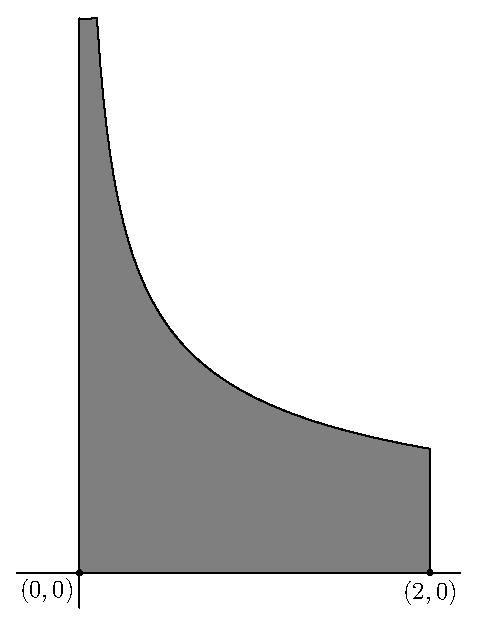
\includegraphics[width=4cm]{figure08.eps}
\caption{An Improper Integral}
\label{figure-improper-integral1}
\end{figure}

The function has a vertical asymptote at $x=0$, which is the
edge of the domain of definition. The function approaches
$\infty$ at the edge of the integral. What does this mean for
the area under the curve? Infninity makes the notion of area
problematic. 

\begin{defn}
An integral which involves an asymptote or other infinite
situation is called an \emph{improper integral}. 
\end{defn}

\begin{example}
Sometimes it's not the function that's infinite, but the
bounds, as in the following integral and the graph in Figure
\ref{figure-improper-integral2}.
\begin{equation*}
\int_1^\infty \frac{1}{x^2} dx
\end{equation*}

\begin{figure}[t]
\centering
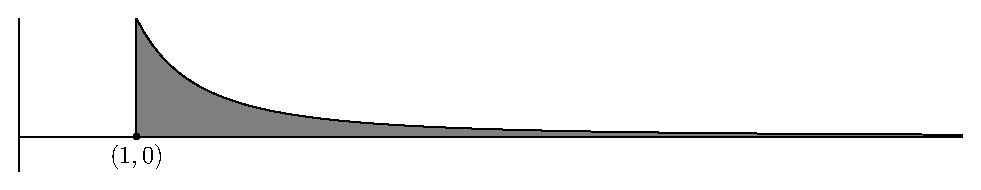
\includegraphics[width=12cm]{figure09.eps}
\caption{Another Improper Integral}
\label{figure-improper-integral2}
\end{figure}

It's not at all obvious how much area there is under the
integral as the bounds go off to infinity. For improper
integrals, we need techniques to deal with these infinities.

The technique, unsurprisingly, involves limits. For the first
integral (even though we could evaluate it conventionally) the
problem exists with the bound $0$, where the function
approaches $\infty$. We define the improper integral using a
limit to approach the asymptote.
\begin{equation*}
\int_0^2 \frac{1}{\sqrt{x}} dx = \lim_{a \rightarrow 0}
\int_a^2 \frac{1}{\sqrt{x}} dx
\end{equation*}
The limit integral is perfectly well defined for $a>0$, since
it avoids the asymptote of the function. 
\begin{equation*}
\lim_{a \rightarrow 0} \int_a^2 x^\frac{-1}{2} = \lim_{a
\rightarrow 0} \left. 2\sqrt{x} \right|_a^2 = \lim_{a
\rightarrow 0} 2 \sqrt{a} - 0 = 2 \sqrt{2}
\end{equation*}
\end{example}

\begin{example}
The same techniques applies to the infinite bounds.
\begin{equation*}
\int_1^\infty \frac{1}{x^2} dx = \lim_{a \rightarrow \infty}
\int_1^a \frac{1}{x^2} dx = \lim_{a \rightarrow \infty}
\left. \frac{-1}{x} \right|_1^a = \lim_{a \rightarrow \infty}
\frac{-1}{a} + 1 = 1
\end{equation*}
In this way, we see that the unknown area under the curve of
$\frac{1}{x^2}$ is indeed finite, even when the bound goes to
infinity. However, infinite area can also happen. 
\end{example}

\begin{example}
Consider a very similar integral.
\begin{equation*}
\int_1^\infty \frac{1}{x} dx = \lim_{a \rightarrow \infty}
\int_1^a \frac{1}{x} dx = \lim_{a \rightarrow \infty}
\left. \ln |x| \right|_1^a = \lim_{a \rightarrow \infty}
\ln a - 0 = \infty 
\end{equation*}
\end{example}

\begin{defn}
With improper integrals, finite answers are not guaranteed.
If the integral is indeed finite, we say that the improper
integral \emph{converges}. Otherwise, we say that the
improper integral \emph{diverges}. 
\end{defn}

\begin{example}
Let's look more carefully at the previous two examples. Both
had integrands of the form $\frac{1}{x^p}$ for some exponent
$p$. We know that $p=1$ gives a divergent integral and $p=2$
gives a convergent integral. If $p < 1$ then $\frac{1}{x^p}
> \frac{1}{x}$. If one positive function is larger than
another, then the area under its graph must be larger.
Since the area under $\frac{1}{x}$ between $1$ and $\infty$ is
already $\infty$, the integral of $\frac{1}{x^p}$ on
$(1,\infty)$ must also be $\infty$. 

Now, if $p<1$, let's make the general calculation.
\begin{align*}
\int_1^\infty \frac{1}{x^p} = \lim_{a \rightarrow \infty}
\int_1^a \frac{1}{x^p} dx = \lim_{a \rightarrow \infty} \left.
\frac{-1}{(p-1)x^{p-1}} \right|_1^a = \lim_{a \rightarrow
\infty} \frac{1}{p-1} -\frac{1}{(p-1)a^{p-1}} = \frac{1}{p-1}
\end{align*}
For, for $p>1$, these all converge. However, $p$ gets close
to $1$, the values of the integrals get very large. $p=1$ is
the crossover point, where the area under the curve becomes
infinite.
\end{example}

We've already implicitly used a comparison argument. We said
that $\frac{1}{x^p} > \frac{1}{x}$ for $p<1$ and used that
fact to argue convergence. This comes from a general property
of integrals: if $f(x) \geq g(x)$ on $[a,b]$, then 
\begin{equation*}
\int_a^b f(x) dx \geq \int_a^b g(x)
\end{equation*}
The same inequality holds for improper integrals, if we allow
the obvious statement that $\infty > a$ for any finite number
$a$. This type of comparison is useful for evaluating
improper integrals. However, a more useful comparison makes
use of asymptotic analysis. I'll state the result this way:
the asymptotic order of a integrand determines the convergence
of an improper integral. 

What does this mean? If means that if we only care about
convergence/divergence (and not the exact value of the
integral), then we only need to consider the asymptotic order
of the integrand. 

\begin{example}
\begin{equation*}
\int_1^\infty \frac{1}{4 + x + 18x^2}
\end{equation*}
The asymptotic order of the denominator is $x^2$. Therefore,
the convenge behaviour is the same as if the integrand were
$\frac{1}{x^2}$. This is $p=2$, which is $p>1$, so the
integral converges. This use of asymptotic order allows us to
dramatically simply the situation: we don't have to evaluate
the complicated quadratic integral to determine convergence or
divergence. (We would, of course, have to evaluate the
complicated quadratic integral if we wanted to determine the
exact value of the improper integral).
\end{example}

\chapter{Applications of Integrations}
\label{integration-applications}

\section{Parametric Curves}
\label{parametric-curves}

We've done a fair bit of work with loci in this course and in
Calculus I. Earlier in this course we talked about algebraic
plane curves, which were the loci of polynomial equations in
$\RR^2$. This section introduces a new way to think about
curves: by thinking of movement along the shape. The movement
happens with respect to a parameter, which we think of as
time: as time passes, we move along the curve. For loci like
algebraic plane curves, the entire curve is presented at one,
as a complete object. For parametric curves, we start at a
point and move along the curve in time.

\subsection{Definition}
\label{parametric-curves-definition}

\begin{defn}
Let $t$ be an indepedent variable (the parameter), which we
think of as time. A parametric curve in $\RR^2$ is a set of
two functions $x(t)$ and $y(t)$, which give the $x$ and $y$
coordinates of the curve at any point $t$ in time. We assume
that $x$ and $y$ are continuous, so that the curve is a
connected curve. Often we want to refer the curve with one
symbol, which is typically the greek letter $\gamma$.
\begin{equation*}
\gamma(t) = (x(t), y(t))
\end{equation*}
Since this is a function of $t$, we need a domain. Typically
we will have $t \in [a,b]$ for an interval.
\end{defn}

\section{Examples}
\label{parametric-curves-examples}

\begin{example}
Consider the curve $\gamma_1(t) = (t,t)$ for $t \in [0,5]$.
This curves gives the line $y=x$, starting at $(0,0)$ and
ending at $(5,5)$. At $t=0$, the curve is at $(0,0)$, at
$t=1$, it is at $(1,1)$, and so on. All parametric curves are
about movement: this is not only the line $y=x$, but also the
starting point $(0,0)$, the ending point $(5,5)$ and the rate
of movement along the line.
\end{example}

\begin{example}
Consider the curve $\gamma_2(t) = (-t,-t)$ for $t \in [-5,0]$.
This is exactly the same line, since it still satisfies $y=x$.
However, now we start at $(5,5)$ when $t=-5$, and we move
towards $(0,0)$ when $t=0$. 
\end{example}

\begin{example}
Now consider the curve $\gamma_3(t) = (t^2,t^2)$ for $t \in
[0,\sqrt{5}]$. Again, this is the same line and, like
$\gamma_1$, it starts at $(0,0)$ and ends at $(5,5)$.
However, it travels the distance a smaller parameter domain,
meaning that it moves faster.
\end{example}

\begin{figure}[ht]
\centering
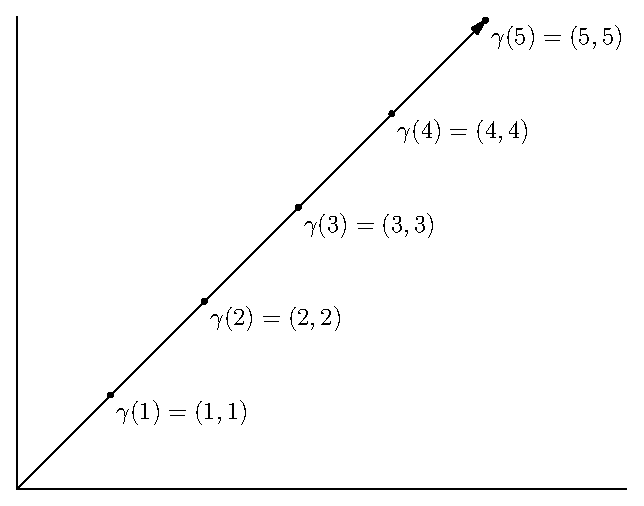
\includegraphics[width=10cm]{figure10.eps}
\caption{Parametric Curve $\gamma_1(t) = (t,t)$}
\label{figure-parametric-curve1}
\end{figure}

\begin{example}
A classic example is $\gamma(t) = (\cos t, \sin t)$ for $t \in
[0,2\pi]$. This curve is just the unit circle, traced counter
clockwise, starting at $(1,0)$. We could change the parameter
domain. If we have $t \in [0,8\pi]$, then we have four
periods of $\sin t$ and $\cos t$, so this traces the same
circle four times. This is a good example of a parametric
curve which traces over itself some number of times.
\end{example}

\begin{example}
Curves can quickly get complicated. Consider this curve:
$\gamma(t) = (\cos 3t, \sin 5t)$. This gives a lovely pattern,
perhaps reminiscent of spirographs (depending on your childhood
experience, of course). The curve is shown in Figure
\ref{figure-parametric-curve2}.
\end{example}

\begin{figure}[ht]
\centering
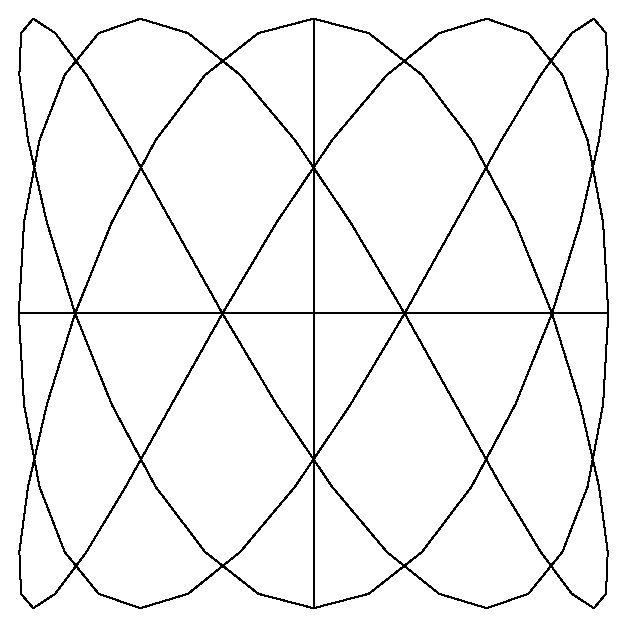
\includegraphics[width=8cm]{figure11.eps}
\caption{$\gamma(t) = (\cos 3t, \sin 5t)$}
\label{figure-parametric-curve2}
\end{figure}

\begin{example}
The next example is called the cycloid. Many curves have
history going back hundreds or thousands of years in geometry,
as evidenced by their greek names. The cycloid is the curve
$\gamma(t) = (a(t-\sin t), a(1-\cos t))$. It describes the
movement of a point at the edge of a wheel as the wheel rolls.
\end{example}

\begin{figure}[ht]
\centering
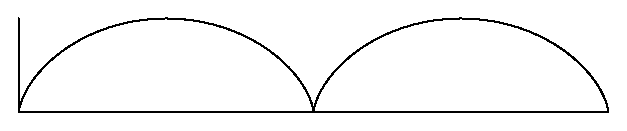
\includegraphics[width=14cm]{figure12.eps}
\caption{The Cycloid}
\label{figure-parametric-curve3}
\end{figure}

Many parametric curves are spirals. The general form for a
spiral is $\gamma(t) = (f(t) \cos t, f(t) \sin t)$ for $f(t)$
a positive monotonic function. $f(t)$ represents the change
in radius as we go around a circle.

\begin{example}
The archemidean spiral is this curve: $\gamma(t) = (t \cos t,
t \sin t)$. It has linear growth in its radius, so there are
equally spaced spiral arms.
\end{example}

\begin{figure}[ht]
\centering
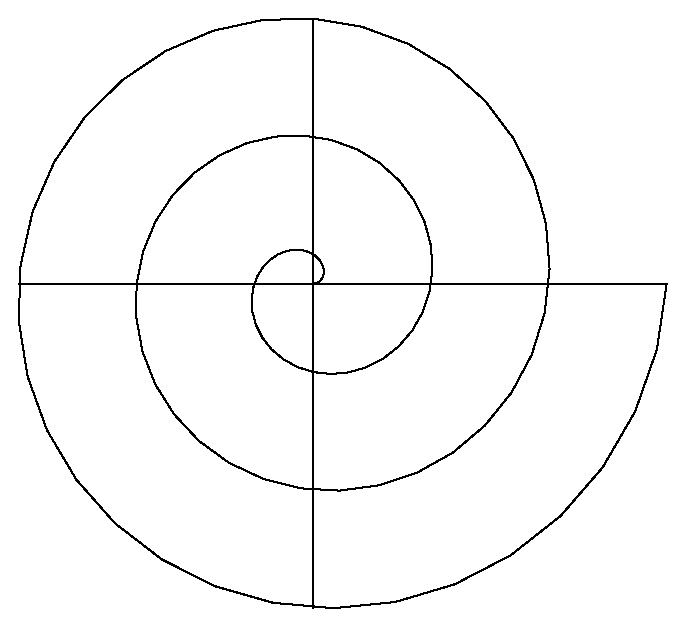
\includegraphics[width=7cm]{figure13.eps}
\caption{The Archimedian Spiral}
\label{figure-parametric-curve4}
\end{figure}

\begin{example}
The hyperbolic spiral is an inward spiral, (it has decreasing
radius). Its expression is $\gamma(t) = (\frac{\cos t}{t},
\frac{\sin t}{t})$. 
\end{example}

\begin{figure}[ht]
\centering
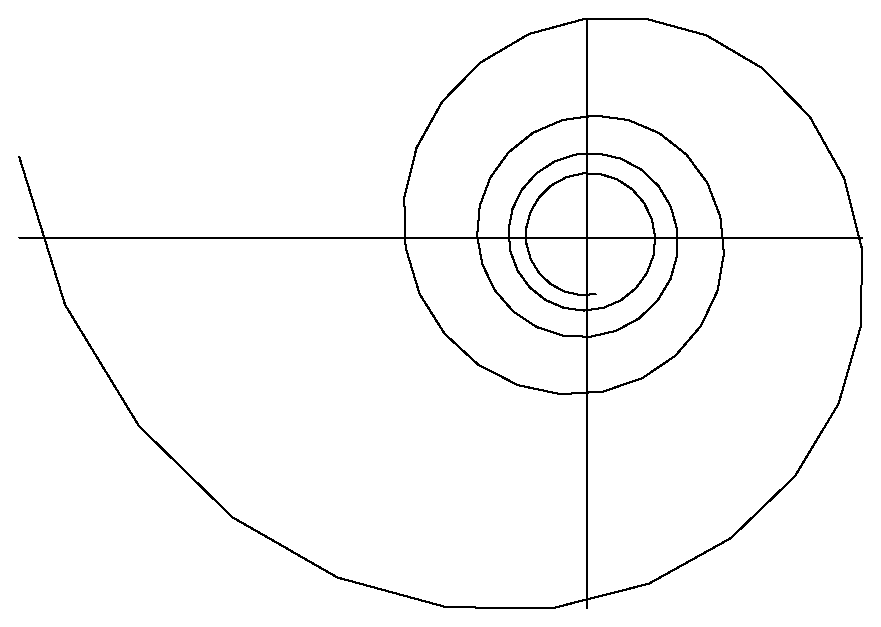
\includegraphics[width=8cm]{figure14.eps}
\caption{The Hyperbolic Spiral}
\label{figure-parametric-curve5}
\end{figure}

\begin{example}
The last spiral in our examples is the logarithmic spiral
which has exponential growth in radius. Its form is
$\gamma(t) = (e^{t} \cos t, e^{t} \sin t)$. 
\end{example}

\begin{figure}[ht]
\centering
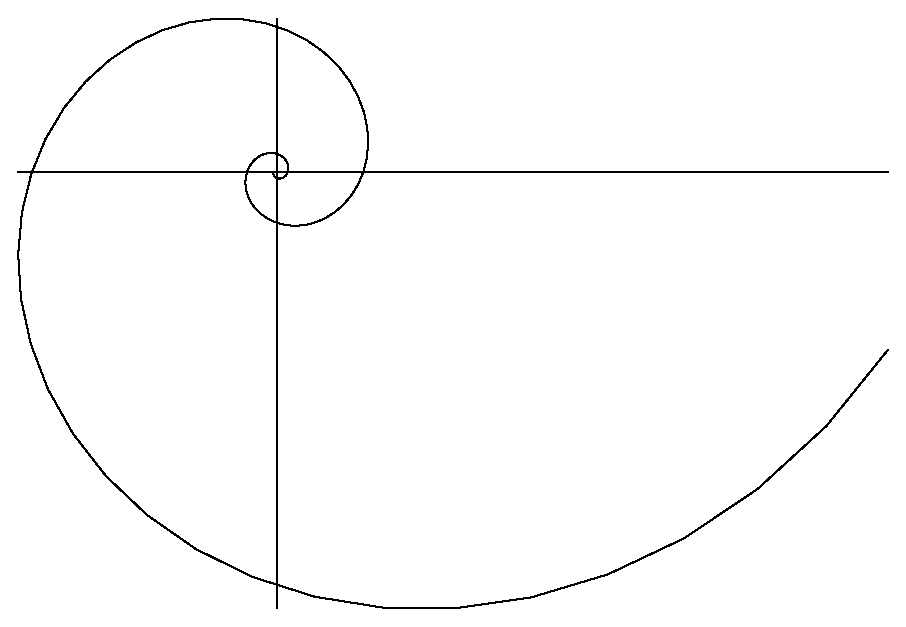
\includegraphics[width=8cm]{figure15.eps}
\caption{The Logarithmic Spiral}
\label{figure-parametric-curve6}
\end{figure}

The logarithmic spiral shows up frequently, both in
mathematics and the natural world. Examples of natural
logarithmic spirals include nautilus shells and spiral
galaxies (though the natural application of the logarithmic
spiral is not without some contraversy).

\begin{example}
A final example, which is not a spiral, is the cardiod. It has
the form $\gamma(t) = ((1-\sin t) \cos t, (1-\sin t) \sin t$.
The name comes from its vaguely heart-shaped path.
\end{example}

\begin{figure}[ht]
\centering
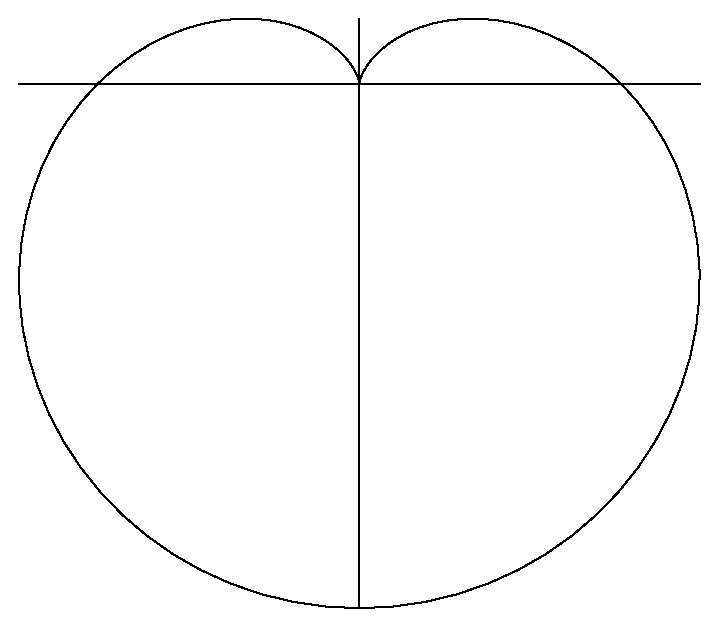
\includegraphics[width=7cm]{figure16.eps}
\caption{The Cardiod}
\label{figure-parametric-curve7}
\end{figure}

\subsection{Reparametrization}
\label{reparametrization}

A parametric curve is more than just a shape in $\RR^2$. The
curve also records the start, end and direction, as well as
the rate of movement along the shape. All that information
depends on the \emph{parametrization}: the way in which
position depends on the parameter.

Sometimes we want to adjust the movement along the shape,
while preserving the shape. We can do that by changing the
parametrization: this is called \emph{reparametrization}. The
idea is to replace the parameter $t$ by a new parameter $s$.
Say we have a curve $\gamma(t) = (x(t),y(t))$, but we can
express $t$ as a function of some other variable $s$, $t =
t(s)$. Then we can replace $t$ with $t(s)$ in the definition
of the curve (much like we replace in a integration
substitution). That gives a new parametrization of the same
curve: $\gamma(s) = (x(t(s)),y(t(s)))$. 

The circle $\gamma(t) = (\cos t, \sin t)$ can be
reparametrized in a variety of ways. $t(s) = s^2$ gives $(\cos
s^2, \sin s^2)$. $t(s) = \sqrt{s}$ gives $(\cos \sqrt{s}, \sin
\sqrt{s})$. Each reparametrization doesn't change the shape,
but does change the rate at which we move around the circle.

Each curve shape in $\RR^2$ has many (infinitely many)
parametrizations.

\section{Calculus on Parametric Curves}
\label{parametric-curve-calculus}

We prevously looked at the calculus of loci, where we used
implicit derivatives to find the slopes of tangent lines to
loci. For parametric curves, the calculus of the situation is
much richer. Since we have a notion of movement along a
curve, we can ask questions about velocity and distance
travelled.

\subsection{Slopes}
\label{parametric-curves-slopes}

First, as with loci, we want to calculate $\frac{dy}{dx}$, the
slope of the curve. Both $x$ and $y$ depend on $t$. If
derivative were fractions (thinking infinitesimally), the
following expression would hold.
\begin{equation*}
\frac{dy}{dx} = \frac{\frac{dy}{dt}}{\frac{dx}{dt}}
\end{equation*}
Even though derivatives are not fractions, this calculation
actually works. 

\begin{defn}
The previous forumla is the definition of the slope of a
tangent line to a parametric curve.
\end{defn}

\begin{example}
The folium of Descartes has the following parametric
description. 
\begin{equation*}
\gamma(t) = \left( \frac{3t}{1+t^3},\frac{3t^2}{1+t^3} \right) 
\end{equation*}

If we extended the domain, we would come very close to
connecting the two parts of the curve. However, since the
equation for the folium is undefined at $t=-1$, the two can
never actually connect.

\begin{figure}[t]
\centering
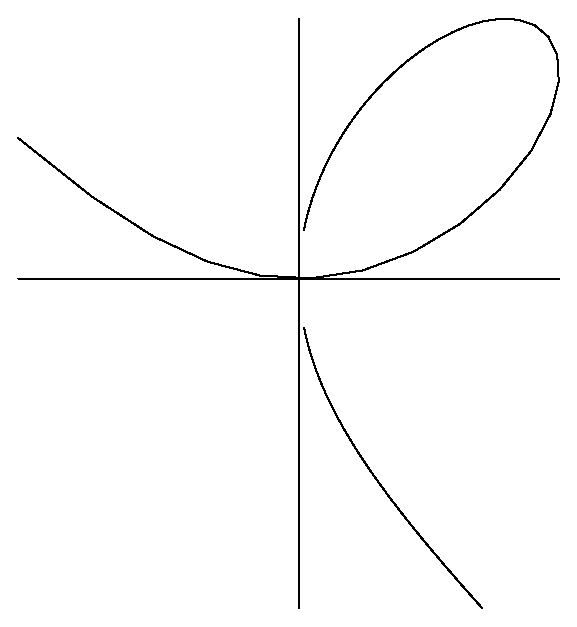
\includegraphics[width=7cm]{figure17.eps}
\caption{The Folium of Descartes}
\label{figure-folium}
\end{figure}

The folium is historically interesting because it was (as the
name suggests) studied by Descartes. He was concerned,
specifically, with the slope of the folium; this was a
question he couldn't answer with the mathematics of his day.
This question was answered by Newton in the following decades,
using the techniques of calculus. Let's follow in these steps
and calculate the slope of the folium.
\begin{align*}
\frac{dx}{dt} & = \frac{3(1+t^3) - 3t3t^2}{(1+t^3)^2} \\
\frac{dy}{dt} & = \frac{6t(1+t^3) - 3t^23t^2}{(1+t^3)^2} \\
\frac{dy}{dx} & = \frac{6t + 6t^4 - 9t^4}{3 + 3t^3 -
9t^3} = \frac{6t-3t^4}{3-6t^3} = \frac{2t-t^4}{1-2t^3}
\end{align*}
This slope is undefined when $t = \sqrt[3]{\frac{1}{2}}$. We
expect a vertical tangent there (this is the far edge of the
loop section of the folium).
\end{example}

\begin{example}
Let's calculate the slope of the logarithmic spiral. 
\begin{align*}
\gamma(t) & = (ae^{bt} \cos t, ae^{bt} \sin t) \\
\frac{dx}{dt} & = bae^{bt} \cos t - a e^{bt} \sin t \\
\frac{dy}{dt} & = bae^{bt} \sin t + ae^{bt} \cos t \\
\frac{dy}{dx} & = \frac{bae^{bt} \sin t + ae^{bt} \cos t} {
bae^{bt} \cos t - a e^{bt} \sin t} = \frac{b\sin t + \cos t}{b
\cos t - \sin t}
\end{align*}
This slope undefined when $b \cos t = \sin t$ or $b = \tan
t$. This is a regular occurence, but that makes sense, since
there are infinitely many locations on the curve where
we get a vertical tangent. This is $0$ similarly when $b =
-\cot t$, finding the infinitely many times where we get a
horizontal tangent. 
\end{example}

\subsection{Velocity and Distance on a Parametric Curve}
\label{velocity-distance}

Unlike loci, we can ask for the distance (length) of a
parametric curve. We're going to think in terms of
infinitesimals. 

\begin{defn}
The symbol $ds$ represents an infinitesimal distance along
the curve. We define $ds$ as the pythagorean combination of
$dx$ and $dy$, the infinitesimal distances in $x$ and $y$.
\begin{equation*}
ds = \sqrt{dx^2 + dy^2}
\end{equation*} 
\end{defn}

\begin{defn}
If this is distance, then the velocity along the curve is
its rate of change $\frac{ds}{dt}$. 
\end{defn}

With these two definition, we notice something important.
\begin{equation*}
ds = \sqrt{dx^2 + dy^2} \implies \frac{ds}{dt} = \sqrt{
\left( \frac{dx}{dt} \right)^2 + \left( \frac{dy}{dt}
\right)^2 }
\end{equation*}
This definition of $\frac{ds}{dt}$, motivated by
infinitesimals, will be our definition of velocity along a
parametric curve. Let's look at some examples.

\begin{example}
The curve $\gamma(t) = (t,t)$ has $\frac{ds}{dt} = \sqrt{1+1}
= \sqrt{2}$. This is a reasonable answer, since the linear
process moves along the curve at a constant rate of $\sqrt{2}$
units of distance per unit of time.
\end{example}

\begin{example}
The curve $\gamma(t) = (t^2,t^2)$ traces the same line,
but with speed $\frac{ds}{dt} = \sqrt{4t^2 + 4t^2} = 2\sqrt{2}
t$. In this quadratic behavior, speed increases with the
parameter and we have constant acceleration.
\end{example}

\begin{example}
The curve $\gamma(t) = \left(\frac{1}{t}, \frac{1}{t}
\right)$ traces the same line, but move towards the origin. It
has $\frac{ds}{dt} = \sqrt{\frac{1}{t^4} + \frac{1}{t^4}} =
\frac{\sqrt{2}}{t^2}$, which gets slower and slower. This
makes sense, since we have to have $t \rightarrow \infty$
before we get close to the origin. The movement along the
curve has to become very slow as $t$ increases.
\end{example}

\begin{example}
Recall the cycloid: $\gamma(t) = (a(t-\sin t),
a(1-\cos t))$. It has $\frac{dx}{dt} = a - a \cos t$ and
$\frac{dy}{dt} = a \sin t$, so we calculate its velocity.
\begin{align*}
\frac{ds}{dt} & = \sqrt{(a-a\cos t)^2 + a^2 \sin^2 t } \\
& = \sqrt{a^2 - 2a^2\cos t + a^2 \cos^2 t + a ^2 \sin^2 t} \\
& = \sqrt{a^2 - 2a^2 \cos t + a^2} = a\sqrt{2(1-\cos t)} 
\end{align*}
We can notice that $1-\cos t$ is always positive, so the square
root is well defined. Curiously, at $t=0$, $t=2\pi$ and
any other multiple of $2\pi$, we get no velocity.
\end{example}

We said in the previous section that the cycloid is the path
of a point on a wheel. When $t$ is a multiple of $2\pi$, the
point on the wheel is momentarily in contact with the ground
and its speed is zero. That means that on a rolling wheel, the
point touching the ground at any instant it momentarily
stationary. This is something to ponder the next time you
watch a train or other fast moving wheeled vehicle: at every
instant in time, there is at least one point on the vehicle
which isn't moving.

\subsection{Arclength}
\label{arclength}

We defined $ds = \sqrt{dy^2 + dx^2}$. We thought of this as
an infintesimal piece of distance along the curve. Therefore,
to get the entire distance along the curve, we need to add up
all the infinitesimal distance. Adding up infinitesimals is
the business of integration. 

\begin{defn}
The distance travelled along a parametric curve, as the
parameter goes from $t_0$ to $t_1$, is the integral of $ds$.
\begin{equation*}
L = \int ds = \int_{t_0}^{t_1} \sqrt{\frac{dx}{dt}^2
+\frac{dy}{dt}^2}dt 
\end{equation*}
The distance travelled along a parametric curve is typically
called the \emph{arclength}.
\end{defn}

\begin{example}
A very nice example is the circle: $\gamma(t) = (\cos t, \sin
t)$ for $t \in [0,2\pi]$. Its length is calculated by 
integration.
\begin{equation*}
L = \int_0^{2\pi} \sqrt{ \sin^2 t+ \cos^2 t}dt = \int_0^{2\pi}
dt = 2\pi
\end{equation*}
It is very good that we recover the known circumference
distance of a unit circle. However, there are other
parametrizations. 
Take $\gamma(t) = (\cos 3t, \sin 3t)$ for $t \in [0,
2\pi/3]$ and calculate the length. 
\begin{equation*}
L = \int_0^{\frac{2\pi}{3}} \sqrt{ 9\sin^2 3t+ 9\cos^2 3t}dt =
\int_0^{\frac{2\pi}{3}} 3 dt = \frac{2\pi}{3} 3 = 2\pi
\end{equation*}
Happily, we still get the same result.
\end{example}

\begin{example}
Let's reutrn to the cycloid $\gamma(t) =
(t-\sin t, 1-\cos t)$. The derivatives are $x^\prime = 1-\cos
t$ and $y^\prime = \sin t$. 
\begin{align*}
L & = \int_0^{2\pi} \sqrt{(x^\prime)^2 + (y^\prime)^2 } dt \\
& = \int_0^{2\pi} \sqrt{1 - 2\cos t + \cos^2 t + \sin^2 t} dt \\
& = \int_0^{2\pi} \sqrt{2 - 2\cos t} dt = \sqrt{2} \int_0^{2\pi}
\sqrt{1 - \cos t} dt \\
& = \sqrt{2} \int_0^{2\pi} \sqrt{2} \sqrt{\sin^2 \frac{t}{2}} dt 
= 2 \int_0^{2\pi} \left| \sin \frac{t}{2} \right| dt \\
& = 2 \int_0^{2\pi} \sin \frac{t}{2} dt 
= 2 2 \left. \left( - \cos \frac{t}{2} \right) \right|_0^{2\pi}
= 4( \cos 0 - \cos \pi) = 4 \cdot 2 = 8
\end{align*}
\end{example}

\begin{example}
An interesting example is the perimeter of an ellipse. It's
an impotant calculation historically, since it can determine
the length of elliptical orbits (among other applications). 
Let $a$ be the major (x) semiaxis and $b$ be the minor (y)
semiaxis. Then $\gamma(t) = (a \cos t, b \sin t)$ for $t \in
[0,2\pi]$ describes the ellipse. 

Before calculating, it is convenient to also define a new
quantity: the eccentricity of the ellipse. This is defined as
$e = \frac{\sqrt{a^2-b^2}}{a}$ (assuming that $a\geq b$) and
it always a number in $[0,1)$. Eccentricity is a nice way of
measuring how close an ellipse is to a circle. If $e = 0$ then
$a=b$ and we have a circle. As $e \rightarrow 1$ the ellipse
becomes narrower and narrower. Then we (try to) calculate the
length of the ellipse.

\begin{align*}
L & = \int_0^{2\pi} \sqrt{ (x^\prime)^2 + (y^\prime)^2} dt \\
& = \int_0^{2\pi} \sqrt{ a^2 \cos^2 t + b^2 \sin^2 t} dt \\
& = \int_0^{2\pi} \sqrt{ a^2 \sin^2 t + (b^2 - a^2) \sin^2 t +
a^2 \cos^2 t } \\
& = \int_0^{2\pi} a\sqrt{ 1 + \frac{b^2-a^2}{a^2} \sin^2 t} \\
& = a \int_0^{2\pi} \sqrt{ 1 - \frac{a^2 - b^2}{a^2} \sin^2 t} \\
& = a \int_0^{2\pi} \sqrt{ 1 - e^2 \sin^2 t}dt 
\end{align*}

If $e=1$, then we could use $1 - \sin^2 t = \cos^2 t$ and have
an easy integral. In this form, however, the integration is
very difficult. This is so difficult, in fact, that it has a
special name: this is an elliptic integral of the second kind.
These integrals have been studied for three hundred years, and
with good cause, since they have no elementary
anti-derivatives. Even without an elementary anti-derivative,
the behaviour can be investigated. This has led to many
insights in geometry; the notion of elliptic curves relates to
this integral and gives elliptic curves their names. 
\end{example}

\begin{example}
Another important special case is a parametric description of
the graph of a function. If $f(x)$ is defined on $[a,b]$, then
for $t \in [a,b]$ its graph can be written $\gamma(t) = (t,
f(t))$.
\begin{equation*}
L = \int_a^b \sqrt{1 + (f^\prime(t))^2}dt 
\end{equation*}
This is a convenient formula to have, since calculating the
lengths of graphs of function is a common activity.
\end{example}

\subsection{Independence of Parametrization}
\label{independence-parametrization}

The previous examples of the length of the circle raises an
important issue. Notions like distance should be intrinsic
to the \emph{shape}, not the rate of movement along the shape.
With parametric objects, we have to distinguish between that
which depends on the parameter (like velocity) and that which
is intrinsic to the shape (like arclength). For the
latter, we have to make sure that if we use a parametrization
to calculate an intrinsic quantity, the result is independent
of the parametrization.

In this case, the proof that distance is independent of
parametrization is simply accomplished by the substitution
rule for integrals. Let $\gamma(t)$ be a curve. Any other
parametrization can be achieved by a monotonoic function $t =
t(s)$ via reparametrization. If the original bounds of $t$
are $t_0$ and $t_1$, then choose $s_0$ and $s_1$ so that
$t(s_0) = t_0$ and $t(s_1) = t_1$. Then we're going to use the
substitution $t = t(s)$ with $dt = t^\prime(s) ds$ to change
the integral. 
\begin{align*}
L(t) & = \int_{t_0}^{t_1} \sqrt{ \frac{dx(t)}{dt}^2 +
\frac{dy(t)}{dy}^2} dt \\
& = \int_{t_0}^{t_1} \sqrt{ \frac{dx(t)}{dt}^2 +
\frac{dy(t)}{dy}^2} \frac{dt}{ds} \frac{dt}{\frac{dt}{ds}} \\
& = \int_{t_0}^{t_1} \sqrt{ \left( \frac{dx(t(s))}{dt}
\frac{dt}{ds} \right)^2 +\left( \frac{dy(t(s))}{dt}
\frac{dt}{ds} \right)^2} \frac{dt}{\frac{dt}{ds}} \\
& = \int_{s_0}^{s_1} \sqrt{\frac{dx(t(s))}{ds}^2 +
\frac{dy(t(s))}{ds}} ds = L(s)\\
\end{align*}
The substitution shows that the length doesn't depend on which
parametrization we use.

\subsection{Parametrization by Arclength}
\label{parametrization-arclength}

The issue of many parametrizations of the same shape is vexing.
If we want to work with intrinsic information, we always have
to deal with the different parametrizations. It would be very
convenient to have one special parametrization to choose.
Fortunately, such a parametriztion exists (or is chosen by
mathematicians). 

\begin{defn} 
The \emph{parametrization by arclength} is the parametrization
where $\frac{ds}{dt} = 1$, i.e., the unique parametrization
where we always move along the curve with speed of one unit of
distance per unit of time. To make it completely unique, we
also start the parameter at 0.
\end{defn}

The reason for the name is that the parameter can be
interpreted as the length along the curve. If we always cover
distance at a rate of one unit of distance per unit of time,
then after $t$ units of time we've covered $t$ units of
distance, for all choices of the parameter $t$. Therefore, it
is approprate to treat the parameter $t$ as the distance
covered. For this reason, we often write $s$ for this
parameter and we call $s$ the arclength parameter.

In order to construct this parametrization, we need a new
function: the arclength function. We need to be very careful
with variables when defining this function. Let $\gamma(t)$ be
our parametric curve. We're going to introduce a new variable
$u$, which will also act as the parameter. The reasons for
this $u$ is that we need an internal variable for the
arclength integral.

\begin{defn} 
\begin{equation*}
s(t) = \int_a^t \sqrt{(x^\prime(u))^2 + (y^\prime(u))^2} du 
\end{equation*}
This $s(t)$ is the arclength function. It depends on the parameter
$t$ and starts at $t=a$. Since $t$ is outside the integral,
we needed the temporary variable $u$ to do the integration.
The arclength function measure how much length we've covered
as the parameter goes from the start $a$ to $t$. 
\end{defn}

The arclength function is guaranteed to be an increasing
function, since it is an integral of a positive function.
Therefore it is invertible. It also starts at 0, $s(a) = 0$.
The maximum value of $s$ is $s(b) = L$, the total length of
the curve. Therefore, we can write the inverse as $t(s)$
where $s \in [0, L]$. Then we can substitute $t(s)$ for $t$
to get $\gamma(t(s))$, a reparametrization.

What has this accomplished? We've turned the arclength
function into the parameter. Therefore, this is the
parametrization by arclength. It is the unique parametrization
with speed one, where the parameter and length along the curve
are always the same. 

\begin{example}
Here's the process for parametrizing a circle of radius $4$ by
arc-length.
\begin{align*}
\gamma(t) & = (4 \cos t, 4 \sin t) \hspace{2cm} t \in [0, 2\pi] \\
s(t) & = \int_0^t \sqrt{(x^\prime(u))^2 + (y^\prime(u))^2} du \\
& = \int_0^t \sqrt{16 \sin^2 u + 16 \cos^2 u} du \\
& = \int_0^t 4 du \\
s(t) & = 4t \\
t(s) & = \frac{s}{4} \\
t & = 0 \implies s = 0 \\
t & = 2\pi \implies s = 8\pi \\
\gamma(s) & = \left(4 \cos \frac{s}{4}, 4 \sin \frac{s}{4}
\right) \hspace{2cm} t \in [0,8\pi]
\end{align*}
\end{example}

\section{Volumes}
\label{volumes}

\subsection{Volumes by Cross-Sectional Slices}
\label{cross-sectional-slices}

For parametric curves, we approached the length of a curve by
defining an infinitesimal length $ds$ and then using
integration to `add up' all the infinitesimals.
\begin{equation*}
L = \int ds
\end{equation*}
This technique of thinking in infinitesimals is useful for
many applications of integration. In this section, we're going to
use it to calculate volumes.

\begin{example}
A basic example is the volume of a sphere. In these
infinitesimal arguments, we need to divide the object into
pieces, either slices or more complicated shapes, which have
an infinitesimal thickness. For the sphere, we divide it into
infinitesimally thin discs. Let's say the sphere of radius $r$
is centered at the origin in $\RR^3$. We slice it into
vertical slices with circular cross sections.

What is the radius of each
disc? If we look at a cross-section of the middle of the
sphere, we get the circle $x^2 + y^2 = r^2$. If our slices
are vertical, then their radius is simply the $y$ value $y =
\sqrt{r^2 - x^2}$. Then, as we move from $x = -r$ to $x = r$,
we get all the radii from $0$ to $r$ and back to $0$ again.
All of these discs have thickness $dx$, an infinitesimal, and
area $\pi y^2 = \pi (r^2 - x^2)$. Then we just add up all the
infinitesimal pieces in an integral.
\begin{align*}
V & = \int_{-r}^r A dx = \int_{-r}^r \pi (r^2 - x^2) dx \\
& = \pi \int_{-r}^r r^2 - x^2 dx = \left. \pi r^2 x - \pi
\frac{x^3}{3} \right|_{-r}^r \\
& = \pi r^3 - (-\pi r^3) - \left( \frac{\pi r^3}{3} +
\frac{\pi r^3}{3} \right) = 2\pi r^3 - \frac{2\pi r^3}{3} =
\frac{4\pi r^3}{3}
\end{align*}
The result is the conventional old formula for the volume of a
sphere. 
\end{example}

\begin{figure}[t]
\centering

\includegraphics[width=7cm]{figure18.eps}
\caption{Slices of the Sphere}
\label{figure-slices-sphere}
\end{figure}

\begin{figure}[t]
\centering
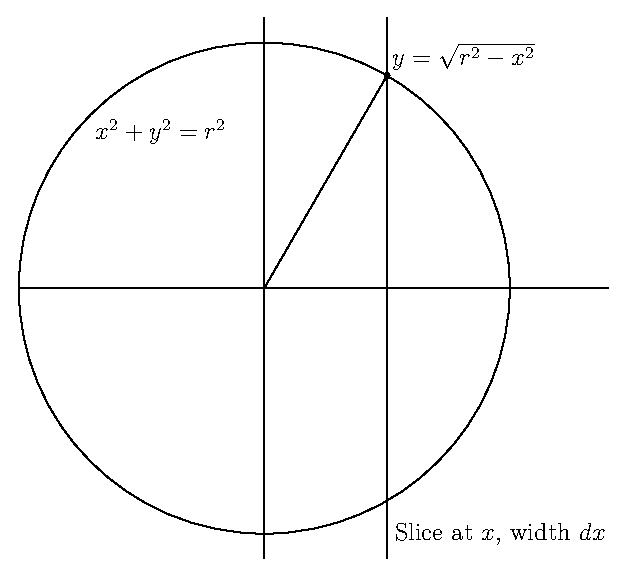
\includegraphics[width=8cm]{figure19.eps}
\caption{Cross Section of a Sphere}
\label{figure-cross-secdtion-sphere}
\end{figure}

\begin{figure}[ht]
\centering
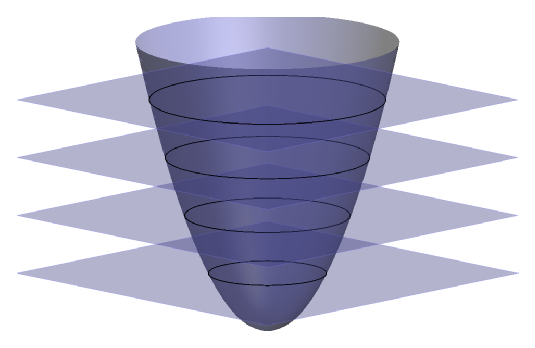
\includegraphics[width=9cm]{figure20.eps}
\caption{Slices of a Parabaloid}
\label{figure-slices-parabaloid}
\end{figure}

\begin{example}
A slightly more involed example is the volume of a parabaloid of
height $h$ and radius $a$. The parabaloid is described by the
function $y = h \left(\frac{x}{a}\right)^2$ rotated around the
$y$ axis. We have $x \in [0, a]$ and $y \in [0, h]$. (Many of
these volume problems can be expressed as surfaces of
revolution: take a function and revolve it around a axis.) To
add up the slices, we move in the $y$ direction. At each $y$
the radius is $x = a\sqrt{\frac{y}{h}}$. The area is $\pi x^2
= \frac{\pi a^2 y}{h}$ and the thickness is $dy$.
\begin{align*}
V & = \int_0^h \pi a^2 \frac{y}{h} dy = \frac{\pi a^2}{h}
\int_0^n y dy \\
& = \frac{\pi a^2 h^2}{2h} = \frac{\pi a^2 h}{2}
\end{align*}
We get a volume equation which is similar to a cone
$\left(\frac{1}{3} \pi r^2 h\right)$ but divided by $2$
instead of $3$.
\end{example}

\subsection{Volumes by Spherical or Cylindrical Shells}
\label{shells}

In the previous section, we used cross-sectional slices,
slicing with a plane to produce the circles. However, there
are other ways to slice up a volume. In this section, we look
at the general method of shells. Instead of slicing with a
plane, we think of a volume as a nested collection of similar
shapes called shells. You could think of the (rough) spheres
that form an onion, or stacking Matryoshka dolls. 

If we think of the shells as infinitesimally thin, with
thickness $dr$, then we can add up all the infinitesimal
volumes of the shells just as with did with slices in the
previous section. We use $dr$ as the infinitesimal thickness,
since we often arrange the shells in a radial direction.

Our examples in this section will use cylindrical shells. If
we have a cylinder with radius $r$ and height $h$, its surface
area is $A = 2\pi r h$. A cylindrial shell will have
thickness $dr$, so infinitesimal volumes is $dV = 2\pi r h dr$.
To find a volume, we express $h$ as a function of $r$, and
integrate.

\begin{example}
For an example, consider a pottery bowl whose cross section is
roughly the area between $x^2$ and $x^4$ on the interval
$[-1,1]$. 

\begin{figure}[ht]
\centering
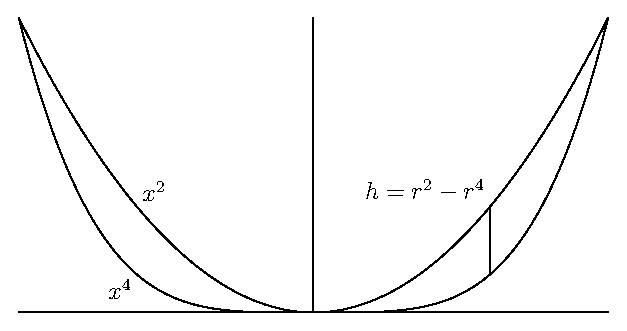
\includegraphics[width=9cm]{figure21.eps}
\caption{Cross Section of a Bowl}
\label{figure-cross-section-bowl}
\end{figure}

Sliced into cylindrial shells, each shell has height $h = r^2
- r^4$, based on the radius $r$ from the centre of the bowl.
\begin{align*}
V & = \int_0^1 2\pi r (r^2 - r^4) dr \\
& = 2\pi \int_0^1 r^3 - r^5 dr \\
& = \left. 2\pi \left( \frac{r^4}{4} - \frac{r^6}{6} \right)
\right|_0^1\\
& = \left. 2\pi \left( \frac{3r^4 - 2r^6}{12} \right) \right|_0^1 =
\frac{2\pi}{12} = \frac{\pi}{6} 
\end{align*}
\end{example}

\begin{example}
A second example is a bell which is the surface of revolution
about the $y$ axis of the function $e^{-x^2}$ between $[-2,2]$. 

\begin{align*}
V & = \int_0^2 2\pi re^{-r^2} dr \\
u & = e^{-r^2}\\
du & = -2r e^{-r^2} dr \\
u(0) & = 1 \\
u(2) & = \frac{1}{e^4} \\
V &= \int_1^{\frac{1}{e^4}} -\pi du = \left. -\pi u
\right|_1^{\frac{1}{e^4}} = \pi \left( 1 - \frac{1}{e^4}
\right) = \pi \frac{e^4-1}{e^4} 
\end{align*}
\end{example}

\begin{figure}[h]
\centering
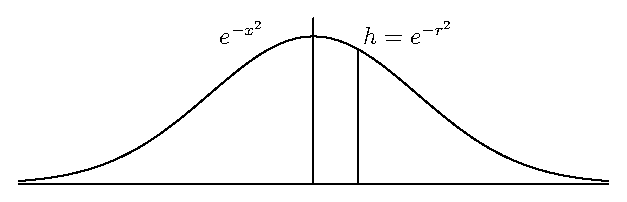
\includegraphics[width=9cm]{figure22.eps}
\caption{Cross Section of a Bell}
\label{figure-cross-section-bell}
\end{figure}

\begin{example}
The Horn of Gabriel is a surface of revolution under the graph
of $f(x) = \frac{1}{x}$ for $x \in [1,\infty)$. We can use an
improper integral to calculate its volume.
\begin{equation*}
V = \int_1^\infty \pi \frac{1}{x^2} = \lim_{a \rightarrow
\infty} \int_1^a \frac{\pi}{x^2} = \lim_{a \rightarrow \infty}
\left. \frac{-\pi}{x} \right|_1^a = \lim_{a \rightarrow
\infty} \frac{-\pi}{a} + \pi = \pi
\end{equation*}
The volume is finite! Even though the Horn of Gabriel extends
to infinity, it narrows quickly enough that it only contains a
finite volume.
\end{example}

\begin{example}
An interesting example is the calculation of the volume of a
torus. A torus is defined by a larger radius $a$, which is
the distance from the centre of the torus to the centre of any
cross-sectional circle, and a smaller radius $b$, which is the
radius of any cross-sectional circle.

\begin{figure}[ht]
\centering
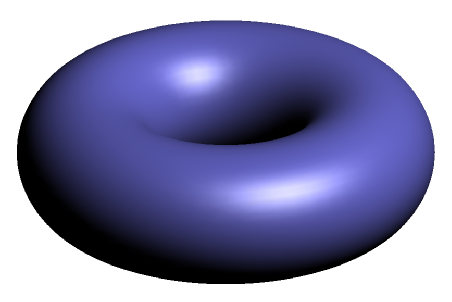
\includegraphics[width=8cm]{figure23.eps}
\caption{A Torus}
\label{figure-torus}
\end{figure}

The cross section of a torus consists of two circles.

\begin{figure}[ht]
\centering
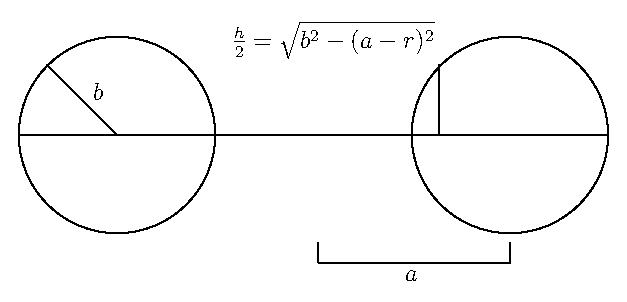
\includegraphics[width=8cm]{figure24.eps}
\caption{A Cross-Section of a Torus}
\label{figure-cross-section-torus}
\end{figure}

When we take a cross section, we get the circle $(x-a)^2 + y^2
= b^2$. We can solve for $y = \sqrt{b^2 - (x-a)^2}$. This is
only half the height of a cylindrical shell, so $h = 2y$. Then
$x$ is the radius, so we can write $h = 2 \sqrt{b^2 -
(r-a)^2}$ We will integrate from $a-b$ to $a+b$ in $r$, to
cover one of the cross-sectional circles.

\begin{align*}
V & = 2 \int_{a-b}^{a+b} 2\pi r \sqrt{b^2 - (r-a)^2} dr \\
u & = r-a \implies r = u+a\\
du & = dr \\
u(a-b) & = -b \\
u(a+b) & = b \\
V & = 4\pi \int_{-b}^b (u+a) \sqrt{b^2 - u^2} du \\
& = 4\pi \left[ \int_{-b}^b u \sqrt{b^2-u^2} du + \int_{-b}^b a
\sqrt{b^2-u^2} du \right] \\
\int_{-b}^b u \sqrt{b^2-u^2}du & = \left. \frac{1}{-2}
\frac{2}{3} (b^2 -u^2)^{\frac{3}{2}} \right|_{-b}^b = 0 \\
\int_{-b}^b \sqrt{b^2 - u^2} & - \int_{-\pi/2}^{\pi/2} |b\cos
\theta| b \cos \theta d\theta \\
u & = b \sin \theta \\
du & = b \cos \theta d \theta \\
u = b & \implies \theta = \frac{\pi}{2} \\
u = - b & \implies \theta = - \frac{\pi}{2} \\
\int_{-b}^b \sqrt{b^2 - u^2} & = \int_{-\pi/2}^{\pi/2} |b\cos
\theta| b \cos \theta d\theta \\
& = b^2 \int_{-\pi/2}^{\pi/2} \frac{1 + \cos 2\theta}{2} d
\theta \\
& = b^2 \int_{-\pi/2}^{\pi/2} \frac{1}{2} d\theta+ b^2
\int_{-\pi/2}^{\pi/2} \frac{\cos 2\theta}{2} d\theta \\
& = \frac{b^2}{2} \left( \frac{\pi}{2} - \frac{-\pi}{2} \right) + 0 \\
& = \frac{b^2\pi}{2} \\
V & = 4\pi \left[ 0 + \frac{b^2 \pi}{2} \right] = 2\pi^2 a^2 b
\end{align*}
Therefore, the volume of a torus with major radius $a$ and
minor radius $b$ is $2\pi^2 a^2 b$. As a curious obvservation,
we can write this as $(2\pi a)(\pi b^2)$. The $2\pi a$ factor
is the circumference of the large circle with radius $a$,
which lies at the center of each cross-sectional circle. The
$\pi b^2$ factor is the radius of each cross-sectional circle.
Therefore, the torus has the same volume of a cylinder with
height equal to this circumference and radius $b$.
\end{example}

\section{Surface Areas}
\label{surface-areas}

We have been calculating the volumes of surfaces of
revolution: objects formed by taking a graph or locus and
spinning its around an axis. In this section, we expand the
process to also calculate surface areas.

Let's say that our surface is formed by rotating $f(x)$ around
the $x$ axis on a domain $x \in [a,b]$. Then $f(x)$ is the
radius of the surface as we move in the $x$ direction. To
calculate surface area, we seperate the surface of revolution
into tiny cylindrical shells of radius $f(x)$. When we worked
with slices for volume, the width of a slice was $dx$, and
simple infinitesimal. For surface area, this doesn't capture
the complete behaviour. 

We look at the lengths of parametric curves for inspiration.
If we call $ds$ the infinitemisal width of a cylinder of
surface area, then $ds = \sqrt{ 1 + (f^\prime(x))^2}dx$. 

\begin{figure}[h]
\centering
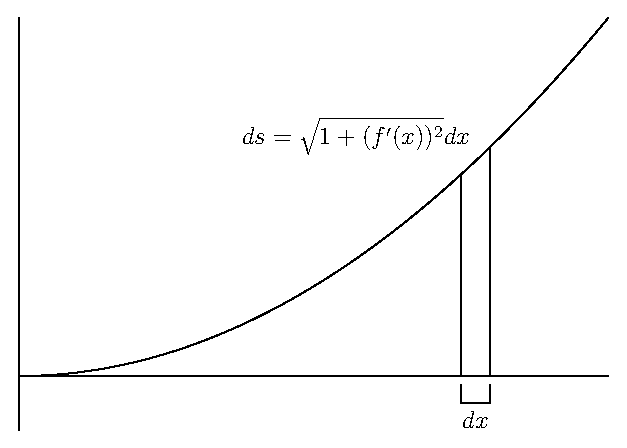
\includegraphics[width=7cm]{figure25.eps}
\caption{The Width $ds$ of a Piece of Surface Area}
\label{figure-piece-surface-area}
\end{figure}

Then the area of each infinitesimal cylinder is circumference
times width. 
\begin{equation*}
dA = 2\pi f(x) dx = 2\pi f(x) \sqrt{ 1 + (f^\prime(x))^2} dx
\end{equation*}
The surface area calcluation is the integral of these
infinitesimal pieces.
\begin{equation*} 
A = \int_a^b 2\pi f(x) \sqrt{1 + (f^\prime(x))^2} dx 
\end{equation*}

\begin{example}
A classic example is the surface area of a sphere. The sphere
is a surace of revolution for $f(x) = \sqrt{r^2-x^2}$ for $x
\in [-r,r]$. 
\begin{align*}
A & = 2 \int_0^r 2\pi \sqrt{r^2-x^2} \sqrt{ 1+ \frac{x^2}{r^2 -
x^2}} dx \\
& = 4 \pi \int_0^r \sqrt{ r^2 - x^2 + x^2} dx = 4\pi
\int_0^r r dx \\
& = \left. 4 \pi r x \right|_0^r = 4 \pi r^2
\end{align*}
\end{example}

\begin{example}
We can also calculate the surface are of a cone of height $h$
and radius $r$. This is a surface of revolution of the
function $y = \frac{r}{h} x$ for $x \in [0, h]$. 
\begin{align*}
A & = \int_0^h 2\pi \frac{r}{h} x \sqrt{ 1 + \frac{r^2}{h^2}} dx
\\
& = 2\pi \frac{r}{h} \sqrt{1 + \frac{r^2}{h^2}} \int_0^h x dx \\
& = 2\pi \frac{r}{h} \sqrt{1 + \frac{r^2}{h^2}} {h^2}{2} \\
& = \pi r \sqrt{h^2 + r^2} 
\end{align*}
\end{example}


\begin{example}
We could also revolve a graph around the $y$ axis.
If we do this, we have to write to have $x = f(y)$ instead of $y = f(x)$.
For example, the parabaloid $y = \frac{h}{a^2} x^2$ with height
$h$ and radius $a$ has $x = a \sqrt{\frac{y}{h}}$, so we can
find its surface area by integrating in the variable $y$.
\begin{align*}
A & = \int_0^h 2\pi a \sqrt{\frac{y}{h}} \sqrt{ 1 +
\frac{a^2}{4yh}} dy \\
& = 2\pi a \int_0^h \sqrt{ \frac{y}{h} + \frac{a^2}{4h^2}} \\
& = \left. 2\pi a \left(\frac{y}{h} + \frac{a^2}{4h^2}
\right)^{\frac{3}{2}} \frac{2}{3} h \right|_0^h \\
& = \frac{4\pi ah}{3} \left(1 + \frac{a^2}{4h^2} =
\right)^{\frac{3}{2}} \\
& = \frac{a\pi}{3} \left( 4h^2 + a^2 \right)^{\frac{3}{2}}
\end{align*}
\end{example}

\begin{example}
The Horn of Gabriel had finite volume even though it was
arbitrarily long. What is its surface area?
\begin{align*}
A & = \int_1^\infty 2\pi \frac{1}{x} \sqrt{ 1 + \frac{1}{x^4}}
dx \geq 2 \pi \int_0^\infty \frac{1}{x} dx = \infty 
\end{align*}
By asymptotic analysis on the integrand, we see this will
never converges. The horn of gabriel is an object with finite
volume and infinite surface area.
\end{example}

\begin{example}
Lastly, we can calculate the surface area of the exponential
bell. This is the surface of revolution for $f(x) = e^{x}$
on the domain $x \in [0, a]$. 
\begin{align*}
A & = \int_0^1 2\pi e^x \sqrt{1 + e^{2x}} dx \\
u & = e^x \\
du & = e^x dx \\
u(0) & = 1 \\
u(a) & = e^a \\
A & = 2\int_1^{e^a} \sqrt{1+u^2} du \\
u & = \tan \theta \\
du & = \sec^2 \theta d \theta \\
A & = \int_{u=1}^{u=e^a} \sec^3 \theta d \theta \\
& = \int_{u=1}^{u=e^a} \frac{\cos \theta}{(1-\sin^2 \theta)^2}
\theta d \theta \\
& = \left. \arctanh \sin \theta \right|_{u=1}^{u=e^a} \\
& = \left. \arctanh \left( \sqrt{1 - \frac{1}{\sec^2 \theta}}
\right) \theta \right|_{u=1}^{u=e^a} \\
& = \left. \arctanh \left( \sqrt{1 - \frac{1}{u^2}}
\right) \theta \right|_{u=1}^{u=e^a} \\
& = \arctanh \left( \sqrt{1 - e^{-2a}} \right) -\arctanh 0 \\
& = \arctanh \left( \sqrt{1 - e^{-2a}} \right) 
\end{align*}
This is not a particularly nice forumla, but it does give the
surface area.
\end{example}

\section{Probability}
\label{probability}

\subsection{Probability Density Functions}
\label{density-functions}

The final major application of integration in this chapter is
the use of integration to understand continuous probability.
When dealing with probability, there are two major kinds of
data: discrete and continuous. In discrete data, there are a
finite number of seperate possible measurements, each of which
has a finite probability. The study of discrete probability
can be entirely accomplished with finite sums (though even
there, caluculus can give surprising insights.)

Continuous probability involves measurements which can vary
anywhere within a range. Test scores are a typical discrete
measurement: there are only a finite number of test results.
Heights in a population are a typical continuous measurement:
assuming sufficient precision, a height can be any real number
in a particular range. At least mathematically, there are
infinitely many possible measurements. As opposed to discrete
probability, we can't assign a specific likeliness to any
particular measurement in a continuous situation. Instead, we
can assign a probability to a range of measurements. For
example: there is a 20\% change that an adult female caribou
stands more than 125 cm tall at the shoulder.

\begin{defn}
A \emph{probability density} is defined to be an integrable function
$f(x) : [a,b] \rightarrow [0, \infty)$ such that
\begin{equation*}
\int_a^b f(x) dx = 1.
\end{equation*}
\end{defn}

The interval $[a,b]$ is the range of all possible measurements.
The integral condition is simply saying that all measurements
fall in this range (with probability 1). Then, if we have
$x_0$ and $x_1$ in the interval $[a,b]$, the probability of a
measurement between $x_0$ and $x_1$ is given by the integral
of the density.
\begin{equation*}
\int_{x_0}^{x_1} f(x) dx
\end{equation*}
We need the probability density function to be positive
because negative probability doesn't make any sense. 
Note that measurements are $x$ values -- inputs to the
function, not outputs. $f(x)$ measures, in some sense, the
likeliness of $x$ being a measurement. In the ensuing study
of probability, all information about the situation
is determined from the probability density function.

Since it is a common convention, we will also refer to the
probability density function as a \emph{probability
distribution} or simply a distribution.

\subsection{Normalization}
\label{normalization}

Often we are given a positive function $f(x)$ on an interval,
but not necessarily with the condition that its integral over
the interval is one. We can choose parameters or
multiply $f(x)$ by some constant to ensure that the total
integral over the interval is one; such a process is called
normalization. 

\begin{example}
Let $\alpha > 0$ and $f(x) = e^{-\alpha x}$. We consider
$f(x)$ a possible density function on $[0, \infty)$. We try to
calculate its integral over this whole interval.
\begin{align*}
\int_0^\infty e^{-\alpha x} dx & = \lim_{a \rightarrow \infty}
\int_0^a e^{-\alpha x} dx \\
& = \lim_{a \rightarrow \infty} \left. \frac{e^{-\alpha
x}}{-\alpha} \right|_0^a \\
& = \lim_{a \rightarrow \infty} \frac{-e^{-\alpha a}}{\alpha} +
\frac{1}{\alpha} = \frac{1}{\alpha} 
\end{align*}
We must have a total integral of $1$ for $f$ to be a
probability density function, which means that $\alpha = 1$.
$f(x) = e^{-x}$ is a probability density function on
$[0,\infty)$. This interval means that all possible postiive
values are measurements. The fact that $f$ is a decay
function means that measurements gets less and less likely as
values get large. The probability of an event between $0$ and
$1$ is 
\begin{equation*}
\int_0^1 e^{-x} dx = \left. e^{-x} \right|_0^1 = -e^{-1} + 1 = 1 -
\frac{1}{e} \doteq 0.632.
\end{equation*}
Likewise, the probability of a measurement bewteen $1$ and
$2$ is 
\begin{equation*}
\int_1^2 e^{-x} dx = \left. e^{-x}\right|_1^2 = -e^{-2} +
\frac{1}{e} = \frac{1}{e} - \frac{1}{e^2} = \frac{e-1}{e^2}
\doteq 0.233.
\end{equation*}
\end{example}

\begin{figure}[ht]
\centering
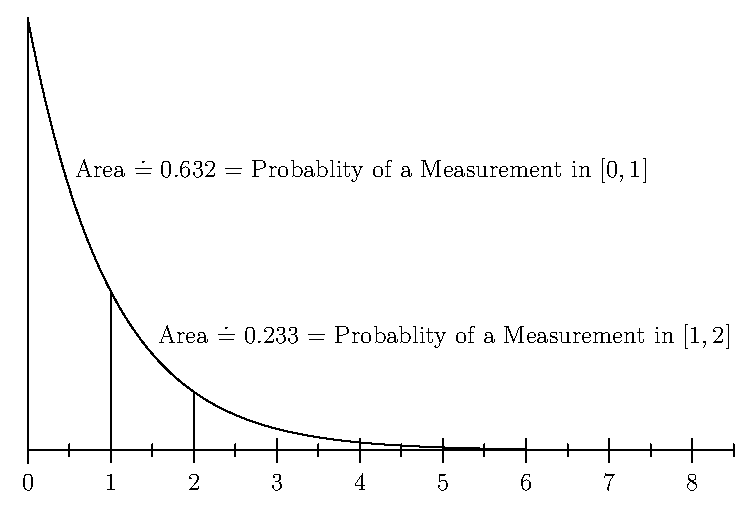
\includegraphics[width=12cm]{figure27.eps}
\caption{The Probability Density $e^{-x}$}
\label{figure-probability-density}
\end{figure}

\begin{example}
The most well-known probability density function is the
bell curve, which is also called the gaussian distribution or
normal distribution. In full generality it depends on two
parameters $\mu$ and $\sigma$ and has the following form.
\begin{equation*}
f(x) = \frac{1}{\sigma \sqrt{2\pi}}
e^{-\frac{(x-\mu)^2}{2\sigma^2}}
\end{equation*}
First, let's consider $f(x) = e^{-x^2}$ and try to normalize.
\begin{equation*}
\int_{-\infty}^\infty e^{-x^2} dx 
\end{equation*}
This is a problematic integral: $e^{-x^2}$ has no elementary
anti-derivative. The value of the integral is calculuced by
clever techniques in multi-variable calculus; for us, we'll
just state the value.
\begin{equation*}
\int_{-\infty}^\infty e^{-x^2} dx = \sqrt{\pi}
\end{equation*}
This allows normalization. $f(x) =
\frac{1}{\sqrt{\pi}} e^{-x^2}$ is a probability distribution on
all of $\RR$. 
\end{example}

\begin{figure}[ht]
\centering
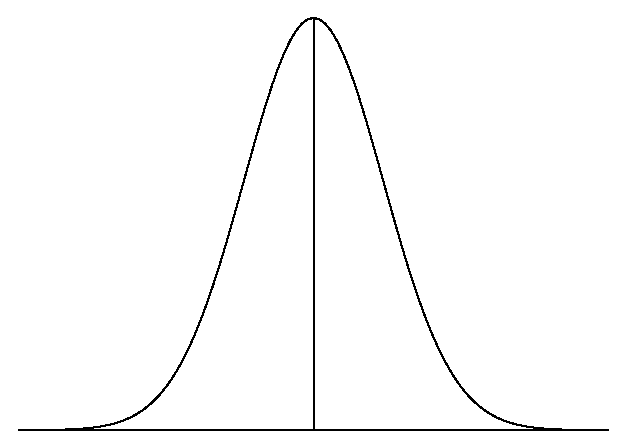
\includegraphics[width=9cm]{figure26.eps}
\caption{The Gaussian Distribution $\frac{1}{\sqrt{\pi}}
e^{-x^2}$}
\label{figure-gaussian-distribution}
\end{figure}

\begin{example}
Here is another common and important example.
\begin{equation*}
f(x) = \left\{ \begin{matrix} A & x \in [a,b] \\ 0 & x \notin
[a,b] \end{matrix} \right.
\end{equation*}
This measure an equal probablity of all measurements in the
range $[a,b]$. It is normalized by setting $A = \frac{1}{b-a}$. 
\end{example}

\subsection{Means}
\label{means}

For discrete probability, a mean or average of the expected
measurements is relatively intuitive: we just add up the
measurements multiplied by their probabilities. What a
mean should be for a continuous probability isn't as
immediately obvious, since we can't add up the
infinitely-many measurements. However, we can still take
inspiration from the discrete case. 

Let's consider finite probability for a moment. Say that there
are $n$ events with probabilities $p_i$ and measurements
$r_i$. Then the normalization is
\begin{equation*}
\sum_{i=1}^n p_i = 1.
\end{equation*}
The mean is the sum of the measurements multiplied by their
probabilities.
\begin{equation*}
\sum_{i=1}^n r_i p_i
\end{equation*}
These discrete calculations give inspiration for the
continuous case. The major difference, for continuous
probability, is that our sums are now integrals. Apart from
the difference, we still basically take the same steps:
multiply by the measurement to get the mean. 

\begin{defn}
The average or mean of a probability density $f(x)$ on $[a,b]$
is defined to be the following integral. 
\begin{equation*}
\mu = \int_a^b x f(x) dx
\end{equation*}
\end{defn}

\begin{example}
For $f(x) = e^{- x}$ on $[0, \infty)$, this is
the mean calculation (using integration by parts).
\begin{align*}
\mu & = \int_0^\infty x e^{-x} dx \\
& = \left. - x e^{-x} \right|_0^\infty + \int_0^\infty
e^{-x} dx \\
& = 0 + \left. e^{-x} \right|_0^\infty = 1
\end{align*}
This mean makes some sense for a decay function. Even though very
large measurements are possible, they become very unlikely.
The most likely measurements are near $0$, so the mean works
out to $1$.
\end{example}

\begin{example}
Let's also calculate the mean for $\frac{1}{b-a}$ (constant
probability on the interval $[a,b]$).
\begin{align*}
\mu & = \int_a^b \frac{1}{b-a} x dx \\
& = \left. \frac{1}{b-a} \frac{x^2}{2} \right|_a^b \\
& = \frac{b^2-a^2}{2(b-a)} = \frac{b+a}{2}
\end{align*}
The mean is exactly halfway between the endpoints. Since
the probability is constant, this makes perfect sense.
\end{example}

\begin{example}
Let's calculate the mean for the normal distribution in
full detail, using the parameters $\mu$ and $\sigma$. 
\begin{align*}
f(x) & = \frac{1}{\sigma
\sqrt{2\pi}}e^{-\frac{(x-\mu)^2}{2\sigma^2}} \\
\mu & = \int_{-\infty}^\infty
\frac{xe^{-\frac{(x-\mu)^2}{2\sigma^2}}}{\sigma \sqrt{2\pi}} dx
\\
& v = x-\mu \\
& = \int_{-\infty}^\infty
\frac{(v+\mu)e^{-\frac{v^2}{2\sigma^2}}}{\sigma \sqrt{2\pi}} dx \\
& = \int_{-\infty}^\infty
\frac{(v)e^{-\frac{v^2}{2\sigma^2}}}{\sigma \sqrt{2\pi}} dx 
+ \int_{-\infty}^\infty
\frac{(\mu)e^{-\frac{v^2}{2\sigma^2}}}{\sigma \sqrt{2\pi}} dx \\
& = 0 + \frac{\mu}{\sigma \sqrt{2\pi}} \int_{-\infty}^\infty
e^{-\frac{v^2}{2\sigma^2}} dx \\
w & = \frac{v}{\sigma \sqrt{2}} \\
& = \frac{\mu}{\sigma \sqrt{2\pi}} \sigma \sqrt{2} \int_{-\infty}^\infty
e^{-w^2} dw = \frac{\mu}{\sqrt{\pi}} \sqrt{\pi} = \mu 
\end{align*} 
The mean is precisely the parameter $\mu$. It is the
$x$-value at the centre or peak of the bell curve.
\end{example}

\subsection{Central Tendencies}
\label{central-tendencies}

The mean or average is only one of several possible
measures of what is the most likely outcome of a measurement.
In general, a \emph{central tendency} is any mathematical
calculation of a `typical' value; for most distributions, there
are several different central tendencies which we can
consider. It isn't always obvious which is the most
appropriate. The three most common and most well-known
central tendencies are mean (average), median and mode.

We could compare median versus mean for income in
Canada, and we would find that the mean is significantly
higher (about \$10,000) than the median.
Which is the more appropriate? It is difficult to say, since
it is a judgement call external to the mathematics. The
mathematics doesn't give moral guidance for which type of
central tendency is the best. (You could notice, however,
that Statistics Canada reports mostly median results for
income and similar financial statistics, since medians are
less sensitive to very large outlying values).

\begin{defn}
For continuous probability and probability density $f(x)$ on
$[a,b]$, the median is defined to be the unique number $c$
such that
\begin{equation*}
\int_a^c f(x) dx = \int_c^b f(x) dx = \frac{1}{2}.
\end{equation*}
Since integrals are areas under the curve, and the total area
on $[a,b]$ is $1$, the median is the place which exactly
divdes the area under the curve into halves.
\end{defn}

\begin{example}
Let's calculate the median for$f(x) = e^{-x}$.
\begin{align*}
\int_c^\infty e^{-x} & = \left. e^{-\alpha x}\right|_c^\infty \\
\frac{1}{2} & = e^{-c} \\
-c & = \ln \frac{1}{2} = - \ln 2 \\
c & = \ln 2 < 1
\end{align*}

The median of this distribution is $\ln 2$, which is smaller
than the mean of $1$. This is typical for distributions
with a long tail on one side. The very high values pull up
the mean, but not the median. This is the same reason that
mean incomes are higher than median incomes: very high
incomes pull up the mean, but not the median.
\end{example}

One of the reasons that the bell curve is very commonly used
to understand probability is that it is very well behaved for
central tendencies. Basically any central tendency you can
calculate for a bell-curve will give $\mu$, the mean.

\subsection{Expectation Values}
\label{expectation-values}

If $f(x)$ on $[a,b]$ is a probability density, a common
notation for the mean is $\left<x\right>$. Particularly when
using this notation, the mean is often called the expectation
value of the measurement. 

If we have some other function which depends on the
measurement, $g(x)$, we can ask: what is the likely
outcome of this function? 

\begin{defn} 
The likely outcome is called the expectation value of $g(x)$
and is calculated by the following integral.
\begin{equation*}
\left<g(x)\right> = \int_a^b g(x) f(x) dx 
\end{equation*}
\end{defn}

Modern quantum mechanics is all probability. Measurables such
as position, velocity, momentum and energy are all functions
on the probability space. The actual values referened to are
not strict values, but expectation values. The previous
expectation value definition calculates all these measurables.
Once this interpretation is in place, the physics of the
situation is understood by knowing the time development of the
probability density (called the the wave function in quantum
mechanics). Schrodinger's equation, the heart of quantum
mechanics, is precisely the differential equation that
describes the time development of the probability density.

\subsection{Standard Deviation}
\label{standard-deviation}

One we've chosen a central tendency, such as the mean, a
reasonable question asks how spread-out the 
measurements are. Are we likely to get measurements very
near the mean, or very far away? The \emph{standard
deviation} of a probability density function measures this: a
low standard deviation means that most measurements are close
to the mean, and a high standard deviation means that
measurements can be very spread-out.

Following the bell curve, let's write $\mu$ for the mean of a
probability density function $f(x)$ on $[a,b]$. The distance
of a measurement from the mean is given by $|x-\mu|$.
However, statisticians have chosen instead to measure the
square of this distance, so let's define $g(x) = (x-\mu)^2$.
(This conveniently gets rid of the annoying absolute value.) 

\begin{defn}
We define the standard deviation squared of $f(x)$ to
be the expectation value of this $g(x)$. We typically use
$\sigma$ for the standard deviation. (The relationships of
squares between sigma squared and the integral of squares
should be reminiscent of the pythagorean identity. This is
another reasons to use $(x-\mu)^2$.)
\begin{equation*}
\sigma^2 = \left< (x-\mu)^2 \right> = \int_a^b (x-\mu)^2 f(x) dx 
\end{equation*}
\end{defn}

\begin{example}
The standard deviation of $f(x) = e^{-x}$ on $[0 , \infty)$ is
calculated as follows: (We will use the integrals we've already
calculated for this function to simplify the calculation a
bit).
\begin{align*}
\sigma^2 & = \int_0^\infty \left( x - 1 \right)^2
e^{-x} dx \\
& = \int_0^\infty \left( x^2 - 2x +
1 \right) e^{-x} dx 
= \int_0^\infty x^2 e^{-x} dx - 2 \int_0^\infty
xe^{-x} + \int_0^\infty e^{-x} dx
\\
& = \left. x^2 e^{-x}
\right|_0^\infty + \int_0^\infty 2 x e^{-x} dx -
\int_0^\infty 2 x e^{-x} dx + 1\\
& = 0 + 1\\
\sigma & = 1
\end{align*}
Even with the long tail of high measurements, the typical
distance to the mean is still $1$.
\end{example}

\begin{example}
The standard deviation of the constant probability 
$\frac{1}{b-a}$ is a surprisingly difficult calculation.
(Recall the mean is $\frac{a+b}{2}$). 
\begin{align*}
\sigma^2 & = \int_a^b \left( x - \frac{a+b}{2} \right)^2
\frac{1}{b-a} dx \\
& = \int_a^b \frac{x^2}{b-a} - \frac{(a+b)x}{b-a} +
\frac{(a+b)^2}{4(b-a)} dx \\
& = \left. \frac{x^3}{3(b-a)} \right|_a^b - \left.
\frac{(a+b)x^2}{2(b-a)} \right|_a^b + \left.
\frac{(a+b)^2x}{4(b-a)} \right|_a^b \\
& = \frac{b^3-a^3}{3(b-a)} - \frac{(a+b)(b^2-a^2}{2(b-a)} +
\frac{(a+b)^2(b-a)}{4(b-a)} \\
& = \frac{b^2 + ab + a^2}{3} - \frac{a^2 + 2ab+ b^2}{2} +
\frac{a^2 + 2ab + b^2}{4} \\
& = b^2 \left( \frac{1}{3} - \frac{1}{2} + \frac{1}{4} \right) +
ab \left( \frac{1}{3} - 1 + \frac{1}{2} \right) + a^2 \left(
\frac{1}{3} - \frac{1}{2} + \frac{1}{4} \right) \\
& = \frac{b^2}{12} - \frac{ab}{6} + \frac{a^2}{12} =
\frac{b^2-2ab+a^2}{12} = \frac{(b-a)^2}{12} \\
\sigma & = \sqrt{ \frac{(b-a)^2}{12}} = \frac{b-a}{2\sqrt{3}}
\end{align*}
This is a believable result, since it shows some distance from
the mean but is still within the interval.
\end{example}

\begin{example}
Lastly, let's calculate the standard deviation of the normal
distribution.
\begin{align*}
\sigma^2 & = \int_{-\infty}^\infty (x-\mu)^2 \frac{1}{\sigma
\sqrt{2\pi}} e^{-\frac{(x-\mu)^2}{2\sigma^2}} dx \\
v & = x - \mu \\
& = \frac{1}{\sigma \sqrt{2\pi}} \int_{-\infty}^\infty v^2
e^{\frac{-v^2}{2\sigma^2}} dv \\
w & = \frac{v}{\sigma \sqrt{2}} \\
& = \frac{1}{\sigma \sqrt{2\pi}} \int_{-\infty}^\infty \sigma^2
2 w^2 e^{-w^2} dw = \frac{2\sigma^2}{\sqrt{\pi}}
\int_{-\infty}^\infty w^2 e^{-w^2} dw \\
& = \frac{2\sigma^2}{\sqrt{\pi}} \left[ \left.
\frac{w(e^{-w^2})}{2} \right|_{-\infty}^\infty +
\int_{-\infty}^\infty e^{-w^2}{2} dw \right] \\
& = \frac{\sigma^2}{\sqrt{\pi}} \int_{-\infty}^\infty e^{-w^2}dw
= \frac{\sigma^2}{\sqrt{\pi}} \sqrt{\pi} = \sigma^2\\
\sigma & = \sigma
\end{align*}
We were being a bit lazy with notation here, since we already
used sigma in the definition of the normal distribution. We
see here that the notation was justified: the parameters $\mu$
and $\sigma$ in the general form of the normal distribution
were precisely the mean and the standard deviation.
\end{example}

\chapter{Series}
\label{Series}

\section{Sequences}
\label{sequences}

There are three classical branches of calculus.
The first two, derivatives and integrals, command the vast
majority of the time and energy in most first year calculus
classes. In many universities, these two topics are the
entire course. However, there is a third branch of the
calculus which deserves equal attention: infinite
series.

In some ways, the problem of infinite series is older than
the problems motivating derivatives and integrals.
Issues of infinite series go back at least to early Greek mathematics,
where thinkers struggled with the puzzle known as Zeno's
Paradox.

There are many forms of Zeno's Paradox; I will present one 
relatively common version. If you wish to travel from point
$a$ to point $b$, then first you must travel half-way. Having
gone halfway to $b$, you must again cover half the remaining
distance. Having gone $\frac{3}{4}$ of the way to $b$, there
is still a distance remaining, and you still must first cover
half that distance. Repeating this process gives an infinite
series of halves, all of which must be traversed to travel
from $a$ to $b$. Since doing an infinite number of things is
not humanly possible, you will never be able to reach $b$.
Finally, since this holds for any two points $a$ and $b$,
movement is impossible. 

Obviously, Zeno's paradox doesn't hold, since we are able to
move from one place to another. But Zeno's paradox has
commanded the attention and imagination of philosophers and
mathematicians for over 2000 years, as they struggled to deal
with the infinity implicit in even the smallest movement.
Infinite series is one way (though, some would argue, an
incomplete way) of dealing with Zeno's paradox.

Before we jump into series themselves, we need to start with
infinite sequences.

\subsection{Definition}
\label{sequences-definition}

\begin{defn}An \emph{infinite sequence} of real numbers is a set of real
numbers indexed by $\NN$. These are the common notations for an
infinite sequence: 
\begin{equation*}
\left\{ a_n \right\}_{n \in \NN} \hspace{1cm} 
\left\{ a_n \right\}_{n=0}^\infty \hspace{1cm} 
\left\{ a_n \right\} \hspace{1cm} 
\left\{ a_1, a_2, a_3, a_4, \ldots \right\}
\end{equation*}
\end{defn}
\begin{example}
Sequences can be entirely random, or patterned by some formula
or recursion. Here are some familiar examples. I show the
first few terms as well as a method of generating higher terms
(either direct or recursive). 

\begin{tabular}{lll}
\multicolumn{3}{l}{The sequence of natural numbers:} \\
$\NN = \{ 1,2,3,4,5, \ldots \}$ & $a_n = n$ & \\
\multicolumn{3}{l}{The sequence of even numbers:} \\
$\{ 2,4,6,8,10, \ldots \}$ & $a_n = 2n$ & \\
\multicolumn{3}{l}{The harmonic sequence:} \\
$\{ 1,\frac{1}{2},\frac{1}{3},\frac{1}{4},\frac{1}{5} \ldots \}$
& $a_n = \frac{1}{n}$ & \\
\multicolumn{3}{l}{The alternating harmonic sequence:} \\
$\{ 1,\frac{-1}{2},\frac{1}{3},\frac{-1}{4},\frac{1}{5} \ldots \}$
& $a_n = \frac{(-1)^n}{n}$ & \\ 
\multicolumn{3}{l}{The geometric sequence with common ratio 
$\frac{-1}{2}:$} \\
$\{ 1,\frac{-1}{2},\frac{1}{4},\frac{-1}{8},\frac{1}{16} \ldots \}$
& $a_n = \left(\frac{-1}{2}\right)^n$ & $a_n = \left(
\frac{-1}{2} \right) a_{n-1}$ \\
\multicolumn{3}{l}{The arithmetic sequence with common
difference 6:} \\
$\{ 1,7,13,19,25, \ldots \}$ & $a_n = 1 + 6n$ & $a_n = a_{n-1} +
6$ \\
\multicolumn{3}{l}{The Fibonacci sequence:} \\
$\{1,1,2,3,5,8,13,21, \ldots \}$ & $a_1 = a_2 = 1$
& $a_n = a_{n-1} + a_{n-2}$ \\
\multicolumn{3}{l}{The sequence of ratios of Fibonacci terms:} \\
$\{ 1,\frac{2}{1},\frac{3}{2},\frac{5}{3},\frac{8}{5} \ldots \}$
& $a_1 = 1$ & $ a_n = 1 + \frac{1}{a_{n-1}}$
\end{tabular}
\end{example}
\begin{defn}There is another definition of sequences which is
quite useful. Instead of thinking of $\NN$ as an index, we can
think of a sequence $\{a_n\}_{n=1}^\infty$ as a function:
\begin{equation*}
f: \NN \rightarrow \RR \hspace{2cm} f(n) = a_n
\end{equation*}
\end{defn}

If we think of sequences as functions on $\NN$, then we can
use all of the language of functions. In this way, sequences
can be increasing, decreasing, monotonic, bounded above,
bounded below and bounded. However, since the domain $\NN$ is
seperated into discrete numbers, this function $f$ has no
continuity properties.

Even though we stated the definition for indices in $\NN$, we
can choose another starting point: $\{a_n\}_{n=3}^\infty$ is a
sequence which starts with $a_3$, and $\{a_n\}_{n=-2}^\infty$
is a sequences which starst with $a_{-2}$. We still always
count up from the starting point.

There are many, many sequences studied in mathematics. The
Online Encyclopedia of Integer Sequences (OEIS) is a
repository for interesting sequences with integer values. As
of August 20, 2018, there were 313927 sequences in the OEIS.

\subsection{Limits of Sequences}
\label{sequences-limits}

As functions $\NN \rightarrow \RR$, sequences are not
continuous, so we can't ask for limits at finite values.
However, since the index $n \rightarrow \infty$, we can ask
for the long term behaviour of the sequence. 

\begin{defn}
The statement
\begin{equation*}
\lim_{n \rightarrow \infty} a_n = L
\end{equation*}
means that as $n$ gets larger and larger without bound, $a_n$
gets closer and closer to $n$. Similarly, the statement 
\begin{equation*}
\lim_{n \rightarrow \infty} a_n = \infty
\end{equation*}
means that as $n$ gets larger and larger without bound $a_n$
also gets larger and larger without bound. 
Sequences with finite limits are \emph{convergent} sequences,
and all others (where the limit is either infinite or
non-existant) are \emph{divergent} sequences.
\end{defn}

As we did for limits of real valued functions, 
we could restate these limits with $\epsilon$ and $\delta$
definitions.

\begin{defn}
Let $\{a_n\}_{n=1}^\infty$ be a sequence. $L \in
\RR$ is the \emph{limit of the sequence} if 
\begin{equation*}
\forall \epsilon > 0 \ \ \exists N \in \NN \text{ such that }
\forall n > N \ \ |a_n - L| < \epsilon
\end{equation*}
We say that the sequence has an infinite limit if
\begin{equation*}
\forall M \in \NN \ \ \exists N \in \NN \text{ such that }
\forall n > N \ \ a_n > M
\end{equation*}
\end{defn}

To understand limits, we can make great use of the perspective
of sequences as functions. We know that limits of functions
have many useful properties; all those properties transfer to
sequences. 

\begin{prop}If $\{a_n\}$ and $\{b_n\}$ are convergent
sequences, then the following properties hold.
\begin{align*}
\lim_{n \rightarrow \infty} (a_n + b_n) & = \lim_{n
\rightarrow \infty} a_n + \lim_{n \rightarrow \infty} b_n \\
\lim_{n \rightarrow \infty} (a_n-b_n) & = \lim_{n \rightarrow
\infty} a_n - \lim_{n \rightarrow \infty} b_n \\
\lim_{n \rightarrow \infty} ca_n(x) & = c \lim_{n \rightarrow
\infty} a_n(x) \\
\lim_{n \rightarrow \infty} a_n =& \lim_{n \rightarrow
\infty} a_n \lim_{n \rightarrow \infty} b_n \\
\lim_{n \rightarrow \infty} \frac{a_n}{b_n} & = \frac{\lim_{n
\rightarrow \infty} a_n}{\lim_{n \rightarrow \infty} b_n} \\
\lim_{n \rightarrow \infty} (a_n(x))^n & = (\lim_{n
\rightarrow \infty} a_n(x))^n \\
\lim_{n \rightarrow \infty} \sqrt[n]{a_n} & = \sqrt[n]{\lim_{n
\rightarrow \infty} a_n} \hspace{1cm} \text{if} \hspace{1cm}
a_n \geq 0
\end{align*}
\end{prop}

\begin{example}Limits of sequences are limits of 
functions as the input goes to $\infty$, so asymptotic
analysis applies. We can use asymptotic analysis to easily
calculate these examples.
\begin{align*}
\lim_{n \rightarrow \infty} n^2 & = \infty \\
\lim_{n \rightarrow \infty} \frac{1}{n} & = 0 \\
\lim_{n \rightarrow \infty} \frac{n+1}{n^2} & = 0 
\end{align*}
\end{example}

\begin{example}Asymptotic anlysis doesn't solve everything;
some limits are still difficult to determine. 
One such limit is the limit definition of the number $e$.
\begin{equation*}
\lim_{n \rightarrow \infty} \left( 1 + \frac{1}{n} \right)^n = e 
\end{equation*}
\end{example}

\begin{example}One of our example sequences was the ratio of
the Fibonacci terms. How do we calculate this limit of
Fibonacci terms?
\begin{equation*}
\lim_{n \rightarrow \infty} \frac{f_{n+1}}{f_n} = \ \ ?
\end{equation*}
Let $a_n = \frac{f_n+1}{f_n}$. We can look at the recursive
definition of the sequence of Fibonacci terms: $f_{n+1} = f_{n}
+ f_{n-1}$. We divide this equation by $f_n$ and manipulate to
identify terms of the sequence $a_n$. 
\begin{equation*}
\frac{f_{n+1}}{f_n} = \frac{f_n}{f_n} + \frac{f_{n-1}}{f_n}
\implies 
a_n = 1 + \frac{1}{\frac{f_n}{f_{n-1}}} \implies
a_n = 1 + \frac{1}{a_{n-1}}
\end{equation*}
We are going to use this expression to find the limit of the
sequence. Write $\phi$ for the value of the limit we wish to calculate
(this is a traditional notational choice for this limit). Then
we can apply the limit to the above formula and solve for
$\phi$. (Since all our terms are
positive, we only take the positive root in the final step).
\begin{align*}
a_n & = 1 + \frac{1}{a_{n-1}} \\
\lim_{n \rightarrow \infty} a_n & = 1 + 
\frac{1}{\lim_{n \rightarrow \infty} a_{n-1}} \\
\phi & = 1 + \frac{1}{\phi} \implies 
\phi^2 = \phi + 1 \implies
\phi^2 - \phi - 1 = 0 \\
\phi & = \frac{1 \pm \sqrt{1+4}}{2} = \frac{1 \pm
\sqrt{5}}{2} = \frac{1 + \sqrt{5}}{2}
\end{align*}
\end{example}

This $\phi$ is the celebrated Golden Ratio.

\section{Definition of Infinite Series}
\label{series-definition}

\begin{defn}If $\{a_n\}$ is a sequence, then the sum of all
infinitely many terms $a_n$ is called an \emph{infinite series}.
We write infinite series with sigma notation.
\begin{equation*}
\sum_{n=1}^\infty a_n 
\end{equation*}
The number $n$
is called the \emph{index} and the numbers $a_n$ are called
the \emph{terms}. If we want to forget the sum, we can talk
about the \emph{sequence of terms} $\{a_n\}_{n=1}^\infty$.
Though we started with $n=1$ in this definition, we could
start with any integer.
\end{defn}

\section{Convergence}
\label{series-convergence}

\subsection{Partial-Sums}
\label{partial-sums}

Unlike finite sums, we have no guarantee that this expression
evaluates to anything. The problem of infinite series is
precisely this: how do we add up infinitely many things? This
isn't a problem that algebra can solve, but calculus, with the
use of limits, can give a reasonable answer. We need to set
up an approximation process and take the limit, just as we did
for derivatives and integrals. The approximation process is
called partial sums. Instead of taking the entire sum to
infinity, let's just take a piece of finite length. 

\begin{defn}The $n$th \emph{partial sum} of an
infinite series is the sum of the first $n$ terms.
\begin{equation*}
s_n := \sum_{k=1}^n a_k
\end{equation*}\end{defn}
Since these are finite sums, we can actually calculate them.
They serve as approximations to the total infinite sum. 
Moreover, these partial sums $\{s_n\}_{n=1}^\infty$ define a
sequence. We can take the limit of the sequcne of partial
sums. This is the limit of the approximation process, so it
should calculate the value of the series. 

\begin{defn} The value of an infinite series is the limit of
the sequence of partial sums, if the limit exists. 
\begin{equation*}
\sum_{n=1}^\infty a_n := \lim_{n \rightarrow \infty} s_n =
\lim_{n \rightarrow \infty} \sum_{k=1}^n a_k
\end{equation*} 
If this limit exists, we call the series \emph{convergent}.
Otherwise, we call the series \emph{divergent}.
\end{defn}

\subsection{Convergence Examples}
\label{series-examples}

\begin{example}The first and most classical example is simply
Zeno's paradox. If we are trying to go from $0$ to $1$, first
we travel $\frac{1}{2}$, then $\frac{1}{4}$, then
$\frac{1}{8}$, and so on. We represent this paradox
as an infinite sum. 
\begin{equation*}
\sum_{n=1}^\infty \frac{1}{2^n}
\end{equation*}
Let's look at the partial sums.
\begin{align*}
s_1 & = \frac{1}{2} \\
s_2 & = \frac{1}{2} + \frac{1}{4} = \frac{3}{4} \\
s_3 & = \frac{1}{2} + \frac{1}{4} + \frac{1}{8} = \frac{7}{8} \\
s_4 & = \frac{1}{2} + \frac{1}{4} + \frac{1}{8} + \frac{1}{16} =
\frac{15}{16} \\
s_5 & = \frac{1}{2} + \frac{1}{4} + \frac{1}{8} + \frac{1}{16} +
\frac{1}{32} = \frac{31}{32} \\
s_6 & = \frac{1}{2} + \frac{1}{4} + \frac{1}{8} + \frac{1}{16} +
\frac{1}{32} + \frac{1}{64} = \frac{63}{64} \\
\vdots & \hspace{1cm} \vdots \\
\intertext{We can generate a formula to describe the pattern.}
s_n & = \frac{2^n-1}{2n} 
\end{align*}
Since we have a general expression for the partial sums, we
can take the limit.
\begin{equation*}
\lim_{n \rightarrow \infty} s_n = \lim_{n \rightarrow \infty}
\frac{2^n - 1}{2n} = 1
\end{equation*}
Unsurprisingly, we get that the total distance travelled from
$0$ to $1$ is simply $1$ unit. This gives a justification for
saying that we \emph{can} travel an infinite number of smaller
and smaller intervals, since all those infinitely many
intervals add up to a finite distance. (Whether this actually
soves Zeno's paradox is a question left for the philosophers.) 
\end{example}

\begin{example} Now consider the sum of the harmonic series.
We are going to analyze the partial sums. We don't get a
general formula, but we can define some lower
bounds for these partial sums.
\begin{align*}
\sum_{n=1}^\infty \frac{1}{n} & \\
s_1 & = 1 \\
s_2 & = 1 + \frac{1}{2} = \frac{3}{2} \\
s_3 & = 1 + \frac{1}{2} + \frac{1}{3} \\
s_4 & = 1 + \frac{1}{2} + \frac{1}{3} + \frac{1}{4} > 
1 + \frac{1}{2} + \frac{1}{4} + \frac{1}{4} = 2 \\
\intertext{The inequatity holds since $\frac{1}{3} >
\frac{1}{4}$ and all other terms remain the same.}
s_8 & = 1 + \frac{1}{2} + \frac{1}{3} + \frac{1}{4} +
\frac{1}{5} + \frac{1}{6} + \frac{1}{7} + \frac{1}{8} \\
& \hspace{1cm} > 
1 + \frac{1}{2} + \frac{1}{4} + \frac{1}{4} +
\frac{1}{8} + \frac{1}{8} + \frac{1}{8} + \frac{1}{8} =
\frac{5}{2} \\
\intertext{We replace all the fraction without powers of 2 in
the demoninator with smaller terms to satify the inequality.}
s_{16} & > 3 \\
\intertext{We can generate a lower bound for $s_{2^n}$ in this
pattern.}
s_{32} & > \frac{7}{2} \\
s_{64} & > 4 \\
s_{128} & > \frac{9}{2} \\
s_{256} & > 5 
\end{align*}
Taking every second power of two gives us partial sums larger
than the sequence of positive numbers.
\begin{equation*}
s_{2^{2k-2}} > k \hspace{2cm} \forall k \geq 2
\end{equation*}
The lower bounds get larger and larger. The limit of the
sequence of partial sums is larger than this limit of larger
bounds. 
\begin{equation*}
\lim_{n \rightarrow \infty} s_n = \lim_{k \rightarrow \infty}
s_{2^{2k-2}} \geq \lim_{k \rightarrow \infty}
k = \infty
\end{equation*}
The harmonic series is divergent. This is something of a
surprising result, since the harmoinc series looks similar to
the series defining Zeno's paradox. However, the terms of the
harmonic series are large enough to eventually add up to
something larger than any finite number. 
\end{example}

\begin{example}Another important example is an alternating
series of positive and negative ones.
\begin{align*}
\sum_{n=1}^\infty (-1)^n & \\
s_1 & = 1 \\
s_2 & = 1-1 = 0 \\
s_3 & = 1-1+1 = 1\\
s_4 & = 1-1+1-1 = 0 \\
s_5 & = 1+1-1-1+1 = 1\\
s_6 & = 1+1-1-1+1-1 = 0 \\
\vdots & \hspace{1cm} \vdots \\
\intertext{We can determine a pattern for even and odd terms.}
s_{2n} & = 0 \ \ \forall n \in \NN\\
s_{2n+1} & = 1 \ \ \forall n \in \NN \\
\lim_{n \rightarrow \infty} s_n & \hspace{1cm} DNE
\end{align*}
This series does not converge, even though it doesn't grow to
infinity. There is simply no way to settle on a value when the
partial sums keep switching back and forth from $0$ to $1$. 
\end{example}

\begin{example}There are some nice examples where algebraic
manipulation leads to reasonable partial sums. In this example (and
similar series), the middle terms in each successive partial sum
cancel; these series are called telescoping series.

\begin{align*}
\sum_{n=1}^\infty \frac{1}{n(n+1)} & \\
s_n & = \sum_{k=1}^n \frac{1}{k(k+1)} = \sum_{k=1}^n \frac{1}{k} -
\frac{1}{k+1} \\
& = \frac{1}{1} - \frac{1}{2} + \frac{1}{2} - \frac{1}{3} +
\frac{1}{3} - \frac{1}{4} + \frac{1}{4} \ldots - \frac{1}{n+1}
\\
\intertext{Almost all the terms conveniently cancel out,
leaving only the first and the last.}
& = 1 - \frac{1}{n+1} \\
\sum_{n=1}^\infty \frac{1}{n(n+1)} & = \lim_{n \rightarrow
\infty} 1 - \frac{1}{n+1} = 1 
\end{align*}
\end{example}

\begin{defn}
The \emph{factorial} of a natural number $n$ is written $n!$.
It is defined to be the product of all natural numbers up to
and including $n$.
\begin{equation*}
n! = (1)(2)(3)(4)(5)\ldots(n-2)(n-1)(n)
\end{equation*}
In addition, we define $0! = 1$. (Why? There are good
reasons!) 
\end{defn}

The factorial grows very rapidly. Even by the time we get to
$n=40$, the factorial is already a ridiculously large number. 
\begin{equation*}
40! =815915283247897734345611269596115894272000000000
\end{equation*}
Asymptotically, the factorial grows even faster than the
exponential. 

\begin{example}
Here's a series example using the factorial.
\begin{displaymath}
\begin{array}{*2{>{\displaystyle}l}}
\sum_{n=0}^\infty \frac{1}{n!}
& \hspace{2cm} s_0 = 1 \\[1em]
s_1 = 1 + 1 = 2 
& \hspace{2cm} s_2 = 1 + 1 + \frac{1}{2} = \frac{5}{2} \\[1em]
s_3 = \frac{5}{2} + \frac{1}{6} = \frac{16}{6} 
& \hspace{2cm} s_4 = \frac{16}{6} + \frac{1}{24} =
\frac{61}{24} \\[1em]
s_5 = \frac{61}{24} + \frac{1}{120} = \frac{51}{20} 
& \hspace{2cm} s_6 = \frac{51}{20} + \frac{1}{720} = \frac{1837}{720} 
\end{array}
\end{displaymath}
It looks like these terms are growing slowly and possibly
leveling off at some value, perhaps less than 3. We can't
prove it now, but the value of this series is surprising.
\begin{equation*}
\sum_{n=0}^{\infty} \frac{1}{n!} = \lim_{n \rightarrow \infty}
s_n = e
\end{equation*}
This is another definition for the number $e$. We'll prove
that this definition is equivalent our existing definitions
in Section \ref{taylor-series-examples}.
\end{example}

\begin{example}
The study of values of particular infinite series is a major
project in the history of mathematics. There are many
interesting results, some of which are listed here for your
curiosity.
\begin{align*}
\pi & = 4 \sum_{n=0}^\infty \frac{(-1)^n}{2n+1} = 
\frac{4}{1} - \frac{4}{3} + \frac{4}{5} - \frac{4}{7} + 
\frac{4}{9} - \ldots \\
\pi & = \sqrt{12} \sum_{n=-0}^\infty \frac{(-1)^n}{3^n (2n+1)}
= \sqrt{12} \left( 1 - \frac{1}{9} + \frac{1}{45} - \ldots
\right) \\
\frac{1}{\pi} & = \frac{2\sqrt{2}}{9801} \sum_{n=0}^\infty
\frac{ (4n)! (1103 + 26390n)}{(n!)^4 (396)^{4n}} \\
\frac{1}{\pi} & = \frac{1}{426880 \sqrt{16005}}
\sum_{n=0}^\infty \frac{(6n)! (13591409 + 545140134n)
(-1)^n}{(3n)! (n!)^3 (640320)^n} \\
\frac{\pi^4}{90} & = \sum_{n=1}^\infty \frac{1}{n^4} \\
e & = \sum_{n=0}^\infty \frac{(3n)^2+1}{(3n)!} \\
e & = \sum_{n=0}^\infty \frac{n^7}{877n^!} 
\end{align*}
\end{example}

\subsection{The Test for Divergence}
\label{test-for-divergence}

As we have seen in the examples, it is possible to
build a series where the terms are getting smaller and smaller
and still end up with an infinite value. This gives some
credit to the initial concern of Zeno's paradox, since all
these smaller and smaller pieces may eventually add up to
something infinite. One might have the intuition that if the
terms are becoming very small (as with the harmonic series),
the series should have a finite sum; the harmonic series is a
counter-example to this intuition. However, the reverse
intuition holds, as seen in the following result.

\begin{prop}(The Test for Divergence)
If we have an infinite series
\begin{equation*}
\sum_{n=1}^\infty a_n
\end{equation*}
such that 
\begin{equation*}
\lim_{n \rightarrow a_n} \neq 0
\end{equation*}
then the series must diverge.
\end{prop} 
Using the test for divergence and the harmonic series example,
we can rephrase the important relation between convergence of
a series and the limits of the terms. For an infinite series,
the fact that the terms tend to zero is \emph{necessary} for
convergence but is \emph{not sufficient}. It is a very common
temptation to assume the fact that the terms tend to zer is
sufficient; be careful not to fall into this trap.

\section{Geometric and $\zeta$ Series}
\label{geometric-zeta}

There are two important classes of convergent series which we
will use throughout this chapter. The first is the geometric
series. 

\begin{defn}
For $|r|<0$, the geometric series with common ratio $r$ is
this series.
\begin{equation*}
\sum_{n=0}^\infty r^n 
\end{equation*}
\end{defn}

\begin{prop}
The geometric series with common ratio $r$ converges to
$\frac{1}{1-r}$ as long as $|r|<1$.
\end{prop}

\begin{proof}
For $|r| < 1$, we look at the partial sums. We multiply by
$\frac{1-r}{1-r}$. In the expansion in the denominator, most
of the terms cancel and we are left with a simple expression.
\begin{equation*}
s_k = 1 + r + r^2 + r^3 + \ldots + r^k = \frac{1-r}{1-r}
\left( 1 + r + r^3 + r^3 + \ldots + r^k \right) = \frac{(1-r^k)}{1-r}
\end{equation*}
The convergence of the series is shown by the limit of these
partial sums.
\begin{equation*}
\sum_{n=0}^\infty r^n = \lim_{k \rightarrow \infty}
\frac{1-r^k}{1-r} = \frac{1}{1-r}
\end{equation*}
\end{proof}

The second class of convergent series are the $\zeta$ (zeta)
series. These are often called $p$-series in standard
texts. We are calling them $\zeta$ series since this
definition, in a broader context, gives the famous Riemann
$\zeta$ function. 

\begin{defn} The $\zeta$ series is the infinite series with
terms $\frac{1}{n^p}$. 
\begin{equation*}
\zeta(p) = \sum_{n=1}^\infty \frac{1}{n^p} 
\end{equation*} \end{defn}
\begin{prop}
The $\zeta$ series converges when $p > 1$. 
\end{prop} 

We give this without proof for now. The convergence of the
$\zeta$ series can be proved with the Integral Test in
Section \ref{integral-test}. Unlike the geometric series, where
we can easily write the value, the actual value of $\zeta(p)$
is not easy to express in conventional algebraic terms.

\section{Manipulation of Series}
\label{series-manipulation}

Once we have defined convergent series, we want to be able to
work with them algebraically. There are several important
manipulations and techniques. 

First, series are linear as long as the indices
match up. This means we can bring out constants and split
series over sums.
\begin{align*}
c \sum_{n=0}^\infty a_n & = \sum_{n=0}^\infty ca_n \\
\sum_{n=0}^\infty (a_n \pm b_n) & = \sum_{n=0}^\infty a_n \pm
\sum_{n=0}^\infty b_n 
\end{align*}
Second, we can remove terms. Since a series is just
notation for a sum, we can take out leading terms and write
them in conventional notation.
\begin{equation*}
\sum_{n=0}^\infty a_n = a_0 + a_1 + a_2 + \sum_{n=3}^\infty a_n
\end{equation*}
Third, we can shift the indices. The key
idea here is balance: whatever we do to the index in the
bounds, we do the opposite to the index in the terms to
balance it out.
\begin{equation*}
\sum_{n=0}^\infty a_n = \sum_{n=1}^\infty a_{n-1} =
\sum_{n=-1}^\infty a_{n+1} 
\end{equation*}
Both techniques are very useful, particularly for combining
series. 

\begin{example}
In this example, we want to add two series which don't
have matching indices. We shift the first series to make the
indices match and allow the addition.
\begin{align*}
\sum_{n=2}^\infty \frac{3^n}{n!} + \sum_{n=0}^\infty
\frac{1}{n(n+2)} & = 
\sum_{n=0}^\infty \frac{3^{n+2}}{(n+2)!} + \sum_{n=0}^\infty
\frac{1}{n(n+2)}
= \sum_{n=0}^\infty \left( \frac{3^{n+2}}{(n+2)!} +
\frac{1}{n(n+2} \right) \\
& = \sum_{n=0}^\infty \left( \frac{3^{n+2} +
(n-1)!(n+1)}{(n+2)!} \right)
\end{align*}
\end{example}

\section{Decimal Expansions for Real Numbers}
\label{decimal-expansions}

A nice application of infinite series is a proper and complete
account of decimal expansions for real numbers. Such
expansions have infinite length, so some of the standard
problems involving infinite process are involved; limits are
required. 

The starting question: what are decimal expansions and why do
infinite strings of decimals actually represent numbers? Let's
write a real number $\alpha$ as $a.d_1d_2d_3d_4 \ldots $ where
$a \in \NN$ and the $d_i$ are digits in $\{0, 1, \ldots, 9\}$.
The meaning of this decimal expansion is an infinite series.
\begin{equation*}
a + \frac{d_1}{10} + \frac{d_2}{100} + \frac{d_3}{1000} + 
\frac{d_4}{10000} + \frac{d_5}{100000} + \ldots \implies 
\alpha = a + \sum_{n=1}^\infty \frac{d_n}{10^n}
\end{equation*}
Asymptotically, since the numerators are bounded by $9$, this
series behaves like $\frac{1}{10^n}$. The terms
$\frac{1}{10^n}$ are terms of a geometric series with common
ratio $\frac{1}{10}$, which is convergent, so the decimal
expansion is also convergent. Therefore, we can be confident
that decimal expansions, though infinite, are a reasonable
representation of real numbers.

Now think about the partial sums of a decimal expansion. 
\begin{equation*}
s_n = a + \sum_{k=1}^\infty \frac{d_k}{10^k}
\end{equation*}
These are all finite sums of fractions, hence they are
rational numbers. Any real number $\alpha$ is the limit of
sums of this type, since its decimal expansion is the limit of
the partial series sums. This establishes an important and
useful fact about real numbers (sometimes even taken as the
definition of real numbers)

\begin{prop}All real numbers are limits of sequences of
rational numbers.
\end{prop}

\section{Absolute and Conditional Convergence}
\label{absolute-conditional}

Among convergent series, there is a distincting between a
stronger and a weaker kind of convergence. This section
explores that distinction via the important example of the
alternating harmonic series.

\begin{defn}
If we have a sequences of terms $\{a_n\}$ such that $a_n>0 \
\forall n \in \NN$, then the following expression is called an
alternating series.
\begin{equation*}
\sum_{n=1}^\infty (-1)^{n+1} a_n 
\end{equation*}
\end{defn}

In an alternating series, each term has a different sign from
the previous term. Recall the test for divergence: for
convergence, is it \emph{necessary} but not \emph{sufficient}
for the terms to tend to zero. Intuitively, we would like to
have sufficiency as well, but the harmonic series was the
counter example. For alternating series, we get our wish. 

\begin{prop}(The Alternating Series Test) An alternating
series converges if and only if the limit of the terms
is zero.
\end{prop}

\subsection{The Alternating Harmonic Series}
\label{alternating-harmonic}

\begin{defn}
The alternating harmonic series is the harmonic series with
$(-1)^n$ in the numerator.
\begin{equation*}
\sum_{n=1}^\infty \frac{(-1)^{n+1}}{n} = 1 - \frac{1}{2} +
\frac{1}{3} - \frac{1}{4} + \ldots
\end{equation*}\end{defn}
This series converges by the alternating series test. 
It is difficult to prove, but the value is $\ln 2$. 

We must be very careful here. Consider the following
series, which is a pattern of two positive terms with odd
denominators followed by one negative term with an even
denominator.
\begin{align*}
& 1 + \frac{1}{3} - \frac{1}{2} + \frac{1}{5} + \frac{1}{7} -
\frac{1}{4} + \frac{1}{9} + \frac{1}{11} - \frac{1}{6} + \ldots \\
\intertext{We write this series in a strange new way: as the
difference of the alternating harmonic series and another
series with only even denominators. You can see, if you add
the two series, how some of the terms cancel and other add to
the correct terms in the original.}
& = 1 - \frac{1}{2} + \frac{1}{3} - \frac{1}{4} + \frac{1}{5} -
\frac{1}{6} + \frac{1}{7} - \frac{1}{8} + \ldots \\
& \hspace{0.2cm} + 0 + \frac{1}{2} + 0 - \frac{1}{4} + 0 +
\frac{1}{6} + 0 - \frac{1}{8} + \ldots \\
\intertext{The first series is the harmonic series. If we
factor $\frac{1}{2}$ out of the second series, it is also the
harmonic series. We use the known value of $\ln 2$ for the
harmonic series to calculate the value of this series.}
& = \sum_{n=1}^\infty \frac{(-1)^{n+1}}{n} + \frac{1}{2}
\sum_{n=1}^\infty \frac{(-1)^{n+1}}{n} = \ln 2 + \frac{1}{2} \ln 2 =
\frac{3}{2} \ln 2 
\end{align*}
This looks reasonable as well, but what are the terms of this
series? If we group them by sign, the positive terms are
$\{ 1, \frac{1}{3}, \frac{1}{5}, \frac{1}{7}, \ldots \}$ and the
negative terms are $\{ \frac{-1}{2}, \frac{-1}{4}, \frac{-1}{6},
\ldots \}$. These are exactly the same terms at the alternating
harmonic series, just in a different order. However, the
alternating harmonic series summed to $\ln 2$, not
$\frac{3}{2} \ln 2$.

It seems we can re-arrange the alternating harmonic series to
sum to a different number. This is exceedingly odd: for
finite sums, any re-arrangement was irrelevant to the value of
the sum. It seems, for infinite sums, re-arrangement can
actually change the value. There is an important result which
is even stranger.

\begin{prop}For any real number $\alpha$, there is a
re-arrangement of the alternating harmonic series that sums to
$\alpha$.
\end{prop}

\begin{proof}
This is a very strange result, but the proof has a remarkably
simple argument.First, groups the terms as positive and
negative. Each set of terms is asymptotically similar to the
(non-alternating) harmonic series, so each set sums to $\pm
\infty$.

Then choose a real number $\alpha$. Start adding positive
terms until we get past $\alpha$. (This can always be done,
since the possitive terms by themslves sum to $\infty$).
Then, when we are past $\alpha$, start adding negative terms
until we're below $\alpha$ again. (Again, this can always be
done, since the negative terms sum to $-\infty$). Then simply
repeat this process, adding positives until we get above
$\alpha$ and negatives until we get back below $\alpha$. This
process can be continued indefinitely, and since the terms get
arbitrarily small, we will approach $\alpha$ in the limit.
\end{proof}

\begin{example}
There are some regular arrangements of the alternating
harmonic which have specific values. Let $A(m,n)$ be the sum
where we take $m$ positive terns, then $n$ negative, then back
to $m$ positive and so on. It can be proved that this
converges to
\begin{equation*}
A(m,n) = \ln 2 + \frac{1}{2} \ln \left( \frac{m}{n} \right) .
\end{equation*}
In particular, the combination of one positive and four
negative terms sums to zero.
\begin{align*}
A(1,4) & = \ln 2 + \frac{1}{2} \ln \frac{1}{4} = \ln 2 + \ln
\left( \frac{1}{4} \right)^{\frac{1}{2}} = \ln 2 + \ln
\frac{1}{2} = \ln 2 - \ln 2 = 0 \\
0 & = 1 - \frac{1}{2} - \frac{1}{4} - \frac{1}{6} - \frac{1}{8} \\
& \hspace{0.5cm} + \frac{1}{3} - \frac{1}{10} - \frac{1}{12} -
\frac{1}{14} - \frac{1}{16} \\
& \hspace{0.5cm} + \frac{1}{5} - \frac{1}{18} - \frac{1}{20} -
\frac{1}{22} - \frac{1}{24} \\
& \hspace{0.5cm} + \frac{1}{7} - \frac{1}{26} - \frac{1}{28} -
\frac{1}{30} - \frac{1}{32} \\
& \hspace{0.5cm} + \frac{1}{9} - \frac{1}{34} - \frac{1}{36} -
\frac{1}{38} - \frac{1}{40} \ldots 
\end{align*}
\end{example}

\subsection{Conditional Convergence}
\label{conditional}

This situation for the alternating harmonic series is not
unique. 

\begin{defn}A convergent series $\sum a_n$ is called
\emph{absolutely convergent} if 
\begin{equation*}
\sum_{n=1}^\infty |a_n| < \infty.
\end{equation*}
Otherwise, if a series is convergent but not absolutely
convergent, it is called \emph{conditionally convergent}.
\end{defn}

The alternating harmonic series was a conditionally convergent
series, since the (non-alternating) harmonic series diverges.
The behaviour that we saw for the alternating harmonic series
is the same for \emph{any} conditionally convergent series.

\begin{prop}
An absolutely convergent series converges to the same value
regardless of re-ordering, but a conditionally convergent
series can be rearranged to converge to any real
number.\end{prop}

\section{Convergence Tests}
\label{convergence-tests}

When we are using a series, the most pressing problem is
convergence. We want to work with actual values, but we are
only guaranteed those values when the series converge. 
Therefore, mathematicians have devised many ways to test a
series for convergence. We already have the test for
divergence. In this section, we will present several more
ways to test a series for convergence.

\subsection{Comparison on Series}
\label{comparison}

\begin{prop}(Direct Comparison) Let $\{a_n\}$ and $\{b_n\}$ be
the terms of two infinite series. Then an inequality of the terms
implies an inequality of the series. 
\begin{equation*}
a_n \leq b_n \ \ \forall n \in \NN \implies \sum_{n=1}^\infty a_n \leq
\sum_{n=1}^\infty b_n
\end{equation*}
In addition, let $a_n$ and $b_n$ be positive for all
$n \in \NN$.
\begin{smallitemize}
\item If $\sum b_n$ is convergent, since the sum $\sum a_n$
is smaller, it must also be convergent.
\item If $\sum a_n$ is divergent, since the sum $\sum
b_n$ is larger, so it must also be divergent.
\end{smallitemize}
\end{prop}

\begin{example} Here are some comparison examples.
\label{example1}
\begin{equation*}
\sum_{n=3}^\infty \frac{1}{n-2}
\end{equation*}
The terms $\frac{1}{n-2}$ are larger that $\frac{1}{n}$ and
the harmonic series $\sum \frac{1}{n}$ is divergent, so this
series is also divergent.
\begin{equation*}
\sum_{n=1}^\infty \frac{1}{3^n + 4n + 1}
\end{equation*}
The terms $\frac{1}{3^n + 4n + 1}$ are smaller that
$\frac{1}{3^n}$. These term $\frac{1}{3^n}$ are the terms of a geometric
series with common ratio $\frac{1}{3}$, which
converges. Therefore, this series converges.
\begin{equation*}
\sum_{n=1}^\infty \frac{n+1}{n^2}
\end{equation*}
The terms $\frac{n+1}{n^2}$ are larger than $\frac{1}{n}$. The
latter are the terms of the divergent harmonic series, so this
series diverges.
\begin{equation*}
\sum_{n=1}^\infty \frac{2^n}{n!}
\end{equation*}
For $n \geq 4$ we have
\begin{equation*}
\frac{2^n}{n!} = \frac{2}{1} \frac{2}{2} \frac{2}{3} \ldots \leq
\frac{2}{3} \left( \frac{1}{2} \right)^{n-4}
\end{equation*}
Therefore, we can compare to a geometric series with
common ratio $\frac{1}{2}$, which converges. Therefore, this
series also converges (and converges to $e^2$, as it happens).
\end{example}

As the last paranthetical comment hinted, comparison doesn't
actually give the value of the series. These comparison
arguments are very useful for determining convergence and
divergence, but they don't calculate exact values. Also, in
the last example the comparison only held for $n \geq 4$
instead of all $n \in \NN$. This is typical and perfectly
acceptable; for everything involving series other than
calculating the exact value, we only need to consider the long
term behaviour. For comparison, it is enough that $a_n < b_n$
for all $n$ past some finite fixed value. 

In addition to the exact comparisons listed above, we can also
compare asymptotically. Asymptotic comparison is particularly
useful, since we don't actually have to calculate the
inequalities.

\begin{prop}(Asymptotic Comparison) Let $a_n,b_n \geq 0$ be
the terms of two series. If $a_n$ and $b_n$ have the same
asymptotic order (in the variable $n$), then the two series
\begin{equation*}
\sum_{n=1}^\infty a_n \hspace{1cm} \text{and} \hspace{1cm}
\sum_{n=1}^\infty b_n
\end{equation*}
have the same convergence behaviour: either they both converge
or they both diverge. 
\end{prop}

In Example \ref{example1}, we could have
simply said that $\frac{1}{n-2}$ is asymptotically the same
order as $\frac{1}{n}$, and likewsie for $\frac{n+1}{n^2}$.
Asymptotic comparison is often easier since we don't need to
explicitly construct the necessary inequality.

\begin{example}As an example for both asymptotic comparison
and conditional convergence, here are three alternating
series. They are all convergent by the alternating series
test. Comparison to geometric series or a $\zeta$ series is used
to check their absolute convergence.
\begin{align*}
\sum_{n=1}^\infty \frac{(-1)^n}{n^6} & \hspace{1cm}
\text{absolutely convergent by asymptotic comparison to }
\frac{1}{n^6} \\
\sum_{n=1}^\infty \frac{(-1)^n \arctan n}{n^2} & \hspace{1cm}
\text{absolutely convergent by asymptotic comparison to }
\frac{1}{n^2} \\
\sum_{n=2}^\infty \frac{(-1)^n}{\ln n} & \hspace{1cm}
\text{conditionally convergent by asymptotic comparison to}
\frac{1}{\ln n} \\
\end{align*}
In the last compoarision, $\frac{1}{\ln n} > \frac{1}{n}$, so
the asymptotic order of $\frac{(-1)^n}{\ln n}$ is that of a
divergent series, growing faster than the harmonic series. 
\end{example}

\subsection{The Integral Test}
\label{integral-test}

\begin{prop}
(Integral Test) If a series has positive terms and
$a_n = f(n)$ for $f$ an integrable function, then the series is
convergent if and only if the following improper integral is convergent:
\begin{equation*}
\int_1^\infty f(x) dx 
\end{equation*}
\end{prop}

Note that the integral and the resulting series will sum to
different numbers: this test doesn't calculate the value of
the sum. It just tells us whether the sum is convergent. 

\begin{example} As promised, the integral tests allows us to
prove the that $\zeta$ series converges if and only if $p>1$.
\begin{align*}
\int_1^\infty \frac{1}{x} dx = \infty & \implies
\sum_{n=1}^\infty \frac{1}{n} = \infty \\
\int_1^\infty \frac{1}{x^p} dx < \infty & \implies
\sum_{n=1}^\infty \frac{1}{n^p} < \infty \text{ for } p > 1
\end{align*}
\end{example}

\subsection{The Ratio and Root Tests}
\label{ratio-root}

Here are two final tests.

\begin{prop}
(Ratio Test) If $a_n$ are the terms of a series, consider the 
limit of the ratio of the terms.
\begin{equation*}
\lim_{n \rightarrow \infty} \left| \frac{a_{n+1}}{a_n} \right|
\end{equation*}
If this limit is infinite or finite and $>1$, then the
series diverges. If this limit is $<1$, then the series
converges. If the limit is $1$, the test is inconclusive.
\end{prop}

\begin{prop}
(Root Test) If $a_n$ are the terms of a series, consider the 
limit of the roots of the terms. 
\begin{equation*}
\lim_{n \rightarrow \infty} \sqrt[n]{|a_n|} 
\end{equation*}
If this limit is infinite or finite and $>1$, then the
series diverges. If this limit is $<1$, then the series
converges. If the limit is $1$, the test is inconclusive.
\end{prop}

The ratio test is useful for powers and particularly for
factorials. The root test is obviously useful for powers.

\subsection{Testing Strategies}
\label{testing-strategies}

There are many approaches to testing the convergence of a
series: looking at partial sums, testing for divergence,
comparison, asymptotic comparison, the alternating series
test, the integral test, the ratio test, and the root test.
It is difficult to know where to start and which tests
or techniques to use. Here are some pointers and strategies
to help you.

\begin{smallitemize}
\item Looking at a series for asymptotic order is often the
easiest first step. The main comparisons are with geometric
series and $\zeta$-series. 
\item Using the test for divergence is also often an easy
first step. If the terms do not tend to $0$, the series
cannot converge.
\item If the series is an alternating series, the alternating
series test is likely the easiest approach.
\item The integral test is often the best approach if the
series involves complicated functions, such as exponentials,
logarithms or trigonometric functions.
\item The ratio test is often the best approach when the terms
involve factorials. It is also very useful for terms which
have the index in the exponent. 
\item The root test is rarely used. It also helps when the
index is in the exponent, but most of those cases can also be
done with the ratio test. 
\end{smallitemize}
A final important observation is that convergence only cares
about the long-term behaviour of the series. Any finite
pieces at the start are negligible. This is a nice
observation for many of the tests: comparisons only need to
work eventually, integrals can be taken on $[a,\infty)$ for
some $a>0$, and a series which eventually becomes an
alternating series can use the alternating series test. 

\begin{example}
For an extreme example, consider this series:
\begin{equation*}
\sum_{n=1}^{10^{300}} (n^2 +n)^{75} + \sum_{n=10^{300} + 1}^\infty
\frac{1}{n^2} 
\end{equation*}
The first $10^{300}$ terms of this series are enormous numbers
and their sum is simply ridiculous. However, the series is
eventually is a $\zeta$-series with $p=2$, which converges.
Therefore, this sum is finite. The ridiculous number we get
from the first $10^{300}$ terms is very, very large, but
certainly finite. Any very, very large number is negligible
when asking about infinity. 
\end{example}

\subsection{Testing Examples}
\label{testing-examples}

Now that we have all the tools at our disposal, here are a
bunch of examples.

\begin{example}
\begin{equation*}
\sum_{n=1}^\infty n^{-\frac{2}{3}}
\end{equation*}
The terms are $\frac{1}{n^{\frac{2}{3}}}$, so this is a
$\zeta$ series. Since $\frac{2}{3} < 1$, this diverges.
\end{example}

\begin{example}
\begin{equation*}
\sum_{k=1}^\infty \frac{2^k}{e^k}
\end{equation*}
The terms are $\left( \frac{2}{e} \right)^k$, so this is a
geometric series. $\frac{2}{e} < 1$ so converges.
\end{example}

\begin{example}
\begin{equation*}
\sum_{k=1}^\infty \frac{(-1)^k}{k^2-1}
\end{equation*}
This is an alternating series with decreasing terms, so it
converges.
\end{example}

\begin{example}
\begin{equation*}
\sum_{n=1}^\infty \sin \left( \frac{n^2+1}{n} \right)
\end{equation*}
The terms do not tend to zero, so the series is divergent by
the test for divergence.
\end{example}

\begin{example}
\begin{equation*}
\sum_{k=1}^\infty \frac{1}{k^2-1}
\end{equation*}
This is asymptotically $\frac{1}{k^2}$, which is a convergent
$\zeta$ series.
\end{example}

\begin{example}
\begin{equation*}
\sum_{k=1}^\infty \frac{(-1)^k k}{e^k}
\end{equation*}
This is an alternating series with decreasing terms, so it
converges.
\end{example}

\begin{example}
\begin{equation*}
\sum_{n=1}^\infty \frac{3}{2 + e^n}
\end{equation*}
This is asymptotically $\frac{1}{e^n}$, which is a convergent
geometric series.
\end{example}

\begin{example}
\begin{equation*}
\sum_{k=1}^\infty \frac{k\sqrt{k}}{k^3}
\end{equation*}
This is asymptitically $\frac{1}{k^{\frac{3}{2}}}$, which is a
convergent $\zeta$ series.
\end{example}

\begin{example}
\begin{equation*}
\sum_{n=1}^\infty \frac{(-1)^n n}{n^3+4}
\end{equation*}
This is an alternating series. The terms are decreasing, so the
alternating series test gives convergence.
In addition, the absolute value of the terms is $\frac{n}{n^3+4}$
which is asymptotically $\frac{1}{n^2}$. That converges, so the
series is absolutely convergent and can be rearranged without
changing the value.
\end{example}

\begin{example}
\begin{equation*}
\sum_{k=1}^\infty \frac{2^k k!}{k^k}
\end{equation*}
The factorial suggests that the ratio test is the best
approach.
\begin{align*}
\lim_{k \rightarrow \infty} \left| \frac{a_{k+1}}{a_k} \right|
& = \lim_{k \rightarrow \infty} \frac{2^{k+1} (k+1)! k^k}{2^k
k! (k+1)^{k+1}} 
= \lim_{k \rightarrow \infty} 2 (k+1) \left( \frac{k}{k+1} \right)^k
\frac{1}{k+1} \\
& = \lim_{k \rightarrow \infty} 2 \left( \frac{k}{k+1}
\right)^k = \frac{2}{e} < 1 
\end{align*}
By the ratio test, this is convergent.
\end{example}

\begin{example}
\begin{equation*}
\sum_{k=1}^\infty k^5 e^{-k}
\end{equation*}
We use the ratio test:
\begin{equation*}
\lim_{k \rightarrow \infty} \left| \frac{a_{k+1}}{a_k} \right|
= \lim_{k \rightarrow \infty} \frac{(k+1)^5 e^k}{k^5
e^{k+1}} 
= \lim_{k \rightarrow \infty} \frac{1}{e} \left(
\frac{k+1}{k} \right)^5 
= \lim_{k \rightarrow \infty} \frac{1}{e} \left( 1 +
\frac{1}{k} \right)^5 = \frac{1}{e} < 1
\end{equation*}
By the ratio test, this is convergent.
\end{example}

\begin{example}
\begin{equation*}
\sum_{n=1}^\infty \frac{\ln n^2}{n^2}
\end{equation*}
We use the integral test, with $u = ln x$.
\begin{align*}
\int_1^\infty \frac{\ln x^2}{x^2} dx & = 2 \int_1^\infty
\frac{\ln x}{x^2} dx = 2 \int_0^\infty u e^{-u} du
= \left. - ue^{-u} \right|_1^\infty + 2 \int_0^\infty
e^{-u} = 0 - \left. e^{-u} \right|_1^\infty = 1 \leq \infty
\end{align*}
By the integral test, this is convergent.
\end{example}

\begin{example}
\begin{equation*}
\sum_{n=1}^\infty \frac{(n!)^2}{(2n+4)!}
\end{equation*}
The presence of a factorial means that ratio test is probably
the best.
\begin{equation*}
\lim_{n \rightarrow \infty} \left| \frac{a_{n+1}}{a_n} \right|
= \lim_{n \rightarrow \infty}
\frac{\frac{((n+1)!)^2}{(2(n+1)+4)!}}{\frac{(n!)^2}{(2(n)+4)!}}
= \lim_{n \rightarrow \infty} \frac{(n+1)^2}{(2n+5)(2n+6} 
= \lim_{n \rightarrow \infty} \frac{n^2+2n+1}{4n^2+ 22n + 30}
= \frac{1}{4} < 1
\end{equation*}
The limit is less than 1, so the series is convergent. 
\end{example}

\begin{example}
\begin{equation*}
\sum_{n=1}^\infty \frac{n!}{e^{n^2}}
\end{equation*}
We have factorials again, so ratio test is likely the best
choice.
\begin{align*}
\lim_{n \rightarrow \infty} \left| \frac{a_{n+1}}{a_n} \right|
& = \lim_{n \rightarrow \infty}
\frac{\frac{(n+1)!}{e^{(n+1)^2}}}{\frac{n!}{e^{n^2}}} 
= \lim_{n \rightarrow \infty}
\frac{(n+1)e^{n^2}}{e^{n^2+2n+1}} \\
& = \lim_{n \rightarrow \infty} \frac{(n+1)e^{n^2}}{e^{n^2}
e^{2n} e} 
= \lim_{n \rightarrow \infty} \frac{n+1}{e^{2n+1}} = 0 
\end{align*}
The limit is less than 1, so the series is convergent. 
\end{example}

\begin{example}
\begin{equation*}
\sum_{n=1}^\infty \frac{\ln n}{\sqrt[3]{n}}
\end{equation*}
The integral test if most appropriate here, even though the
interal is difficult.
\begin{align*}
\int_1^\infty \frac{\ln x}{\sqrt[3]{x}} & = \int_1^\infty \ln x
x^{\frac{-1}{3}} dx \\
f & = \ln x \implies f^\prime = \frac{1}{x} \\
g^\prime & = x^\frac{-1}{3} \implies g = \frac{3x^{\frac{2}{3}}}{2} \\
& = \left. \frac{3x^{\frac{2}{3}}}{2} \ln x \right|_1^\infty -
\int_1^\infty \frac{3x^{\frac{2}{3}}}{2} \frac{1}{x} dx 
= \lim_{a \rightarrow \infty} \left[ \frac{3a^{\frac{2}{3}}
\ln a}{2} - \frac{3}{2} 1^{\frac{3}{2}} \ln 1 - \frac{3}{2}
\int_1^a x^{-\frac{1}{3}} dx \right] \\
& = \lim_{a \rightarrow \infty} \frac{3}{2} \left[
a^{\frac{2}{3}} \ln a - \left. \frac{3x^{\frac{2}{3}}}{2}
\right|_1^a \right] 
= \lim_{a \rightarrow \infty} \frac{3}{2}\left[
a^{\frac{2}{3}} \ln a - \frac{3a^{\frac{2}{3}}}{2} + \frac{3}{2}
\right] \\
& = \lim_{a \rightarrow \infty} \frac{3}{2} \left[
a^{\frac{2}{3}} \left( \ln a - \frac{3}{2} \right) + \frac{3}{2}
\right] = \infty
\end{align*}
The integral diverges, so the series must as well.
\end{example}

\begin{example}
\begin{equation*}
\sum_{n=2}^\infty \frac{1}{n \ln n}
\end{equation*}
We use the integral text again. In the integral, we use the
substitution $u = \ln x$.
\begin{equation*}
\int_2^\infty \frac{1}{x \ln x} dx = \int_{\ln 2}^\infty
\frac{1}{u} du 
= \ln u \Big|_{\ln 2}^\infty = \infty 
\end{equation*}
The integral is divergent, so the sum is divergent as well.
Also, note the following inequality. 
\begin{equation*}
\frac{1}{n} > \frac{1}{n \ln n} > \frac{1}{n^p}
\end{equation*}
It seems that comparison should be helpful with a series of
this type. However, the inequality shows that this series is
asymptotically between the harmonic series and the other
convergent $p$ series. In comparison, it's slightly larger
than a convergent series and slightly smaller than a divergent
series, which is entirely unhelpful. 
\end{example}

\begin{example}
\begin{equation*}
\sum_{n=1}^\infty ne^{-n^2}
\end{equation*}
We use the integral test again. In the integral, we use the
substitution $u =x^2$.
\begin{equation*}
\int_1^\infty x e^{-x^2} dx = \frac{1}{2} \int_1^\infty e^{-u}
du = \left. \frac{-1}{2} e^{-u} \right|_1^\infty = \frac{e}{2} <
\infty 
\end{equation*}
The integral converges, so the sum does as well. Note
that the sum \emph{does not} have the value $\frac{e}{2}$.
\end{example}

\begin{example}
\begin{equation*}
\sum_{n=1}^\infty (-1)^n 3^{\frac{1}{n}} 
\end{equation*}
The root test is good for exponents.
\begin{equation*}
\lim_{n \rightarrow \infty} \sqrt[n]{3^{\frac{1}{n}}} = \lim_{n
\rightarrow \infty} 3^{\frac{1}{2n}} = 1
\end{equation*}
This limit is 1, so the test is inconclusive. Instead of
using the root test, look at the limit of the terms. That
limit is $\pm 1$, which is not zero, so the series must
diverge by the test for divergence.
\end{example}

\begin{example}
\begin{equation*}
\sum_{n=1}^\infty \left( \frac{n}{n+1} \right)^{n^2}
\end{equation*}
We use the root test again.
\begin{align*}
\lim_{n \rightarrow \infty} \sqrt[n]{|a_n|} & = 
\lim_{n \rightarrow \infty} \sqrt[n]{\left(
\frac{n}{n+1}\right)^{n^2} } 
= \lim_{n \rightarrow \infty} \left( \frac{n}{n+1} \right)^n
= \frac{1}{\lim_{n \rightarrow \infty} \left( \frac{n+1}{n}
\right)^n} \\
& = \frac{1}{\lim_{n \rightarrow \infty} \left( 1 + \frac{1}{n}
\right)^n} = \frac{1}{e} < 1
\end{align*}
The limit is less than 1, so the series converges. 
\end{example}

\begin{example}
\begin{equation*}
\sum_{n=1}^\infty \tan \left( \frac{1}{n} \right) 
\end{equation*}
There is an interesting comparison argument which we can use
to tackle this difficult example. The derivative of tangent
is $\sec^2 x$. Since $\sec x$ is always $>1$ or $<-1$, we
have $\sec^2x > 1$. That is, the slope of tangent is always
larger than 1. Since $\tan 0 = 0$, that means that near the
origin, $\tan x > x$. Equivalently, for large $n$, $\tan
\frac{1}{n} > \frac{1}{n}$. This allows us to compare our
series to the harmonic series: our terms are larger than the
harmonic series and the harmonic series diverges, so this
series also diverges.
\end{example}

\section{Values of Infinite Series}
\label{values-of-series}

In all the examples of the previous section, we have been
testing series convergence. One might complain that we are
ignoring the more practical question of actually calculating
the values. However, the problem of finding closed form
expressions for the values of series is difficult. Consider
the following series.
\begin{equation*}
\sum_{n=1}^\infty \frac{n^2+4n}{(n!)2^n}
\end{equation*}
This is easy to check for convergence: therefore, this does
converge to a number. Can we say what number? Most likely the
number is some number we simply don't recognize, some
irrational number which has no name. This is an inherent
issue with series: often the series itself is the best
representation of the new number, whatever it is.

However, we would often like to know the rough value of the
number. We can use the series to approximate the number. In
the previous example, we can approximate the sum by its fourth
partial sum.
\begin{equation*}
\frac{5}{2} + \frac{12}{8} + \frac{21}{48} + \frac{32}{384} =
\frac{217}{48}
\end{equation*}
If we add more terms, we get a closer approximation.
Other than this series of improving approximations, we really
don't know what it is. The accuracy and precision of our
approximation is an important question in the study of
infinite series; we will return to it at the end of the next
chapter.

\section{Power Series}
\label{power-series}

\subsection{Series as Functions}
\label{series-as-functions}

Our two main examples for comparison in the previous chapter
were the geometric series and the $\zeta$ series. Both
converged for certain values of the parameter; $|r|<1$ for the
geometric series and $p > $ for the $\zeta$ series. To start
this section, I'd like to re-interpret these two series.
Instead of thinking of a whole family of different series
which depend on a parameter ($r$ or $p$), we can think of each
family of series as a \emph{function} of the parameter. In
this view, we have only one series, but the series produces a
function instead of just a number.

For the geometric series, this new perspective defines a
function $f(x)$.
\begin{equation*}
f(x) = \sum_{n=0}^\infty x^n
\end{equation*}
The domain of this function is $|x|<1$, since those are the
values of the parameter (now the variable) where the geometric
series converges. We even know what this function is:
\begin{equation*}
f(x) = \sum_{n=0}^\infty x^n = \frac{1}{1-x} \hspace{2cm} |x|
< 1
\end{equation*}
In this way, the geometric series now defines the function
$f(x) = \frac{1}{1-x}$. The domain restriction of the function
is determined by the convergence of the series: a point $x$ is
in the domain of the function if the series converges for that
choice of $x$.

We can do the same with the $\zeta$ series. The reason we
called them $\zeta$ series is that the associated function is
called the Riemann $\zeta$-function. 
\begin{equation*}
\zeta(x) = \sum_{n=0}^\infty \frac{1}{n^x}
\end{equation*}
The domain of this function is $(1,\infty)$, since that is
where the series converges. (In other branches of
mathematics, the domain of $\zeta$ is extended
in new and interesting ways. The vanishing of the $\zeta$
function is the subject of the famous Riemann Hypothesis, an
important unsolved problem in modern mathematics.) 

In general, an infinite series can represent a function $f(x)$
when the terms $a_n$ of the series also depend on $x$.
\begin{equation*}
f(x) = \sum_{n=1}^\infty c_n(x)
\end{equation*}
Notice that the variable of the function, $x$, is not the index
of the sum $n$. These two numbers are different and must not be
confused. The domain of this function is the set of values of
$x$ for which the series converges. Instead of previous
domain restrictions, involving division by zero, square roots
and other problems, domain restrictions are now all about
convergence. For these series, convergence is no longer a
yes/no question. Instead, it is a domain question: for which
real numbers does the series converge?

\subsection{Definition of Power Series}
\label{power-series-definitions}

A polynomial $p(x)$ of degree $d$ can be written as a finite
sum in sigma notation. 
\begin{equation*}
p(x) = \sum_{n=0}^d c_n x^n
\end{equation*}
The terms involve powers of the variables ($x^n$) and
coefficients of those powers ($c_n$). What if we let the
degree become arbitrarily large, going to infinity? 

\begin{defn}
A series of the form
\begin{equation*}
f(x) = \sum_{n=0}^\infty c_n x^n
\end{equation*}
is called a \emph{power series}. The real numbers $c_n$ are
called the \emph{coefficients} of the power series. The whole
expression $c_nx^n$ is still the \emph{term} of the power
series.
\end{defn}

The full definition is slightly more general. The previous
series was a power series \emph{centered at 0}. We can centre
a power series at any $\alpha \in \RR$. 

\begin{defn} 
A series of the form
\begin{equation*}
f(x) = \sum_{n=0}^\infty c_n (x-\alpha)^n
\end{equation*}
is called a \emph{power series centered at $\alpha$}. The
numbers $c_n$ are still called the \emph{coefficients} and the
number $\alpha$ is called the \emph{centre point}. The whole
expression $c_n(x-\alpha)^n$ is still the \emph{term}.
\end{defn}

\subsection{Radii of Convergence}
\label{radii-of-convergence}

Polynomials were defined for all real numbers; they had no
domain restrictions. However, series do have domain
restrictions. A power series may or may not converge for all
real values of $x$. The first and most important issue
when we start using series as functions is determining the domain of
convergence. For power series, we will almost always use the
ratio test. Recall that the ratio tests shows convergence when
the limit of the ratio of the terms is $<1$. We will use some
examples to show the various types of behaviours.

\begin{example}
\begin{align*}
\sum_{n=0}^\infty \frac{(x+2)^n}{n^2} & \\
\lim_{n \rightarrow \infty} \left| \frac{a_{n+1}}{a_n} \right| &
= \lim_{n \rightarrow \infty} \left|
\frac{\frac{(x+2)^{n+1}}{(n+1)^2}}{\frac{(x+2)^n}{n^2}} \right| 
= \lim_{n \rightarrow \infty} \left| \frac{(x+2)n^2}{(n+1)^2}
\right| \\
& = |x+2| \lim_{n \rightarrow \infty} \frac{n^2}{n^2+2n+1} =
|x+2| < 1
\end{align*}
This series is centered at $\alpha=-2$, and the ratio test tells us
that we have convergence on $|x+2|<1$, which is the interval
$(-3,-1)$. Outside the interval, the series diverges and
doesn't represent a function. 
The convergence at the endpoints $-3$ and $-1$ is
undetermined; we would need to check them individually using
another type of test.
\end{example}

\begin{example}
\begin{align*}
\sum_{n=0}^\infty nx^n & \\
\lim_{n \rightarrow \infty} \left| \frac{a_{n+1}}{a_n} \right| &
= \lim_{n \rightarrow \infty} \left|
\frac{x^{n+1} (n+1)}{x^n n} \right|
= |x| \lim_{n \rightarrow \infty} \frac{n+1}{n} = |x| < 1
\end{align*}
The ratio test allows us to conclude that this converges on
$(-1,1)$.
\end{example}

\begin{example}
\begin{align*}
\sum_{n=0}^\infty n!x^n & \\
\lim_{n \rightarrow \infty} \left| \frac{a_{n+1}}{a_n} \right| &
= \lim_{n \rightarrow \infty} \left|
\frac{x^{n+1} (n+1)!}{x^n n!} \right| 
= |x| \lim_{n \rightarrow \infty} \frac{n+1!}{n!} = \infty
\end{align*}
This limit is never finite unless $x=0$, so this converges
almost nowhere. This is essentially useless as the definition
of a function, since its only value is $f(0) = 0$.
\end{example}

\begin{example}
\begin{align*}
\sum_{n=0}^\infty \frac{(-1)^n (x-7)^n}{2^n n!} & \\
\lim_{n \rightarrow \infty} \left| \frac{a_{n+1}}{a_n} \right| 
& = \lim_{n \rightarrow \infty} \left|
\frac{\frac{(x-7)^{n+1}}{2^{n+1} (n+1)!}}{\frac{(x-7)^n}{2^n
n!}} \right| = |x-7|\lim_{n \rightarrow \infty}
\frac{1}{2(n+1)} = 0 < 1 
\end{align*}
The limit here is $0$ regardless of the value of $x$, so we have
convergence for all real numbers.
\end{example}

The previous examples represent all of the possible types of
convergence behaviour of power series. We summarize the
situation in a proposition.

\begin{prop}
Consider a power series centered at $x = \alpha$.
\begin{equation*}
f(x) = \sum_{n=0}^\infty c_n (x-\alpha)^n
\end{equation*}
Such a series will have precisely one of three convergence
behaviours.
\begin{itemize}
\item It will only converge for $x = \alpha$, where it has the
value $c_0$. 
\item If will converge for all of $\RR$.
\item There will be a real number $R>0$ such that the series
converges on $(\alpha - R, \alpha + R)$. It will diverge
outside this interval, and the behaviour at the end points is
undetermined and has to be checked individually.
\end{itemize}
\end{prop}

\begin{defn} 
The positive real number $R$ in the third case is called the
\emph{radius of convergence} of a power series. We can use
this terminology to cover the other two cases as well: in the
first case, we say $R=0$ and in the second case, we say $R =
\infty$. 
\end{defn}

\begin{example}
\begin{align*}
f(x) & = \sum_{n=1}^\infty \sqrt{n} x^n 
\lim_{n \rightarrow \infty} \left| \frac{a_{n+1}}{a_n} \right| = 
\lim_{n \rightarrow \infty} 
\left| \frac{\sqrt{n+1}x^{n+1}}{\sqrt{n} x^n} \right| 
= \lim_{n \rightarrow \infty} |x| \sqrt{\frac{n+1}{n}} \\
& = |x| \lim_{n \rightarrow \infty} \sqrt{ 1 + \frac{1}{n} } =
|x| < 1
\end{align*}
The radius of convergence is $R=1$, so this series converges on $(-1,1)$.
\end{example}

\begin{example}
\begin{align*}
f(x) & = \sum_{n=1}^\infty \frac{n(x-6)^n}{4^{2n+2}}
\lim_{n \rightarrow \infty} \left| \frac{a_{n+1}}{a_n} \right| = 
\lim_{n \rightarrow \infty} \left|
\frac{\frac{(n+1)(x-6)^{n+1}}{4^{2n+3}}}{\frac{n(x-6)^n}{4^{2n+2}}}
\right|
\\
& = |x-6| \lim_{n \rightarrow \infty} \frac{n+1}{n}
\frac{1}{4^2} = \frac{|x-6|}{16} < 1 \implies
|x-6| < 16
\end{align*}
The radius of convergence is $R=16$, centered around
$x=6$. This series converges on $(-10, 22)$.
\end{example}

\begin{example}
\begin{align*}
f(x) & = \sum_{n=1}^\infty \frac{x^n}{7^n} 
\lim_{n \rightarrow \infty} \left| \frac{a_{n+1}}{a_n} \right| = 
\lim_{n \rightarrow \infty} \left|
\frac{\frac{x^{n+1}}{7^{n+1}}}{\frac{x^n}{7^n}} \right| \\
& = |x| \lim_{n \rightarrow \infty} \left| \frac{1}{7} \right| =
\frac{|x|}{7} < 1 \implies |x| < 7 
\end{align*}
The radius of convergence is 7 and the series converges on
$(-7,7)$.
\end{example}

\begin{example}
\begin{align*}
f(x) & = \sum_{n=1}^\infty \frac{x^n}{(1)(3)(5) \ldots (2n+1)}
\lim_{n \rightarrow \infty} \left| \frac{a_{n+1}}{a_n} \right| = 
\lim_{n \rightarrow \infty} \left|
\frac{\frac{x^{n+1}}{(1)(3)(5) \ldots
(2n+3)}}{\frac{x^n}{(1)(3)(5)\ldots (2n+1)}} \right|\\
& = |x| \lim_{n \rightarrow \infty} \frac{1}{2n+3} = 0
\end{align*}
This convergence doesn't depend on $x$, since the limit is $0$
in any case. Therefore, this has an infinite radius of
convergence and is a function defined on all of $\RR$.
\end{example}

Sometimes, we like to simply calculate the radius directly.
Here are two formulae to do so. 

\begin{prop}
If we have a power series where all the coefficients $c_n$ are
non-zero, then we can calculate the radius of convergence
directly in either of two ways.
\begin{align*}
R & = \lim_{n \rightarrow \infty} \left| \frac{c_n}{c_{n+1}}
\right| \\
R & = \lim_{n \rightarrow \infty} \frac{1}{\sqrt[n]{|c_n|}} 
\end{align*}
\end{prop}

\subsection{Properties of Power Series}
\label{power-series-properties}

Inside the radius of convergence, a power series has all the
properties of a normal function. We can add and subtract two
power series as long as we remain inside the radii of both
series. We can multiply as well, though the calculations
become difficult. The same is true for division: if a series
is non-zero inside its radius of convergence, we can divide
by the series (though the results of the calculation are difficult
to use).

Other properties of series can be calculated with various ease
or difficulty, depending on the series. We can investigate the
growth of series, whether or not they are bound, symmetric or
periodic, and whether or not they are invertible. The key idea
to remember is that power
series, inside their radii of convergence, are functions;
anything that applies to functions can be applied to power
series.

\subsection{Calculus of Power Series}
\label{power-series-calculus}

Since power series are functions, we can try to do calculus
with them, investigating their limits, continuity, derivatives
and integrals.

\begin{prop}
Assume we have a power series centered at $\alpha$:
\begin{equation*}
f(x) = \sum_{n=0}^\infty c_n (x-\alpha)^n
\end{equation*}
This $f$ is a continuous function inside its radius of
convergence. In addition, $f$ is infinitely differentiable
inside its radius of convergence.
\end{prop}

There is a convenient notation for differentiability which we
will use frequently.

\begin{defn}
If $f$ is a function on a domain $D$ and the $n$-th derivative
of $f$ is defined and continuous, we say that $f$ is in class
$C^n(D)$. If the domain is understood implicitly, we just say
$f$ is in class $C^n$. If $f$ is infinitely differentiable,
we say $f$ is in class $C^\infty$. 
\end{defn}

The proposition says that power series are in class $C^\infty$, but
how are these derivatives calculated? The answer is as nice
as possible.

\begin{prop}
If $f$ is a power series, then then derivative of $f$ is
calculated term-wise, simply by differentiating every term in
the series.
\begin{equation*}
f^\prime(x) = \sum_{n=1}^\infty c_n n(x-\alpha)^{n-1}
\end{equation*}
Therefore, the derivative is a power series as well; moreover,
it will have the same radius of convergence as the original.
\end{prop}

Integration is just as pleasant for power series.

\begin{prop}
If $f$ is a power series centered at $\alpha$, then $f$ is
integrable and its indefinite integral is calculated termwise.
\begin{equation*}
\int f(x) dx= \sum_{n=0}^\infty c_n \frac{(x-\alpha)^{n+1}}{n+1} + C
\end{equation*}
\end{prop}

The simplicity of integration is particularly helpful. As we
saw in Calculus II, integration is difficult business. For
functions which be expressed as series, integration is almost
trivial. This makes power series a very useful and convenient
class of functions.

\section{Taylor Series}
\label{taylor-series}

\subsection{Analytic Functions}
\label{analytic-functions}

Once again, consider the geometric series:
\begin{equation*}
f(x) = \sum_{n=0}^\infty x^n = \frac{1}{1-x} 
\end{equation*}
Unlike most of the power series we've seen so far, we actually
know the values of the geometric series. This series, as a
function, is the same as the function $\frac{1}{1-x}$ on the
domain $(-1,1)$. (The function $\frac{1}{1-x}$ is certainly
defined on a larger domain, but the series is not). We can
say that the geometric series lets us write $\frac{1}{1-x}$ as
an infinite series; it is the infinite series representation
of the function on the domain $(-1,1)$. 

The theory of Taylor series generalizes this situation. For
various functions $f(x)$, we want to a build representation of
$f(x)$ as a series. This will be a power series which is identical to
$f(x)$, at least for part of its domain. To find the power
series, we need to choose a centre point $\alpha$ and find
coefficients $c_n$ such that
\begin{equation*}
f(x) = \sum_{n=0}^\infty c_n (x-\alpha)^n.
\end{equation*}

\begin{defn}
A function is called \emph{analytic} at $\alpha \in \RR$ if it can
be expressed as a power series centered at $\alpha$ with a
non-zero radius of convergence. Such a power series is called
a \emph{Taylor series} representation of the function. In the
case that $\alpha = 0$, a Taylor series is often called a
\emph{MacLaurin series}.
\end{defn}

We know that power series (and therefore all possible Taylor
series) are $C^\infty$. There is a nice theorem that provides
the reverse implication.

\begin{thm}
A function $f$ is $C^\infty$ at a point $\alpha
\in \RR$ if and only if there exists $R>0$ such that $f$ is
analytic on $(\alpha-R,\alpha+R)$. 
\end{thm}

This theorem answers the questions of which functions have
Taylor series representations: any function which is
infinitely differentiable can be expressed as a series, but
no other functions can be so expressed.

\subsection{Calculating Coefficients}
\label{calculating-coefficients}

The previous section defined a class of analytic functions,
but it didn't tell us how to actually find the series for
these functions. We get to choose the centre point $\alpha$,
so we need to know how to calculate the
coefficients $c_n$. Assuming we have a series expression of
$f(x)$, let's look at the values of $f$ and its derivatives.
Then we calculate the values of the derivatives at the centre
point $\alpha$. 
\begin{align*}
f(\alpha) & = \sum_{n=0}^\infty c_n (\alpha-\alpha)^n = c_0 +
\sum_{n=1}^\infty c_n \cdot 0 = c_0 \implies c_0 = f(\alpha)
\\
f^{\prime} (\alpha) & = \sum_{n=1}^\infty c_n n
(\alpha-\alpha)^{n-1} = c_1 + \sum_{n=2}^\infty c_n \cdot 0 =
c_1 \implies c_1 = f^\prime(\alpha) \\
f^{\prime \prime} (\alpha) & = \sum_{n=2}^\infty c_n n (n-1)
(\alpha-\alpha)^{n-2} = 2c_2 + \sum_{n=3}^\infty c_n \cdot 0 =
2c_2 \implies c_2 = \frac{f^{\prime\prime}(\alpha)}{2} \\
f^{(3)} (\alpha) & = \sum_{n=3}^\infty c_n n (n-1) (n-2)
(\alpha-\alpha)^{n-3} = 6c_3 + \sum_{n=4}^\infty c_n \cdot 0 =
6c_3 \implies c_3 = \frac{f^{(3)}(\alpha)}{6} \\
f^{(4)} (\alpha) & = \sum_{n=4}^\infty c_n n (n-1) (n-2) (n-3)
(\alpha-\alpha)^{n-4} = 24c_4 + \sum_{n=5}^\infty c_n \cdot 0
\\
f^{(4)} (\alpha) & = 24c_4 \implies c_4 =
\frac{f^{(4)}(\alpha)}{24} \\
\intertext{We generalize the pattern to write a general
expression for the $n$th coefficient.}
c_n & = \frac{f^{(n)}(\alpha)}{n!} 
\end{align*}
Now we have a way to calculate the coefficient in terms of
the derivatives of $f(x)$ at the chosen centre point.
Therefore, to find a series representation of $f(x)$ centered
at $\alpha$ (assuming $f(x)$ is analytic at $\alpha$), we use
this expression above to calculate the coefficients. We
summarize this in a proposition.

\begin{prop}
If $f$ is analytic at $\alpha$, then the Taylor series for $f$
has this form:
\begin{equation*}
f(x) = \sum_{n=0}^\infty \frac{f^{(n)}(\alpha)}{n!}
(x-\alpha)^n
\end{equation*}
\end{prop}

The expression for the coefficients $c_n$ allows for another
important result.

\begin{prop}
(Uniqueness of Coefficients) Two power series centered at the
same point are equal if an only if every coefficient is
equal.
\end{prop}

\begin{proof}
Say we have an equation of power series:
\begin{equation*}
\sum_{n=0}^\infty c_n (x-\alpha)^n = 
\sum_{n=0}^\infty b_n (x-\alpha)^n
\end{equation*}
The coefficients are determined by the derivatives. But 
the functions are the same, so they must have the same
derivatives at $\alpha$. Therefore, both $b_n$ and $c_n$ must
be calculated by $\frac{f^{(n)}(\alpha)}{n!}$, hence $b_n =
c_n$.
\end{proof}

Uniqueness of coefficients is very important for doing algebra
with series. If two series are equal, we can then pass to the
equality of each of the coefficients to get explicit
equations. Curiously, since all the coefficients are
determined by the derivatives at the centre point, this means
that the derivatives at the centre point encode the entire
behaviour of the function (inside the radius of convergence).
This is a surprising result, since functions can have a wide
range of behaviours far away from their centre points. 

\subsection{Examples}
\label{taylor-series-examples}

Let's try to calculate some Taylor series for important
functions. 

\begin{example}
We start with the most important function in
calculus: $e^x$. The derivatives of $e^x$ are just $e^x$. If
we centre a series at $x=0$, then all these derivatives
evaluate to $1$. Therefore
\begin{equation*}
e^x = \sum_{n=0}^\infty \frac{1}{n!}x^n = 1 + x + \frac{x^2}{2} +
\frac{x^3}{6} + \frac{x^4}{24} + \frac{x^5}{120} + \ldots
\end{equation*}
We can check that the radius of convergence for this series is
$R = \infty$, so this is an expression for $e^x$ which works
for all real numbers. 
\end{example}

As an aside, this finally allows for the proper definition of
the exponential function. For $r = \frac{a}{b}$ a rational
number, $a^r = \sqrt[b]{x^a}$, which was well understood. But
if $r$ is irrational, we previously had no idea what $a^r$
actually was nor how to calculate it. We worked on faith that
the exponential function $e^x$ was well defined for irrational
numbers. Now, however, we can use this series. The value of
$e^{\pi}$, which was completely opaque and mysterious before,
is now given by a series.
\begin{equation*}
e^{\pi} = \sum_{n=0}^\infty \frac{\pi^n}{n!} = 1 + \pi +
\frac{\pi^2}{2} + \frac{\pi^3}{6} + \frac{\pi^4}{24} +
\frac{\pi^5}{120} + \ldots
\end{equation*}
Other important properties of the exponential function can be
calculated from the series. Let's differentiate the series. (We
use a shift in the series in the last step.)
\begin{equation*}
\frac{d}{dx} e^x = \frac{d}{dx} \sum_{n=0}^\infty \frac{1}{n!}
x^n = \sum_{n=1}^\infty \frac{1}{n!} n x^{n-1} =
\sum_{n=1}^\infty \frac{1}{(n-1)!} x^{n-1} = \sum_{n=0}^\infty
\frac{1}{n!} x^n = e^x
\end{equation*}
This recovers the fact that the exponential function is its own
derivative.

\begin{example}
Let's integrate the geometric series (we set the integration
constant to zero).
\begin{align*}
\int \sum_{n=0}^\infty x^n dx & = \int \frac{1}{1-x} dx \\
\sum_{n=0}^\infty \frac{x^{n+1}}{n+1} + C & = -\ln |1-x| + C \\
\sum_{n=0}^\infty \frac{x^{n+1}}{n+1} 
& = -\ln (1-x) 
\end{align*}
This gives a Tayor series for $- \ln (1-x)$ centered at
$\alpha = 0$. Integration can be a convenient way to calculate a
series, since we didn't have to calculate all the coefficients
directly.
\end{example}

\begin{example}
We remarked in the previous section that integration was easy
for series. Let's look at the function $e^{x^2}$. It has no
elementary anti-derivative, so we unable to integrate it with
conventional methods. However, if we put $x^2$ into the series
for the exponential function, we get a series for $e^{x^2}$.
\begin{equation*}
e^{x^2} = \sum_{n=0}^\infty \frac{x^{2n}}{n!}
\end{equation*}
Since this is a series, we can integrate it.
\begin{equation*}
\int e^{x^2} dx = \sum_{n=0}^\infty \frac{x^{2n+1}}{(2n+1)n!} +
C
\end{equation*}
This new series is the anti-derivative of $e^{x^2}$. We knew
such a function should exist, and now we have a
representation of it as a Taylor series. (The series has
infinite radius of convergence). 
\end{example}

\begin{example}
The Taylor series for sine and cosine are important
examples. Centered at $x=0$, the derivatives of $\sin x$ form a
cycle: $\sin x$, $\cos x$, $-\sin x$, and $-\cos x$.
Evaluated at $x=0$, these gives values of $0$, $1$, $0$, and
$-1$. Therefore, we get the following expressions for the
coefficient of the Taylor series. (Note we need to group the
coefficients into odds and evens, writing $n= 2k$ for evens
and $n = 2k+1$ for odds).
\begin{displaymath}
\begin{array}{*4{>{\displaystyle}l}}
c_0 & = f(0) = 0 & 
\hspace{2cm} c_1 & = f^\prime(0) = 1 \\[1em]
c_2 & = \frac{f^{\prime\prime}(0)}{2!} = 0 & 
\hspace{2cm} c_3 & = \frac{f^{\prime\prime\prime}(0)}{3!} =
\frac{-1}{3!} \\[1em]
c_4 & = \frac{f^{(4)}(0)}{4!} = 0 & 
\hspace{2cm} c_5 & = \frac{f^{(5)}(0)}{5!} = \frac{1}{5!}
\\[1em]
c_6 & = \frac{f^{(6)}(0)}{6!} = 0 & 
\hspace{2cm} c_7 & = \frac{f^{(7)}(0)}{7!} = \frac{-1}{7!}
\\[1em]
c_8 & = \frac{f^{(8)}(0)}{8!} = 0 & 
\hspace{2cm} c_9 & = \frac{f^{(9)}(0)}{9!} = \frac{1}{9!}
\\[1em]
c_{2k} & = 0 & 
\hspace{2cm} c_{2k+1} & = \frac{(-1)^k}{(2k+1)!}
\end{array}
\end{displaymath}
Using these coefficients, the Taylor series for sine centered
at $\alpha = 0$ is this series:
\begin{equation*}
\sin x = \sum_{n=0}^\infty \frac{(-1)^k}{(2k+1)!} x^{2k+1}
\end{equation*}
The radius of convergence of this series is $R = \infty$, so
it expresses $\sin x$ for all real numbers. We can use similar
steps to find the Taylor the series for cosine.
\begin{equation*}
\cos x = \sum_{n=0}^\infty \frac{(-1)^k}{(2k)!} x^{2k}
\end{equation*}
The radius of convergence of this series is also $R = \infty$. 
\end{example}

\begin{example}
Consider $f(x) = \ln x$ centered at $\alpha = 1$. 
\begin{displaymath}
\begin{array}{*4{>{\displaystyle}l}}
f^\prime(x) & = \frac{1}{x} & 
\hspace{2cm} f^{\prime \prime}(x) & = \frac{-1}{x^2} \\[1em]
f^{\prime \prime \prime}(x) & = \frac{2}{x^3} &
\hspace{2cm} f^{(4)}(x) & = \frac{-6}{x^4} 
\end{array}
\end{displaymath}
We look for a general patterns. There are three
pieces: an alternating sign, a factorial multiplication
growing in the numerator, an a power growing in the
denominator. Careful to match the indices correctly to the
first few elements of the pattern.
\begin{equation*}
f^{(n)}(x) = \frac{(-1)^{n-1}(n-1)!}{x^n} \hspace{2cm} 
f^{(n)}(1) = (-1)^{n-1}(n-1)! 
\end{equation*}
Once we have the general pattern, we evaluate it at
the centre point and then we put it into the Taylor series form.
\begin{equation*}
\ln x = \sum_{n=1}^\infty \frac{(-1)^{n-1}(n-1)!}{n!} (x-1)^n
 = \sum_{n=1}^\infty \frac{(-1)^{n-1}}{n} (x-1)^n
\end{equation*}
The radius of convergence is 1, found by ratio test.
\end{example}

\begin{example}
Consider $f(x) = \frac{1}{x^2}$ centered at $\alpha = 3$. 
\begin{align*}
f^\prime(x) & = \frac{-2}{x^3} \hspace{1cm} 
f^{\prime \prime}(x) = \frac{6}{x^4} \hspace{1cm} 
f^{\prime \prime \prime}(x) = \frac{-24}{x^5} \\
\intertext{We look for a general pattern as before.}
f^{(n)}(x) & = \frac{(-1)^{n}(n+1)!}{x^{n+2}} \\
\intertext{We evaluate at the centre point.}
f^{(n)}(3) & = \frac{(-1)^{n}(n+1)!}{3^{n+2}} \\
\intertext{We put this into the general Taylor series form.}
\ln x & = \sum_{n=1}^\infty \frac{(-1)^{n}(n+1)!}{3^{n+2} n!}
(x-3)^n = \sum_{n=1}^\infty \frac{(-1)^n (n+1)}{3^{n+2}}
(x-3)^n
\end{align*}
The radius of convergence is 3, found by ratio test.
\end{example}

\begin{example}
Consider a function which has the following sequence of
derivatives at $x=0$.
\begin{equation*}
0, 1, 2, 0, -1, 4, 0, 1, 8, 0, -1, 16, 0, 1, 32, 0, -1, 64,
\ldots
\end{equation*}
The pattern has a cycle of threes. All $3n$ terms are 0. All
$3n+1$ terms are $(-1)^n$. All $3n+2$ terms are $2^n$.
Therefore, the series is best expressed in two pieces.
\begin{equation*}
f(x) = 
\sum_{n=0}^\infty \frac{(-1)^n}{(3n+1)!} x^{3n+1} + 
\sum_{n=0}^\infty \frac{2^n}{(3n+2)!} x^{3n+2} 
\end{equation*}
The radius of convergence is $\infty$, found by a ratio test.
\end{example}

\subsection{Non-Elementary Functions}
\label{non-elementary-functions}

In addition to finding connections between known functions,
Taylor series can help us construct entirely new functions.
These are often called non-elementary functions (the
elementary functions are those which we already have worked
with: polynomials, roots, exponentials, logarithms, trig, and 
hyperbolics). 

\begin{example}
The Bessel functions of order $k \in \NN$ are given by this
series.
\begin{equation*}
J_k(x) = \sum_{n=0}^\infty \frac{(-1)^n x^{2n}}{2^{2n+k}
((n+k)!)^2}
\end{equation*}
The Bessel functions are like the trigonometric functions, but the
terms in the denominators are larger. They oscilate like trig
functions, but with decaying amplitude. They are important
for spherical and circular waves, such as sound waves or
ripples on a pond.
\end{example}

\begin{example}
The Bessel-Clifford functions are givesn by this series.
\begin{equation*}
C_k(x) = \sum_{n=0}^\infty \frac{\pi (k+n) x^n}{n!}
\end{equation*}
\end{example}

\begin{example}
The Polylogarithm functions are given by this series.
(Note that for $s=1$ the polylogarithm is $Li_1(x) =
-\ln (1-x)$, the conventional logarithm).
\begin{equation*}
Li_s(x) = \sum_{n=0}^\infty \frac{x^{n}}{n^s}
\end{equation*}
\end{example}

These three examples are just the very start of a huge world
of non-elementary functions.

\section{Approximation and Taylor Polynomials}
\label{approximation}

The previous section defined Taylor series for analytic
functions. Instead of taking the terms and coefficients all
the way to infinity, we could instead truncate the process at
some degree. The result is a polynomial which serves as a
polynomial approximation to the function. 

\begin{defn}
If $f(x)$ is analytic, its $d$th \emph{Taylor polynomials}
centered at $\alpha$ is the truncation of its Taylor series,
stopping at $(x-\alpha)^d$. 
\begin{equation*}
f(x) \cong \sum_{n=0}^d \frac{f^{(n)}(\alpha)}{n!} (x-\alpha)^n
\end{equation*}
\end{defn}

Taylor polynomials give the best possible polynomial
approximations to analytic functions.

\begin{figure}[ht]
\centering
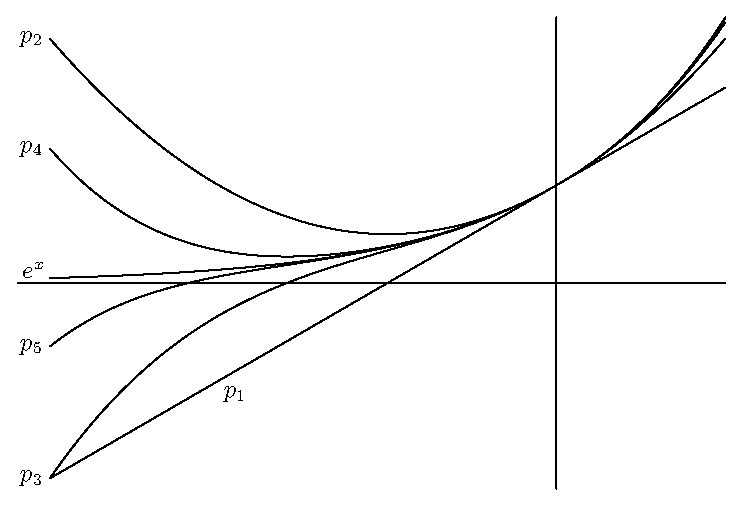
\includegraphics[width=12cm]{figure28.eps}
\caption{Polynomials Approximations to $e^x$.}
\label{figure-exponential-approximations}
\end{figure}

\begin{example}
Look at the exponential function $e^x$ centered at $\alpha =
0$. We have its Taylor series from the previous section. These
are its polynomial approximations. Their graphs are shown in
Figure \ref{figure-exponential-approximations}.

\begin{align*}
e^x & \cong \sum_{n=0}^1 \frac{1}{n!} x^n = 1 + x = p_1 \\
e^x & \cong \sum_{n=0}^2 \frac{1}{n!} x^n = 1 + x +
\frac{x^2}{2} = p_2 \\
e^x & \cong \sum_{n=0}^3 \frac{1}{n!} x^n = 1 + x +
\frac{x^2}{2} + \frac{x^3}{6} = p_3 \\
e^x & \cong \sum_{n=0}^4 \frac{1}{n!} x^n = 1 + x +
\frac{x^2}{2} + \frac{x^3}{6} + \frac{x^4}{24} = p_4 \\
e^x & \cong \sum_{n=0}^5 \frac{1}{n!} x^n = 1 + x +
\frac{x^2}{2} + \frac{x^3}{6} + \frac{x^4}{24} +
\frac{x^5}{120} = p_5
\end{align*}
\end{example}

\begin{figure}[t]
\centering
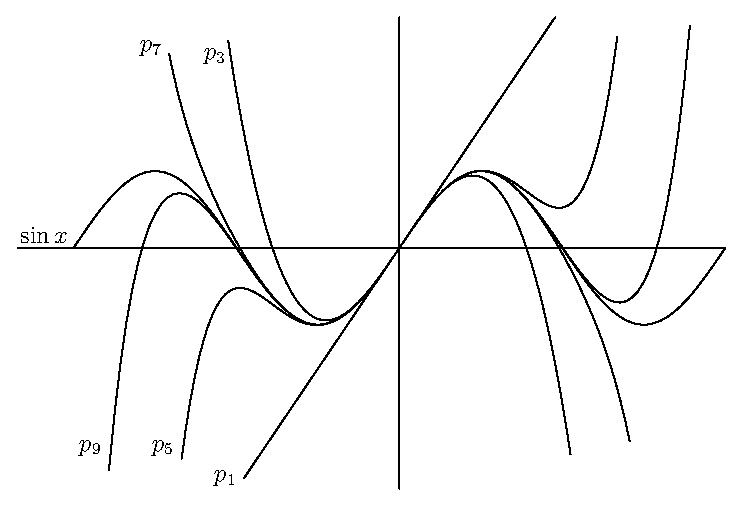
\includegraphics[width=12cm]{figure29.eps}
\caption{Polynomials Approximations to $\sin x$.}
\label{figure-sine-approximations}
\end{figure}

\begin{example}
The approximations for sine only have odd exponents, since there
are only odd monomials in the Taylor series for sine. These
are the first few approximations. Their graphs are shown in
Figure \ref{figure-sine-approximations}
\begin{align*}
\sin x & \cong \sum_{k=0}^0 \frac{(-1)^k}{(2k+1)!} x^{2k+1} =
x = p_1 \\
\sin x & \cong \sum_{k=0}^1 \frac{(-1)^k}{(2k+1)!} x^{2k+1} =
x - \frac{x^3}{3!} = p_3 \\
\sin x & \cong \sum_{k=0}^2 \frac{(-1)^k}{(2k+1)!} x^{2k+1} =
x - \frac{x^3}{3!} + \frac{x^5}{5!} = p_5 \\
\sin x & \cong \sum_{k=0}^3 \frac{(-1)^k}{(2k+1)!} x^{2k+1} =
x - \frac{x^3}{3!} + \frac{x^5}{5!} - \frac{x^7}{7!} = p_7 \\
\sin x & \cong \sum_{k=0}^4 \frac{(-1)^k}{(2k+1)!} x^{2k+1} =
x - \frac{x^3}{3!} + \frac{x^5}{5!} - \frac{x^7}{7!} +
\frac{x^9}{9!} = p_9 \\
\end{align*}
\end{example}

The main application of approximation is calculating values
of transcendental functions. We can't directly calculate their
values using basic arithmetic; we need a method. Before the
convenience of calculator and computer reference,
mathematicians, scientists and engineers carried around large
books of tables of values of trig, exponential and
logarithmic function. 

Polynomials are particularly useful as approximation tools
since they involve only the basic operations of arithmetic.
Computers can calculate with the basic operations of
arithmetic, so computers can understand polynomials. If we
want to program a computer or calculator to calculate values
of $e^x$ or $\sin x$ or $\ln x$ or some other transcendental
function, Taylor series are one of the best techniques. 

\begin{example}
The logarithm is a transcendental function which can't
be directly calculated. We had a Taylor series for the
logarithm in the previous section.
\begin{equation*}
-\ln (1-x) = \sum_{n=0}^\infty \frac{x^{n+1}}{n+1} dx
\end{equation*}
Using some clever arithmetic, we can write $\ln 2 = - \ln
\frac{1}{2} = - \ln \left( 1 - \frac{1}{2} \right)$. If we
truncate the series at degree $6$, we have this approximation
for $\ln 2$.
\begin{align*}
\ln 2 & \cong 1 \cdot \frac{1}{2} + \frac{1}{2} \cdot \left(
\frac{1}{2} \right)^2 + \frac{1}{3} \left( \frac{1}{2}
\right)^3 + \frac{1}{4} \left( \frac{1}{2} \right)^4 +
\frac{1}{5} \left( \frac{1}{2} \right)^5 + \frac{1}{6} \left(
\frac{1}{2} \right)^6 \\
\ln 2 & \cong \frac{1}{2} + \frac{1}{8} + \frac{1}{24} +
\frac{1}{64} + \frac{1}{160} + \frac{1}{384} \\
\ln 2 & \cong \frac{1327}{1920} = 0.6911458333333 \ldots 
= 0.6911458\bar{3}
\end{align*}
This is not to far off from the value of $\ln 2 =
0.69314\ldots$, accurate to the thousandths place. 
\end{example}

\begin{example}
There are many ways in mathematics to find approximations to
numbers. Recall that the alternating harmonic series also
summed to $\ln 2$. If we truncate that series after ten
steps, we get this approximation:
\begin{equation*}
\ln 2 \cong 1 - \frac{1}{2} + \frac{1}{3} - \frac{1}{4} +
\frac{1}{5} - \frac{1}{6} + \frac{1}{7} - \frac{1}{8} +
\frac{1}{9} - \frac{1}{10} = \frac{1627}{2520} =
0.645\overline{634920}
\end{equation*}
This expression is a poorer approximation for $\ln 2$; we
would need to go much farther down the alternating harmonic
series to match the precision of the Taylor series.
\end{example}

\end{document}
